\chapter{Calcul tensoriel}

    Dans ce chapitre, nous allons introduire toutes les notions de géométrie différentielle nécessaire pour la suite du cours. Nous avons vu que pour étudier un espace-temps courbe il faut introduire le concept de variété. La prochaine étape et de formaliser la notion de grandeur physique. Une grandeur physique est associée à un champ tensoriel sur la variété. Pour pouvoir mettre au point des équation qui décrivent ce grandeurs, on doit mettre au point une notion de dérivée pour les champ de tenseurs. On introduit alors trois opérateur différentiels : la dérivée extérieure (pour les $p$-forme), la dérivée de Lie (pour les champs de vecteurs) et finalement le dérivée covariante (pour les tenseurs). Le deux premiers opérateurs peuvent être défini à partir de la structure de variété mais le dernier nécessite une structure supplémentaire : la connexion. Ceci permettra décrire les équations du champ de matière qui régissent la gravité de manière covariante dans le chapitre suivant.
    
    \begin{rmk}
        Soit $Q_P$ un certain objets mathématique définit au point $P\in\M$, on peut alors lui associer le champ
        \begin{equation*}
            Q:P\in\M\mapsto Q_P
        \end{equation*}
        de sorte que toutes le propriété de $Q$ sont exactement les mêmes pour $Q_P$ si l'on se donne un point. Tout au long de ce chapitre, on se permettra de définir certaines quantités en un point $P$ en particulier et après d'utiliser ces notions sans spécifier le point; on fait en fait référence au champ associé. Ces notions de champs seront définies rigoureusement au cours du chapitre. Pour l'instant, c'est simplement une notation qui utilise le fait que les propriétés de $Q$ ne dépendent pas du point considéré.
    \end{rmk}
    
        \section{Vecteurs et tenseurs en géométrie différentielle}
        
            \subsection{Espace tangent}
                
                On peut se poser la question suivante : comment définir le déplacement en physique ? Imaginons être dans le vide, comment savoir si on se déplace ou pas ? S'il y a un champ dans cette région de l'espace (champ de densité de masse, champ électrique, ...), on peut dire que l'on est en mouvement si on observe une variation de ce champ. On pourrait aussi déduire que c'est le champ qui se déplace et que nous sommes fixe.  Si le champ est réparti dans tout l'espace, c'est une notion équivalente. Pour cela, on introduit la notion de vecteur tangent à un point d'une variété. Intuitivement, un vecteur tangent va être un objet permettant de mesurer la variation d'un champ $f:\M\to\mathbb{R}$ dans la direction du vecteur entre deux points très proches. Mathématiquement, on parle d'opérateur différentiel de premier ordre.
                
                \begin{definition}
                    Soit $\M$ une variété différentiable et $P\in\M$. Un \textit{vecteur tangent} à $\M$ en $P$ est une application linéaire $X_P:C^\infty(\M,\mathbb{R})\to\mathbb{R}$ telle que
                    \begin{equation}
                        X_P(fg) = X_P(f)g+fX_P(g)
                    \end{equation}
                    pour tout $f,g\in C^\infty(\M,\mathbb{R})$. Cette identité est appelée \textit{règle de Leibniz}.
                \end{definition}
                
                \begin{definition}
                    L'\textit{espace tangent} à $\M$ en $P$, noté $T_P\M$, est défini comme l'ensemble des vecteurs tangents à $\M$ en $P$.
                \end{definition}
                
                \begin{prop}
                \begin{leftbar}
                    L'espace tangent en un point est un espace vectoriel réel de même dimension que la variété.
                \end{leftbar}
                \end{prop}
                
                Cette définition abstraite ne donne pas beaucoup d'intuition sur la nature des vecteurs tangents. La règle de Leibniz fait penser aux dérivées, cependant définir une dérivée sur la variété n'est pas claire. Pour faire cela, on utilise le fait que les composantes $x^\mu$ des applications de coordonnées $x$ peuvent servir de "coordonnées" locales (tout en gardant à l'esprit que ces "coordonnées" sont des applications de $\M$ dans $\mathbb{R}$). On peut définir une dérivée en fonction des coordonnées locales comme
                \begin{equation}
                \frac{\p}{\p x^\mu}\bigg|_P:\left(
                \begin{array}{ccc}
                    C^\infty(\M,\mathbb{R}) & \longrightarrow & \mathbb{R} \\
                    f & \longmapsto & \frac{\p}{\p x^\mu}\bigg|_P(f) ~\hat{=}~ \frac{\p}{\p x^\mu}(f\circ x^{-1})(x^0(P),\dots,x^3(P))
                \end{array}
                \right).
                \end{equation}
                
                Il est claire que ces fonctions sont des vecteurs tangents en $P$ mais rien ne garanti que c'est la forme la plus générale. Il est en fait possible de montrer que n'importe quel vecteur tangent $X_P$ peut s'écrire comme une combinaison linéaire de dérivées partielles en fonction des coordonnées locales :
                \begin{equation}
                    X_P = \sum_{\mu=0}^3 X^\mu \frac{\p}{\p x^\mu}\bigg|_P
                \end{equation}
                où $V^\mu\in\mathbb{R}$.
                
                \begin{prop}\begin{leftbar}
                    L'ensemble
                    \begin{equation}
                        \left\{ \frac{\p}{\p x^\mu}\bigg|_P \right\}_{\mu=1,\dots,n}
                    \end{equation}
                    forme une base de $T_P\M$. Cette base est appellée \textit{base naturelle}.
                \end{leftbar}\end{prop}
                
                Cette définition abstraite de vecteur tangent rend le concept difficile à comprendre intuitivement. Si l'on se donne une ligne d'univers, on peut définir la notion de vecteur tangent à la ligne d'univers qui est plus intuitive.
                \begin{definition}
                    Soit une courbe différentiable $(\gamma)$ sur $\M$ de paramètre $t\in\mathbb{R}$. Si $f\in C^\infty(\M,\mathbb{R})$, on peut définir le \textit{vecteur tangent} à $\gamma$ en $\gamma(s)$ comme l'opérateur différentiel qui associe à $f$ sa dérivée le long de $\gamma$ évaluée en $\gamma(s)$:
                    \begin{equation}
                    \dot{\gamma}(s):\left(
                    \begin{array}{ccc}
                        C^\infty(\M,\mathbb{R}) & \longrightarrow & \mathbb{R} \\
                        f & \longmapsto &\dot{\gamma}(s)(f) ~\hat{=}~ \frac{d}{dt}f(\gamma(t))|_{t=s}
                    \end{array}
                    \right).
                    \end{equation}
                \end{definition}
                
                On vérifie facilement que $\dot{\gamma}(s)$ est bien un vecteur tangent. En effet, si $(U,\varphi)$ est une carte locale telle que $\gamma(s)\in U$, on peut écrire $\dot{\gamma}(s)$ on peut voir que
                \begin{equation}
                    \dot{\gamma}(s)(f) = \frac{d}{dt}f(\gamma(t))|_{t=s}= \frac{d(f\circ\varphi^{-1})(\varphi\circ\gamma(t))}{dt}|_{t=s}= \eval{\frac{d\gamma^\mu(t)}{dt}}_{t=s}\eval{\pdv{}{x^\mu}}_{\gamma(s)}(f)
                \end{equation}
                où $(\varphi\circ\gamma)(t)\equiv(\gamma^0(t),\dots,\gamma^{n-1}(t))$ et donc $\dot{\gamma}(s)$ s'écrit dans la base naturelle comme
                \begin{equation}
                     \dot{\gamma}(s) =  \eval{\frac{d\gamma^\mu(t)}{dt}}_{t=s}\eval{\pdv{}{x^\mu}}_{\gamma(s)}.
                \end{equation}
                Inversement, tout vecteur tangent en un point $P$ peut être vu comme un vecteur tangent à une courbe passant par $P$. Cette courbe n'est pas unique.\\
                
                Si l'on dispose de deux variétés $\M$ et $\N$ respectivement de dimension $m$ et $n$, et que 
                \begin{equation*}
                    \phi : M\to N
                \end{equation*}
                est une application différentiable, il y a une manière naturelle de définir une application entre les espaces tangents $T_P\M$ et $T_{\phi(P)}\N$. C'est la différentielle de l'application (ou "pushforward").
                
                \begin{definition}
                    Soit $\phi\in C^\infty(\M,\N)$, la \textit{différentielle de l'application} $\phi$ en $P\in\M$ est l'application linéaire
                    \begin{equation}
                        \phi_{*P}:\left(
                    \begin{array}{ccc}
                        T_P\M & \longrightarrow & T_{\phi(P)}\N \\
                        X & \longmapsto & \phi_*(X)
                    \end{array}
                    \right)
                    \end{equation}
                    définie par
                    \begin{equation}
                        \phi_{*P}(X)(f) = X(f\circ\phi)
                    \end{equation}
                    pour tout $X\in T_P\M$ et $f\in C^{\infty}(\N,\mathbb{R})$.
                \end{definition}
                
                La différentielle de l'application est une application linéaire entre deux espaces vectoriels de dimensions $m$ et $n$ respectivement. Elle associe à tout vecteur tangent à $\M$ en $P$ un vecteur tangent $\N$ en $\phi(P)$.
                
                \begin{rmk}
                    Pour alléger les notations, lorsque le contexte est clair nous n'indiquerons pas le point dont il est question pour la différentielle de l'application : $\phi_{*P}\equiv\phi_*$.
                \end{rmk}
                
                \begin{prop}\begin{leftbar}
                    Si $x^\mu$ sont des coordonnées locales en $P\in\M$ et $y^\mu$ sont des coordonnées locales en $\phi(P)\in\N$, la matrice associée à cette application linéaire est la jacobienne de $y\circ\phi\circ x^{-1}$ dans les bases $\eval{\pdv{}{x^\mu}}_{P}$ et  $\eval{\pdv{}{y^\mu}}_{\phi(P)}$. De sorte que, si $X = X^\mu\eval{\pdv{}{x^\mu}}_{P}\in T_P\M$, 
                    \begin{equation}
                        \phi_*(X) = X^\mu\eval{\pdv{(y\circ\phi\circ x^{-1})^\nu}{x^\mu(P)}(x^1(P),\dots,x^n(P))}_{x(P)}\eval{\pdv{}{y^\nu}}_{P}
                    \end{equation}
                \end{leftbar}\end{prop}
                
                Lorsque que l'on fait un changement de base dans l'espace tangent : 
                \begin{equation*}
                    \left\{\eval{\pdv{}{x^\mu}}_{P}\right\}\quad\to\quad \left\{\eval{\pdv{}{y^\mu}}_P\right\}
                \end{equation*}
                on a $\M=\N$ et $\phi = Id$. Dans ce cas, la matrice de changement de base est $\text{Jac}(y\circ x^{-1})$.\\
                
                Si $\phi$ est un difféomorphisme, on peut montrer que $\phi_*$ est isomorphisme linéaire. Des variétés qui sont difféomorphes ont donc des espaces tangent isomorphes. Réciproquement, si il existe un point $P\in\M$ tel que, en $P$, $\phi_*$ est un isomorphisme, alors il existe une voisinage $U$ autour de $P$ tel que $\phi$ restreint à ce voisinage soit un difféomorphisme de $U$ à $\phi(U)$.\\
                
                Un champ de vecteur $X$ sur une variété différentiable $\M$ est l'association d'un vecteur tangent de $T_P\M$ à chaque (ou un sous-ensemble) point $p\in\M$, cela peut être vu comme un champ de vitesses d'un ensemble de particule ou d'un fluide qui se déplace dans $\M$. Il est claire que, si l'on se donne un courbe différentiable sur $\M$, cette courbe définit un champ de vecteurs en associant à chaque point le long de la courbe le vecteur tangent à la courbe en ce point-là. Inversément, si l'on se donne un champ de vecteur sur $\M$ et un point $P\in\M$, il existe une seule courbe passant par ce point dont les vecteurs tangents sont donnés par ce champ de vecteurs. En revenant à l'analogie avec des particules : la particule qui passe par se point a une trajectoire unique définie par le champ de vecteur.
            
            \begin{definition}
             Soit $X$ un champ de vecteur sur $\M$. Une \textit{courbe intégrale} du champ $X$ est un couple $(I,\gamma)$ où est un ouvert de $\mathbb{R}$ contenant 0 et où $\gamma:I\to\M$ est une courbe différentiable telle que
             \begin{equation}
                 \dot{\gamma}(t) = X_{\gamma(t)}.
             \end{equation}
             Le point $P = \gamma(0)$ est la \textit{condition initiale} de $\gamma$.
            \end{definition}
            
            Dans des coordonnées locales $x^\mu$, si $X = X^\mu\p_\mu$ et que le courbe intégrale $\gamma$ a les coordonnées $x^\mu(t)$, on a la relation
            \begin{align}
                \dv{\gamma^\mu}{t} = X^\mu(x^1(t),\dots,x^n(t)).
            \end{align}
            
            Le théorème de Cauchy pour les fonctions lipschitziennes assure qu'une telle équation différentielle possède toujours une solution et qu'elle est unique pour une condition initiale donnée.
            
            \begin{prop}
            \begin{leftbar}
                Soit $X$ un champ de vecteurs sur $\M$. Pour tout $P\in\M$, il existe $\varepsilon>0$ et une unique courbe intégrale de $X$, $\gamma:(-\varepsilon,\varepsilon)\to\M$ de condition initiale $P$.
            \end{leftbar}
            \end{prop}
            
            \begin{definition}
            	Un \textit{invariant} pour le champ de vecteurs $X$ est une fonction le long des courbes intégrales de $X$. Si $x^\mu(t)$ sont les coordonnées d'une telle courbe passant par $x^\mu(0)$ et que $f\in C^\infty(\M,\mathbb{R})$ est un invariant alors
            	\begin{equation}
            		f(x^\mu(t)) = f(x^\mu(0))
            	\end{equation}
            	pour tout $t$.
            \end{definition}
            
            Par définition de courbe intégrale, cette condition est equivalente à 
            \begin{equation}
            V(f) = 0.
            \end{equation}
            
            \begin{exmp}
            	Soit $\M=\mathbb{R}^2$, les application de coordonnées $x,y$ et le champ de vecteurs
            	\begin{equation}
            		V = x\pdv{}{x}+\pdv{}{y}.
            	\end{equation}
            	Les courbes intégrales satisfont aux équations
            	\begin{align}
            		\dot{x}(t) &= x(t) \\
            		\dot{y}(t) &= 1
            	\end{align}
            	la fonction $f=xe^{-y}$ est un invariant de $V$.
            \end{exmp}
                
                
            
            \subsection{Espace cotangent}
            
                Comme tout espace vectoriel, l'espace tangent $T_P\M$ peut être vu comme le primal d'un espace dual $(T_P\M)^*$. Cet espace est composé des formes linéaires
                \begin{equation}
                    \omega:\left(
                \begin{array}{ccc}
                    T_P\M & \longrightarrow & \mathbb{R} \\
                    V & \longmapsto & \omega(V)
                \end{array}
                \right).
                \end{equation}
                Ces formes linéaires sont parfois appelées covecteurs.
                
                \begin{definition}
                    L'\textit{espace cotangent} à $\M$ en $P$ est le dual de l'espace tangent $\M$ en $P$, noté $(T_P\M)^*$.
                \end{definition}
                
                Pour rappel, si $\{e_\mu\}$ est une base de l'espace tangent $T_P\M$, on peut construire une unique base $\{e^\mu\}$ de $(T_P\M)^*$ associée à $\{e_\mu\}$ telle que
                \begin{equation}
                    e^\mu(e_\nu) = \delta^\mu_\nu.
                \end{equation}
                C'est la base duale. Dans ce cas, si $X\in T_P\M$ et $\omega\in (T_P\M)^*$ tels que $X = X^\mu e_\mu$ et $\omega = \omega_\mu e^\mu$, la forme linéaire $e^\mu$ envois $X$ sur $X^\mu$ :
                \begin{equation}
                    e^\mu(X) =  X^\nu e^\mu( e_\nu) = X^\nu \delta^\mu_\nu = X^\mu
                \end{equation}
                par linéarité. Inversement, on retrouve $\omega_\mu$ en appliquant $\omega$ sur $e_\mu$:
                \begin{equation}
                    \omega(e_\mu) = \omega_\nu e^\nu(e_\mu) = \omega_\nu \delta^\nu_\mu = \omega_\mu.
                \end{equation}
                
                \begin{definition}
                    A toute fonction $f\in C^\infty(\M,\mathbb{R})$ on peut faire correspondre un élément de l'espace dual $df_P\in(T_P\M)^*$ définit comme
                    \begin{equation}
                        df_P(X_P) = X_P[f]
                    \end{equation}
                    pour tout $X_P\in T_P\M$. Cette application est appelée la $\textit{différentielle}$ de $f$.
                \end{definition}
                Faire agir la différentielle d'une fonction sur un vecteur tangent revient à faire agir ce vecteur tangent sur la fonction.\\
                
                Pour l'espace tangent, nous avions vu que la donnée de coordonnées permet de définir une base naturelle. De la même manière, la donnée de coordonnées permet de définir une base naturelle de l'espace cotangent. Pour rappel, les coordonnée locales $x^\mu$ sont des applications de $\M$ dans $\mathbb{R}$ différentiables ce qui permet de considérer la différentielle de ses applications.
                
                \begin{prop}\begin{leftbar}
                    Si $x$ sont des coordonnées locales en $P\in\M$, alors l'ensemble $\{dx^\mu\}_{\mu=i,\dots,n}$ est la base duale de $\{\p_\mu\}_{\mu=i,\dots,n}$.
                \end{leftbar}\end{prop}
                
                \begin{proof}${}$\\
                    On retrouve la relation
                    \begin{equation}
                        dx^\nu(\p_\mu) = \p_\nu x^\mu = \delta^\mu_\nu.
                    \end{equation}
                    La base $\{dx^\mu\}_{\mu=i,\dots,n}$ est donc la base duale associée à la base $\{\p_\mu\}_{\mu=i,\dots,n}$ de l'espace tangent.
                \end{proof}
                
                \begin{rmk}
                    Maintenant que nous disposons des base naturelle pour $T_P\M$ et pour $(T_P\M)^*$, il faut garder à l'esprit que même si nous utilisons les notations abstraites $\{e_\mu\}$ et $\{e^\mu\}$, on peut toujours remplacer les $e_\mu$ par $\p_\mu$ et les $e^\mu$ par $dx^\mu$ par la donnée de coordonnées locales.
                \end{rmk}
                
                \begin{rmk}
                    Si $f\in C^\infty(\M,\mathbb{R})$ et $df\neq0$, la surface $f=\text{constante}$ de $\M$ est une variété de dimension $n-1$. Le sous-espace de $T_P\M$ qui contient tout les vecteurs $X$ tels que $df(X) = 0$ possède tout les vecteurs tangents à une courbe dans la surface $f=\text{constante}$ passant par $P$. On peut donc penser à $df$ comme la normale à la surface $f=\text{constante}$ en $P$.
                \end{rmk}
                
                \begin{prop}\begin{leftbar}
                    Soit $f:\in C^\infty(\M,\mathbb{R})$ une fonction quelconque et $x$ des coordonnées locales en $P\in\M$. L'application différentielle de $df$ peut se décomposer dans la base duale $dx^\mu$ associée aux coordonnées $x$ comme
                    \begin{equation}
                        df = \pdv{f}{x^\mu}dx^\mu.
                    \end{equation}
                \end{leftbar}\end{prop}
                
                \begin{proof}
                    Soit $X\in T_P\M$ tel que $X = X^\mu\pdv{}{x^\mu}$, alors par définition de $df$,
                    \begin{equation}
                        df(X) = X[f] = X^\mu\pdv{f}{x^\mu} = dx^\mu(X)\pdv{f}{x^\mu}
                    \end{equation}
                    quelque soit $X\in T_P\M$. Nous avons utilisé le fait que $dx^\mu(X) = X^\mu$. Pour finir, on retrouve bien
                    \begin{equation}
                        df = \pdv{f}{x^\mu}dx^\mu.
                    \end{equation}
                \end{proof}

                \begin{rmk}
                    Soit $\phi$ une fonction différentiable entre deux variétés $\M$ et $\N$. Si $\N=\mathbb{R}$, on retrouve les formes linéaires en remarquant que $T_P\mathbb{R}$ est assimilable à $\mathbb{R}$ lui-même. C'est pour cela que, si $f:\mathbb{R}^2\to\mathbb{R}$ est une fonction, on dit que $df$ est la différentielle de $f$ et que
                    \begin{equation}
                        df = \frac{\p f}{\p x} dx + \frac{\p f}{\p y} dy.
                    \end{equation}
                    Ce n'est rien d'autre que la décomposition du vecteur $df\in T_{(x,y)}\mathbb{R}^2$ dans la base duale $\{dx,dy\}$.
                \end{rmk}
                
                Étant donné que $\{dx^\mu\}$ forme une base de $(T_P\M)^*$, quelque soit $\omega\in(T_P\M)^*$, on peut écrire
                \begin{equation}
                    \omega = \omega_\mu~dx^\mu
                \end{equation}
                avec $\omega_\mu\in\mathbb{R}$. Notons que les $\p_\mu$ sont bien covariants, les $V^\mu$ contravariants, les $dx^\mu$ contravariants et les $w_\mu$ covariants. Ceci est vrai quel que soit l'espace vectoriel en question. On éclaircira ça dans la section suivante. Il est aussi important de remarquer que lorsque l'on considère des changements de base dans cette partie, on parle de changement de base quelconque, et pas forcément des transformations de Lorentz.\\
                
                Si $\phi:\M\to\N$ est différentiable, on peut définir la différentielle de l'application $\phi$ entre les espaces tangents de $\N$ et $\M$, notée $\phi_*$, comme vu dans la section précédente. Maintenant que nous étudions les espaces tangents duaux, on peut définir, à partir de $\phi_*$, une application qui associe à chaque forme linéaire de $(T_{\phi(P)}\N)^*$ une forme linéaire de $(T_P\M)^*$. C'est la transposée de l'application (ou "pullback").
                
                \begin{definition}
                    Soit $\phi\in C^\infty(\M,\N)$, la \textit{transposée de l'application} $\phi$ en $P\in\M$ est l'application linéaire
                    \begin{equation}
                        \phi^{*P}:\left(
                    \begin{array}{ccc}
                        (T_{\phi(P)}\N)^* & \longrightarrow & (T_P\M)^* \\
                        \omega & \longmapsto & \phi^{*P}(\omega)
                    \end{array}
                    \right)
                    \end{equation}
                    définie par
                    \begin{equation}
                        \phi^{*P}(\omega)(X) = \omega(\phi_{*P}(X))
                    \end{equation}
                    pour tout $\omega\in (T_{\phi(P)}\N)^*$ et $X\in T_P\M$.
                \end{definition}
            
            \subsection{Tenseurs}
                
                Définissons au préalable l'espace vectoriel
                \begin{equation}
                    \Pi^q_p ~\hat{=}~ \underbrace{(T_P\M)^*\times\dots\times (T_P\M)^*}_{\text{$p$ facteurs}}\times\underbrace{T_P\M\times\dots\times T_P\M}_{\text{$q$ facteurs}}.
                \end{equation}
                
                \begin{definition}
                    Un $\tens{p}{q}$-\textit{tenseur} (ou \textit{tenseur} de type $(p,q)$) en $P$ est une application linéaire en chaque argument
                    \begin{equation}
                        T:\left(
                    \begin{array}{ccc}
                        \Pi^q_p & \longrightarrow & \mathbb{R} \\
                        (\omega^1,\dots,\omega^p,X_1,\dots,X_q) & \longmapsto & T(\omega^1,\dots,\omega^p,X_1,\dots,X_q)
                    \end{array}
                    \right).
                    \end{equation}
                \end{definition}
                
                Par définition,
                \begin{itemize}[label = \textbullet]
                    \item les tenseur de type $(0,0)$ sont les scalaires de $\mathbb{R}$
                    \item les tenseur de type $(0,1)$ sont les covecteurs, c'est-à-dire les éléments de $(T_P\M)^*$
                    \item les tenseur de type $(1,0)$ sont les éléments de $(T_P\M)^{**}$, mais comme $(T_P\M)^{**}\cong T_P\M$, on identifie les vecteur $X$ au tenseur $(1,0)$ dont l'action sur $\omega\in(T_P\M)^*$ est définie par
                    \begin{equation}
                        X(\omega)~\hat{=}~\omega(X).
                    \end{equation}
                \end{itemize}
                
                \begin{definition}
                    L'\textit{espace des tenseurs} de type $(p,q)$ en $P$ est noté
                    \begin{equation}
                        T^{(p,q)}_P\M = \underbrace{T_P\M\otimes\dots\otimes T_P\M}_{\text{$p$ facteurs}}\otimes \underbrace{(T_P\M)^*\otimes\dots\otimes (T_P\M)^*}_{\text{$q$ facteurs}}.
                    \end{equation}
                \end{definition}
                
                On écrit $X_1\otimes\dots\otimes X_p\otimes\omega^1\otimes\omega^q$ le tenseur qui envois $(\eta^1,\dots,\eta^p,Y_1,\dots,Y_p)$ sur
                \begin{equation}
                    \eta^1(X_1)\dots\eta^p(X_p)\omega^1(Y_1)\dots\omega^q(Y_q).
                \end{equation}
                
                \begin{leftbar}
                \begin{prop}
                    On a $dim(T_P^{(0,p)}(\M)) = n^p$.
                \end{prop}
                \end{leftbar}
                
                \begin{proof}
                    Calculer le nombre de tenseurs linéairement indépendants revient à calculer le nombre de manière de faire le produit tensoriel de $p$ vecteurs avec à chaque fois $n$ choix par vecteurs. On trouve bien $n^p$.
                \end{proof}
                
                \begin{definition}
                    Soit $\{e_\mu\}$ une base de $T_P\M$ et $\{e^\mu\}$ la base duale de $(T_P\M)^*$. Si $T$ est un tenseur de type $(p,q)$, on appelle \textit{composantes du tenseur} $T$ les nombres
                    \begin{equation}
                        T\indices{^{\mu_1\dots\mu_p}_{\nu_1\dots\nu_q}}~\hat{=}~T(e^{\mu_1},\dots,e^{\mu_p},e_{\nu_1},\dots,e_{\nu_q})\in\mathbb{R}.
                    \end{equation}
                \end{definition}
                
                \begin{prop}\begin{leftbar}
                    Si $T$ est un tenseur de type $(p,q)$, alors
                    \begin{equation}
                        T(\omega^1,\dots,\omega^p,X_1,\dots,X_q) = \omega^1_{\mu_1}\dots\omega^p_{\mu_p}X^{\nu_1}_1\dots X^{\nu_q}_q~ T\indices{^{\mu_1\dots\mu_p}_{\nu_1\dots\nu_q}}.
                    \end{equation}
                \end{leftbar}\end{prop}
                
                \begin{proof}
                    Soient $\omega^1,\dots,\omega^p\in(T_P\M)^*$ et $X_1,\dots,X_q\in T_P\M$ tels que 
                    \begin{align}
                        \omega^i &= \omega^i_\mu ~dx^\mu \\
                        X_j &= X^\mu_j~\p_\mu
                    \end{align}
                    pour $i=1,\dots,p$ et $j=1,\dots,q$. Dans ce cas, comme $T$ est linéaire selon chaque argument,
                    \begin{align}
                        T(\omega^1,\dots,\omega^p,X_1,\dots,X_q) &= T(\omega^1_{\mu_1}e^{\mu_1},\dots,\omega^p_{\mu_p}e^{\mu_p},X^{\nu_1}_1e_{\nu_1},\dots,X^{\nu_q}_qe_{\nu_q}) \\
                        &=\omega^1_{\mu_1}\dots\omega^p_{\mu_p}X^{\nu_1}_1\dots X^{\nu_q}_q~T(e^{\mu_1},\dots,e^{\mu_p},e_{\nu_1},\dots,e_{\nu_q}) \\
                        &= \omega^1_{\mu_1}\dots\omega^p_{\mu_p}X^{\nu_1}_1\dots X^{\nu_q}_q~ T\indices{^{\mu_1\dots\mu_p}_{\nu_1\dots\nu_q}}
                    \end{align}
                \end{proof}
                
                \begin{exmp}${}$
                    \begin{itemize}[label = \textbullet]
                        \item le tenseur métrique $g_{\mu\nu}$ est un tenseur de type $(0,2)$
                        \item le tenseur métrique $g^{\mu\nu}$ est un tenseur de type $(2,0)$
                        \item la quadri-vitesse $U^{\mu}$ le long d'une ligne d'univers est un tenseur de type $(1,0)$. Cependant, la quadri-accélération n'est pas un tenseur.
                        \item le tenseur électromagnétique $F_{\mu\nu}$ est un tenseur de type $(0,2)$
                        \item le quadri-potentiel $A_{\mu}$ est un tenseur de type $(0,1)$
                    \end{itemize}
                \end{exmp}
                
                \begin{leftbar}
                \begin{prop}
                    Le delta de Kronecker définit un tenseur qui ont la particularité d'avoir les mêmes composantes dans n'importe quelle base.
                \end{prop}
                \end{leftbar}
                
                La propriété fondamentale des tenseurs est la loi de transformation de leurs composantes.
                
                \begin{prop}\begin{leftbar}
                    Soit $T$ un tenseur de type $(p,q)$ de composantes $T\indices{^{\mu_1\dots\mu_p}_{\nu_1\dots\nu_q}}$ dans les coordonnées $x$. Les composantes de $T$ dans les coordonnées $x'$ s'expriment comme 
                    \begin{equation}
                        {T'}\indices{^{\mu_1\dots\mu_p}_{\nu_1\dots\nu_q}} = \pdv{x'^{\mu_1}}{x^{\sigma_1}} (P)\dots\pdv{x'^{\sigma_p}}{x^{\sigma_p}}(P)\pdv{x^{\rho_1}}{x'^{\nu_1}}(P)\dots\pdv{x^{\rho_q}}{x'^{\nu_q}}(P)~T\indices{^{\sigma_1\dots\sigma_p}_{\rho_1\dots\rho_q}}
                    \end{equation}
                \end{leftbar}\end{prop}
                
                \begin{proof}${}$\\
                    Si $V\in T_P\M$ et $V^\mu\p_\mu$ dans les coordonnées locales $x^\mu$. Dans d'autres coordonnées locales $x'^\mu$, on a la matrice de changement de base (jacobienne) $ \frac{\p x'^\mu}{\p x^\nu}$ et $\omega = \omega_\mu~dx^\mu$, alors
                    \begin{equation}
                        V[\phi] = V^\mu \frac{\p\phi}{\p x^\mu} =  \underbrace{V^\mu\frac{\p x'^\nu}{\p x^\mu}}_{V'^\nu}\frac{\p\phi}{\p x'^\nu}
                    \end{equation}
                    pour tout $\phi\in C^\infty(\M,\mathbb{R})$, avec $V'^\mu = V^\nu\frac{\p x'^\mu}{\p x^\nu}$. Et donc les $V^\mu$ sont des tenseurs de type $(1,0)$ car ils se transforment de la manière souhaitée. Si $\omega\in (T_P\M)^*$ et $w_\mu dx^\mu$ dans les coordonnées locales $x^\mu$. Pour d'autres coordonnées locales $x'^\mu$ on a la matrice de changement de base (jacobienne) $ \frac{\p x^\mu}{\p x'^\nu}$ et $\omega = \omega_\mu~dx^\mu$, alors
                    \begin{equation}
                        \omega = T_P^{(0,1)\M} = \omega_\mu~dx^\mu =  \underbrace{\omega_\mu \frac{\p x^\mu}{\p x'^\nu}}_{w'_\nu}dx'^\nu
                    \end{equation}
                    donc les $\omega_\mu$ sont bien des tenseurs de type $(0,1)$. Le cas générale est direct en utilisant la linéarité du produit tensoriel.
                \end{proof}
                
                \begin{definition}
                    Un tenseur de type $(1,0)$ est appelé \textit{vecteur} et un tenseur de type $(0,1)$ est appelé \textit{1-forme}.
                \end{definition}
                
                \begin{prop}\begin{leftbar}
                    L'espace tangent est un espace de vecteurs, c'est-à-dire que les vecteur tangent se transforment bien comme des vecteurs.
                    \begin{equation}
                        T_P\M = T^{(1,0)}_P\M
                    \end{equation}
                \end{leftbar}\end{prop}
                
                La loi de transformation est bien celle d'un vecteur. Ceci justifie le nom de "vecteur" tangent.\\
                
                \begin{prop}\begin{leftbar}
                    L'espace dual de l'espace tangent est l'espace des 1-formes.
                    \begin{equation}
                        (T_P\M)^* \equiv \Omega_1(\M)
                    \end{equation}
                \end{leftbar}\end{prop}
                
                Discutons des opérations que l'on peut faire entre tenseurs.
                
                \begin{prop}[opérations sur les tenseurs]\begin{leftbar}
                    Nous pouvons effectuer les opérations suivantes entre tenseurs :
                    \begin{enumerate}[label = \textit{\roman*)}]
                        \item combinaison linéaire : si $t_1$ et $t_2$ sont de type $(p,q)$,
                        \begin{equation}
                            \alpha t_1 + \beta t_2, \qquad\alpha,\beta\in\mathbb{R}
                        \end{equation} 
                        est un tenseur de type $(p,q)$.
                        \item produit tensoriel : si $t_1$ est de type $(p_1,q_1)$ et $t_2$ ets de type $(p_2,q_2)$ alors
                        \begin{equation}
                            (t_1\otimes t_2)_{\qquad\qquad b_1\dots b_{q_1+q_2}}^{a_1\dots a_{p_1+p_2}} =
                            t_1^{a_1\dots a_{p_1}}{}_{b_1\dots b_{q_1}}~t_2^{a_{p_1+1}\dots a_{p_1+p_2}}{}_{b_{q_1+1}\dots b_{q_1+q_2}}
                        \end{equation}
                        est un tenseur de type $(p_1+p_2,q_1+q_2)$.
                        \item contraction : si $t$ est un tenseur de type $(p,q)$ alors
                        \begin{equation}
                            T^{a_1\dots a_{i-1}a_{i+1}\dots a_p}{}_{b_1\dots b_{j-1}b_{j+1}\dots b_q} = t^{a_1\dots a_{i-1} a a_{i+1}\dots a_p}{}_{b_1\dots b_{j-1} a b_{j+1}\dots b_q}
                        \end{equation}
                        est un tenseur de type $(p-1,q-1)$.
                    \end{enumerate}
                \end{leftbar}\end{prop}
                
                \begin{proof}
                    Les trois propriétés se démontrent en observant comment les objets définis ci-dessus se transforment lors d'un changement de coordonnées.
                \end{proof}
                
                \begin{rmk}
                    On peut définir plus rigoureusement la contraction du $i$-ème ($1\leq i\leq p$) et du $j$-ème ($1\leq j\leq q$) indice d'un tenseur de type $(p,q)$ comme l'image de l'application contraction $C^i_j$ définie comme
                    \begin{equation}
                        C^i_j:\left(
                    \begin{array}{ccc}
                        T^{(p,q)}_P\M & \longrightarrow & T^{(p-1,q-1)}_P\M \\
                        T & \longmapsto & C^i_j(T)
                    \end{array}
                    \right)
                    \end{equation}
                    avec 
                    \begin{equation}
                        C^i_j(T) = T\indices{^{\mu_1\dots\mu_{i-1}a\mu_{i+1}\dots\mu_p}_{\nu_1\nu_{j-1}a\nu_{j+1}\dots\nu_q}} e_{\mu_1}\otimes\dots\otimes e_{i-1}\otimes  e_{i+1}\otimes\dots\otimes e_{\mu_p}\otimes e^{\nu_1}\otimes\dots\otimes e^{j-1}\otimes e^{j+1}\otimes\dots\otimes e^{\nu_q}.
                    \end{equation}
                    Le tenseur $C^i_j(T)$ est indépendant de la base choisie. On peut également contracter des indices covariants entre-eux ou des indices contravariants entre-eux cependant le résultat n'est plus indépendant du choix de base.
                \end{rmk}
                
                \begin{exmp}${}$
                    \begin{itemize}[label = \textbullet]
                        \item Soit $F_{\mu\nu}$ un tenseur de type $(0,2)$ et $g^{\mu\nu}$ un tenseur de type $(2,0)$. Alors $T\indices{^\sigma^\rho_\mu_\nu}~\hat{=}~F_{\mu\nu}g^{\sigma\rho}$ est un tenseur de type $(2,2)$.
                        \item Soit $t\indices{^a^b_c}$ un tenseur de type $(2,1)$. Il y a deux contractions distinctes : $T_1^a~\hat{=}~t\indices{^b^a_b}$ et $T_2^a~\hat{=}~t\indices{^a^b_b}$. Ce sont tout deux des tenseurs de type $(1,0)$.
                        \item Soit $F_{\mu\nu}$ un tenseur de type $(0,2)$ et $H^{\mu\nu\rho}$ un tenseur de type $(3,0)$. Alors $T\indices{^\mu^\nu_\sigma}~\hat{=}~H^{\mu\nu\rho}F_{\rho\sigma}$ est un tenseur de type $(2,1)$. On a utilisé le produit tensoriel et la contraction.
                    \end{itemize}
                \end{exmp}
                
                Avec le produit $\otimes$, l'espace des tenseurs en $P$ forme une algèbre sur $\mathbb{R}$.
                
                \begin{prop}\begin{leftbar}
                    Soit $T$ est un tenseur de type $(p,q)$ de composantes $T\indices{^{\mu_1\dots\mu_p}_{\nu_1\dots\nu_q}}$, alors
                    \begin{equation}
                        T = T\indices{^{\mu_1\dots\mu_p}_{\nu_1\dots\nu_q}} e_{\mu_1}\otimes\dots\otimes e_{\mu_p}\otimes e^{\nu_1}\otimes\dots\otimes e^{\nu_q}
                    \end{equation}
                \end{leftbar}\end{prop}
                
                \begin{proof}
                    D'une part, nous avons la relation
                    \begin{equation}
                         T(\omega^1,\dots,\omega^p,X_1,\dots,X_q) = \omega^1_{\mu_1}\dots\omega^p_{\mu_p}X^{\nu_1}_1\dots X^{\nu_q}_q~ T\indices{^{\mu_1\dots\mu_p}_{\nu_1\dots\nu_q}}.
                    \end{equation}
                    D'autre part, comme $T$ est un tenseur, il est toujours possible de l'exprimer comme une combinaison linéaire de vecteurs de la base de $T^{(p,q)}_P\M$. Notons $\widetilde{T}\indices{^{\mu_1\dots\mu_p}_{\nu_1\dots\nu_q}}$ les coefficients de cette décomposition.
                    \begin{equation}
                        T = \widetilde{T}\indices{^{\mu_1\dots\mu_p}_{\nu_1\dots\nu_q}} e_{\mu_1}\otimes\dots\otimes e_{\mu_p}\otimes e^{\nu_1}\otimes\dots\otimes e^{\nu_q}
                    \end{equation}
                    Dans ce cas, par propriété de base duale,
                    \begin{align}
                        T(\omega^1,\dots,\omega^p,X_1,\dots,X_q) &= \widetilde{T}\indices{^{\mu_1\dots\mu_p}_{\nu_1\dots\nu_q}} (e_{\mu_1}\otimes\dots\otimes e_{\mu_p}\otimes e^{\nu_1}\otimes\dots\otimes e^{\nu_q})(\omega^1,\dots,\omega^p,X_1,\dots,X_q)\\
                        &= \omega^1_{\alpha_1}\dots\omega^p_{\alpha_p}X^{\beta_1}_1\dots X^{\beta_q}_q \widetilde{T}\indices{^{\mu_1\dots\mu_p}_{\nu_1\dots\nu_q}} \delta^{\alpha_1}_{\mu_1}\dots\delta^{\alpha_p}_{\mu_p}\delta^{\nu_1}_{\beta_1}\dots\delta^{\nu_q}_{\beta_q}\\
                        &= \omega^1_{\mu_1}\dots\omega^p_{\mu_p}X^{\nu_1}_1\dots X^{\nu_q}_q~ \widetilde{T}\indices{^{\mu_1\dots\mu_p}_{\nu_1\dots\nu_q}}
                    \end{align}
                    Donc, 
                    \begin{equation}
                        \widetilde{T}\indices{^{\mu_1\dots\mu_p}_{\nu_1\dots\nu_q}} = T\indices{^{\mu_1\dots\mu_p}_{\nu_1\dots\nu_q}}.
                    \end{equation}
                    car ca doit être vrai pour tout $\omega^1,\dots,\omega^p,X_1,\dots,X_q$.
                \end{proof}
                
                \begin{rmk}
                    La proposition qui précède montre que, si l'on se donne une base de $T_P\M$ et une base de $(T_P\M)^*$, il y a une correspondance biunivoque entre l'ensemble des composantes d'un tenseur et le tenseur lui-même. Et pour rappel, se donner des coordonnées locales $x$ induit une base naturelle de $T_P\M$ et de $(T_P\M)^*$. Si l'on dispose de coordonnées locales, nous ferons donc souvent l'abus de langage de dire que les composantes d'un tenseur sont un tenseur pour en fait désigner le tenseur que ses composantes définissent.
                \end{rmk}
                
                Les composantes de tenseurs possèdent des propriétés de symétrie par rapport à une partie de leurs indices. Les définitions suivantes énoncent différentes propriétés possibles. Ces définitions sont utiles uniquement si elles sont accompagnées de propositions qui disent que de tels tenseurs existent et que ces propriétés sont indépendantes de la base choisie. Nous supposerons que c'est le cas.
                
                \begin{definition}
                    On appelle \textit{tenseur covariant complètement symétrique} un tenseur $t$ satisfaisant à
                    \begin{equation}
                            t_{a_1\dots a_p} = t_{a_{\sigma(1)}\dots a_{\sigma(p)}}
                    \end{equation}
                    pour tout $\sigma\in S_p$. Lorsque tous les indices sont contravariants, c'est un \textit{tenseur contravariant complètement symétrique}.
                \end{definition}
                
                \begin{definition}
                    On appelle \textit{tenseur covariant complètement anti-symétrique} un tenseur $t$ satisfaisant à
                    \begin{equation}
                            t_{a_1\dots a_p} = \varepsilon(\sigma)t_{a_{\sigma(1)}\dots a_{\sigma(p)}}
                    \end{equation}
                    pour tout $\sigma\in S_p$. Lorsque tous les indices sont contravariants, c'est un \textit{tenseur contravariant complètement anti-symétrique}.
                \end{definition}
                
                Il est aussi possible que des tenseurs soient symétriques (ou anti-symétriques) seulement sous permutation d'une certaine partie de leurs indices. Ou encore, comme on l'a vu avec l'identité de Bianchi, que des tenseurs satisfassent une condition mettant en jeu une certaine combinaison linéaire de composantes.\\
                
                \begin{definition}
                    Soit $t$ un tenseur de type d'ordre $p$. On introduit les notations suivantes: la \textit{partie symétrique} de $t$ est 
                    \begin{equation}
                        t_{(a_1\dots a_p)} ~\hat{=}~ \frac{1}{p!} \sum_{\sigma\in S_p}t_{a_{\sigma(1)}\dots a_{\sigma(p)}}.
                    \end{equation}
                    La \textit{partie anti-symétrique} de $t$ est 
                    \begin{equation}
                        t_{[a_1\dots a_p]} ~\hat{=}~ \frac{1}{p!} \sum_{\sigma\in S_p}\varepsilon(\sigma) t_{a_{\sigma(1)}\dots a_{\sigma(p)}}.
                    \end{equation}
                 \end{definition}
                
                \begin{prop}\begin{leftbar}
                    Soit $t$ un tenseur d'ordre $p$.
                    \begin{enumerate}[label = \textit{\roman*)}]
                        \item la partie symétrique de $t$ est anti-symétrique i.e. on peut toujours symétriser ce tenseur comme
                        \begin{equation}
                            t_{(a_1\dots a_p)} = \frac{1}{p!} \sum_{\sigma\in S_p} t_{a_{\sigma(1)}\dots a_{\sigma(p)}}.
                        \end{equation}
                        \item la partie anti-symétrique de $t$ est anti-symétrique i.e. on peut toujours anti-symétriser ce tenseur comme
                        \begin{equation}
                            t_{[a_1\dots a_p]} = \frac{1}{p!} \sum_{\sigma\in S_p}\varepsilon(\sigma) t_{a_{\sigma(1)}\dots a_{\sigma(p)}}.
                        \end{equation}
                    \end{enumerate}
                \end{leftbar}\end{prop}
                
                \begin{proof}${}$
                    \begin{enumerate}[label = \textit{\roman*)}]
                        \item On voit clairement que l'expression est complètement symétrique.
                        \item De même que que précédemment, on voit clairement que l'expression est complètement anti-symétrique.
                    \end{enumerate}
                \end{proof}
                
                \begin{prop}\begin{leftbar}
                    Soit $t$ un tenseur d'ordre $p$.
                    \begin{enumerate}[label = \textit{\roman*)}]
                        \item $t$ est complètement symétrique si et seulement si
                        \begin{equation}
                            t_{(a_1\dots a_p)} = t_{a_1\dots a_p}
                        \end{equation}
                        \item $t$ est complètement anti-symétrique si et seulement si
                        \begin{equation}
                            t_{[a_1\dots a_p]} = t_{a_1\dots a_p}
                        \end{equation}
                    \end{enumerate}
                \end{leftbar}\end{prop}
                
                \begin{proof}${}$
                    \begin{enumerate}[label = \textit{\roman*)}]
                        \item Nous faisons uniquement le cas anti-symétrique. Le cas symétrique est le même mais sans les $\varepsilon(\sigma)$.
                        \item Si $t$ est complètement anti-symétrique, alors 
                        \begin{equation}
                            t_{a_1\dots a_p} = \varepsilon(\sigma)t_{a_{\sigma(1)}\dots a_{\sigma(p)}}
                        \end{equation}
                        et donc
                        \begin{align}
                            t_{[a_1\dots a_p]} &= \frac{1}{p!}\sum_{\sigma\in S_p}\varepsilon(\sigma) t_{a_{\sigma(1)}\dots a_{\sigma(p)}}\\
                            &= \frac{1}{p!}\sum_{\sigma\in S_p}\varepsilon(\sigma)^2 t_{a_1\dots a_p}\\
                            &= t_{a_1\dots a_p} \frac{1}{p!}\sum_{\sigma\in S_p}1\\
                            &= t_{a_1\dots a_p}
                        \end{align}
                        Inversement, si
                        \begin{equation}
                            t_{a_1\dots a_p} = t_{[a_1\dots a_p]}
                            = \frac{1}{p!}\sum_{\sigma\in S_p}\varepsilon(\sigma) t_{a_{\sigma(1)}\dots a_{\sigma(p)}}
                        \end{equation}
                        alors, pour une certaine permutation $\sigma'\in S_p$,
                        \begin{align}
                            t_{a_{\sigma'(1)}\dots a_{\sigma'(p)}} &=  \frac{1}{p!}\sum_{\sigma\in S_p}\varepsilon(\sigma) t_{a_{(\sigma\circ\sigma')(1)}\dots a_{(\sigma\circ\sigma')(p)}}\\
                            &= \frac{1}{p!}\bigg( \varepsilon(\sigma'^{-1}) t_{a_{(\sigma'^{-1}\circ\sigma')(1)}\dots a_{(\sigma'^{-1}\circ\sigma')(p)}}+\sum_{\substack{\sigma\in S_p\\\sigma\neq\sigma'^{-1}}} \varepsilon(\sigma) t_{a_{(\sigma\circ\sigma')(1)}\dots a_{(\sigma\circ\sigma')(p)}} \bigg)\\
                            &= \frac{1}{p!}  \varepsilon(\sigma')t_{a_1\dots a_p}
                        \end{align}
                        La dernière égalité vient du fait que $ \varepsilon(\sigma'^{-1}) =  \varepsilon(\sigma')$ et que le terme avec la somme s'annule. En effet,
                        \begin{align}
                            \sum_{\substack{\sigma\in S_p\\\sigma\neq\sigma'^{-1}}} \varepsilon(\sigma) t_{a_{(\sigma\circ\sigma')(1)}\dots a_{(\sigma\circ\sigma')(p)}} 
                            &= \sum_{\substack{\sigma\in S_p\\\sigma\neq id}} \varepsilon(\sigma\circ\sigma') t_{a_{\sigma(1)}\dots a_{\sigma(p)}} \\
                            &= \varepsilon(\sigma')\sum_{\substack{\sigma\in S_p\\\sigma\neq id}} \varepsilon(\sigma) t_{a_{\sigma(1)}\dots a_{\sigma(p)}}\\
                            &= \varepsilon(\sigma') p!\underbrace{\left( t_{[a_1\dots a_p]}-t_{a_1\dots a_p} \right)}_{0}
                        \end{align}
                    \end{enumerate}
                \end{proof}
                
                \begin{exmp}
                    Pour un tenseur d'ordre $2$,
                    \begin{equation}
                        t_{[ab]} = \frac{1}{2}(t_{ab}-t_{ba})
                    \end{equation}
                    ce qui est clairement anti-symétrique sous l'échange de $a$ et $b$. 
                \end{exmp}
                
                \begin{prop}\begin{leftbar}
                    Tout tenseur $t$ d'ordre $p$ peut être décomposé comme
                    \begin{equation}
                        t_{a_1\dots a_p} = t_{(a_1\dots a_p)} + t_{[a_1\dots a_p]}
                    \end{equation}
                \end{leftbar}\end{prop}
                
                \begin{proof}${}$\\
                    \comp
                \end{proof}
                
                \begin{rmk}
                    On peut voir que le principe de projection émerge. Un tenseur non-nul ne peut pas être symétrique et anti-symétrique à la fois et tout tenseur peut se décomposer comme la somme de sa partie symétrique et sa parti symétrique.
                \end{rmk}
                
                Comme il a déjà été mentionné, la donnée d'un système de coordonnées rend les notion de tenseur et de coordonnée de tenseur équivalentes. Pour les tenseurs d'ordre $2$, on peut associer une matrice dont les éléments sont les composantes du tenseur.\\
                
                \begin{definition}
                    Soit un tenseur $t$ d'ordre $2$. On dit que ce tenseur est \textit{non-dégénéré} si la matrice de ses composantes est inversible.
                \end{definition}
                
                Remarquons que la notion de dégénérescence dépend du point $P$ considéré.
                
            \subsection{Tenseur métrique}
                
                \begin{definition}
                    Un \textit{tenseur métrique} est un tenseur de type $(0,2)$ non-dégénéré et complètement symétrique.
                \end{definition}
                
                \begin{prop}\begin{leftbar}
                    Le tenseur métrique définit, en chaque point $P\in\M$, un pseudo-produit scalaire sur $T_P\M$.
                \end{leftbar}\end{prop}
                
                \begin{proof}
                    Soit $g$ un tenseur métrique, étant donné qu'il est deux fois covariant, $g$ définit en chaque point $P\in\M$, une forme bilinéaire symétrique non-dégénérée.
                \begin{equation}
                    g:\left(
                \begin{array}{ccc}
                    T_P\M\times T_P\M & \longrightarrow & \mathbb{R} \\
                    (V,W) & \longmapsto & g_{ab}V^a W^b
                \end{array}
                \right).
                \end{equation}
                où $V^a$ et $W^b$ sont les composantes de $V$ et $W$ dans une base choisie de $T_P\M$. De plus, pour tout $V,W\in T_P\M$,
                \begin{equation}
                    g(V,W) = g(W,V)
                \end{equation}
                ce qui définit bien un pseudo-produit scalaire.
                \end{proof}
                
                Un tel tenseur est caractérisé par sa signature $(r,s)$, où $r+s = \text{dim}(\M) = n$. Dans le cas euclidien, nous avons $(r,s) = (0,n)$. Dans le cas lorentzien, $(r,s) = (1,n-1)$.
                
                \begin{prop}\begin{leftbar}
                    Le tenseur inverse $g^{ab}$ (tenseur dont les composantes sont celle de la matrice inverse de $g_{ab}$) définit, en chaque point $P\in\M$, un produit scalaire sur $(T_P\M)^*$.
                \end{leftbar}\end{prop}
                
                \begin{proof}
                    Considérons une matrice de changement de base $M$ (par forcément une transformation de Lorentz). On a
                    \begin{align}
                        g'_{ab} &= g_{ab}M_{a}^{~c}M_{b}^{~d}\\
                        \Leftrightarrow \quad g'&= MgM^T \\
                        \Leftrightarrow \quad g &= (M^T)^{-1}g^{-1}M^{-1}
                    \end{align}
                    Or, pour un tenseur $t$ de type $(2,0)$,
                    \begin{align}
                        t'^{ab} &= g^{cd}M^{a}_{~c}M^{b}_{~d}\\
                        \Leftrightarrow \quad t'&= NtN^T
                    \end{align}
                    Ce qui est bien la loi de transformation de $g$ avec $N = (M^{-1})^T$.
                \end{proof}
                
                Pour finir, nous allons montrer que le tenseur métrique permet de monter et de descendre les indices des tenseurs. Le tenseur métrique permet de changer la variance.\\
                
                Soit $g$ le tenseur métrique et $V\in T_P\M$, alors l'application
                \begin{equation}
                    \omega_V\equiv g(V,\cdot):\left(
                \begin{array}{ccc}
                    T_P\M & \longrightarrow & \mathbb{R} \\
                    W & \longmapsto & g_{ab}V^a W^b
                \end{array}
                \right).
                \end{equation}
                est une forme linéaire : $\omega_V\in(T_P\M)^*$. Le tenseur métrique induit donc un isomorphisme canonique entre $T_P\M$ et $(T_P\M)^*$ :
                \begin{equation}
                    \left(
                \begin{array}{ccc}
                    T_P\M & \longrightarrow & (T_P\M)^* \\
                    V & \longmapsto & \omega_V
                \end{array}
                \right).
                \end{equation}
                Pour $\omega_V\in(T_P\M)^*$ on a les composantes $(\omega_V)_a = g_{ab}V^b$. On peut définir 
                \begin{equation}
                    V_a ~\hat{=}~ g_{ab}V^b.
                \end{equation}
                Ceci mène aux relations 
                \begin{align}
                    V_a &= g_{ab}V^b \\
                    V^a &= g^{ab}V_b
                \end{align}
                
                En utilisant l'isomorphisme entre $T_P\M$ et $(T_P\M)^*$, on peut établir un isomorphisme entre $T_P^{(r,s)}\M$ et $T_P^{(r',s')}\M$ si $r+s=r'+s'$. Cela permet d'associer n'importe quel tenseur d'ordre $r+s$ à un autre tenseur de même ordre de manière unique. On peut alors identifier tous les tenseurs de même ordre et la métrique permet de changer la variance des composantes de ces tenseurs. Pour spécifier un tenseur, il suffit juste de spécifier son ordre et à partir de là n'importe quelle forme de coordonnées peut être obtenue.
                
                \begin{exmp}
                    Si $T_1$ est un tenseur de type $(2,1)$, alors il est relié de manière unique à un autre tenseur $T_2$ de type $(0,3)$ par le relation
                    \begin{equation}
                        T_{abc} = g_{aa'}g_{bb'}T^{a'b'}_c
                    \end{equation}
                    Autrement dit, $T_1 = T_2 = T$ est un tenseur d'ordre $3$ dont les indices des composantes peuvent changer de variance comme ci-dessus.
                \end{exmp}
                
                Notons bien que dès l'introduction de la notion de tenseur, nous avons utilisé une notation en terme des composantes qui tient compte de l'ordre des indices sans aucune raison à priori. Si l'on ne tient pas compte du dernier résultat que, il ne faut pas tenir compte de l'ordre des indices, juste de leurs variance. Pour lever l'ambiguïté, il faut dorénavant spécifier la position relative des indices covariants et contravariants car l'isomorphisme ne permute pas les colonnes, il permet seulement de changer la variance d'indices donnés.
                
                \begin{prop}
                \begin{leftbar}
                    Les composantes de la métrique dans une base de coordonnées quelconque $x$ sont données, en terme de coordonnées localement plates $z_P$ en un point $P$, par 
                    \begin{equation}
                        g_{\mu\nu}(P) = \eval{\pdv{z^\alpha_P}{x^\mu}}_{P}\eval{\pdv{z^\beta_P}{x^\nu}}_{P}~\eta_{\alpha\beta}.
                    \end{equation}
                \end{leftbar}
                \end{prop}
                
                \begin{proof}
                    Notons $g_{\mu\nu}$ les coordonnées du tenseur métrique dans les coordonnée $x$ et $\tilde{g}_{\mu\nu}$ dans les coordonnées $z_P$ localement inertielles en $P$. Dans ce cas, $\tilde{g}_{\mu\nu}(P) = \eta_{\mu\nu}$ et donc
                    \begin{align}
                        g(P) &= g_{\mu\nu}(P)dx^\mu\otimes dx^\nu \\
                        &= \tilde{g}_{\alpha\beta}(P) \eval{\pdv{z^\alpha_P}{x^\mu}}_{P}\eval{\pdv{z^\beta_P}{x^\nu}}_{P} dx^\mu\otimes dx^\nu\\
                        &= \eta_{\alpha\beta}(P) \eval{\pdv{z^\alpha_P}{x^\mu}}_{P}\eval{\pdv{z^\beta_P}{x^\nu}}_{P} dx^\mu\otimes dx^\nu
                    \end{align}
                \end{proof}
        
        \section{Formes différentielles}
        
        	\subsection{Généralités}
        
            La notion de forme différentielle ne nécessite pas de tenseur métrique.
            
            \begin{definition}
                Une $p$\textit{-forme} (ou \textit{forme différentielle d'ordre $p$}) est un tenseur de type $(0,p)$ complètement anti-symétrique. On note, $\Omega_P^p(\M)$ l'espace des $p$-formes sur $\M$ en $P$.
            \end{definition}
            
            \begin{rmk}
                Notons qu'il n'est pas possible de construire une quantité complètement anti-syétrique qui n'est pas identiquement nulle si $p > n$. Nous supposerons donc toujours que $p\leq n$.
            \end{rmk}
            
            Les formes différentielles constituent un intéret particulier car elles peuvent être différenciées et intégrées sans avoir besoin de munir la variété d'une structure supplémentaire, ce que nous verrons dans la suite.\\
            
             L'espace des $p$-formes $\Omega_P^p(\M)$ est un sous-espace vectoriel de $T_P^{(0,p)}(\M)$. A long terme, nous cherchons à obtenir une notion de dérivée pour les tenseurs, la simple dérivée des composantes ne donnant plus un tenseur (on le vérifiera dans la suite). On peut relativement facilement définir une notion de dérivée pour les $p$-formes, c'est la dérivée extérieur. Cette notion est définie à partir d'une opération entre les $p$-formes appellée produit extérieur.\\
            
            Commençons par trouver une base de $\Omega_P^p(\M)$. Soit $\{e^a\}$ une base de $(T_P\M)^*$, alors $\{e^{a_1}\otimes\dots \otimes e^{a_p}\}$ est une base de $T_P^{(0,p)}(\M)$. Quel que soit $\omega\in T_P^{(0,p)}(\M)$, on peut développer $\omega$ comme
            \begin{equation}
                \omega = \omega_{a_1\dots a_p} e^{a_1}\otimes\dots\otimes e^{a_p}.
            \end{equation}
            En anti-symétrisant $\omega$, on trouve une base de $\Omega_P^p(\M)$.
            \begin{align}\label{dev:pformebase}
                w' &= \omega_{[a_1\dots a_p]} e^{a_1}\otimes\dots\otimes e^{a_p}\\
                &= \frac{1}{p!} \sum_{\sigma\in S_p}\varepsilon(\sigma) \omega_{a_{\sigma(1)}\dots a_{\sigma(p)}} e^{a_1}\otimes\dots\otimes e^{a_p}\\
                &= \frac{1}{p!} \sum_{\sigma\in S_p}\varepsilon(\sigma) \omega_{a_1\dots a_p} e^{a_{\sigma(1)}}\otimes\dots\otimes e^{a_{\sigma(p)}}\\
                &= \frac{1}{p!}\omega_{a_1\dots a_p} \left( \sum_{\sigma\in S_p}\varepsilon(\sigma)  e^{a_{\sigma(1)}}\otimes\dots\otimes e^{a_{\sigma(p)}}\right)\label{eq:pformebase}
            \end{align}
            
            \begin{definition}
                On définit la notation suivante pour les vecteurs de base $\{e^a\}$.
                \begin{equation}
                    e^{a_1}\wedge \dots\wedge e^{a_{p}} ~\hat{=}~ \sum_{\sigma\in S_p}\varepsilon(\sigma)e^{a_{\sigma(1)}}\otimes\dots\otimes e^{a_{\sigma(p)}}.
                \end{equation}
            \end{definition}
            
            Notons que pour tout $\sigma\in S_p$,
            \begin{equation}
                e^{a_{\sigma(1)}}\wedge\dots\wedge e^{a_{\sigma(p)}} = \varepsilon(\sigma)e^{a_1}\wedge\dots \wedge e^{a_p}
            \end{equation}
            
            On voit donc que n'importe quelle $p$-forme $\omega$ peut s'écrire comme \ref{eq:pformebase}.
            \begin{prop}\begin{leftbar}
                Si $\{e^a\}$ est une base de $(T_P\M)^*$, alors $\{e^{a_1}\wedge\dots \wedge e^{a_p},1\leq a_1<\dots<a_p\leq n\}$ est une base de $\Omega_P^p(\M)$.
            \end{leftbar}\end{prop}
            
            \begin{proof}
                Quelque soit $\omega\in T^{(p,q)}_P(\M)$, nous avons vu que ce tenseur est complètement anti-symétrique si et seulement si
                \begin{equation}
                    \omega_{[a_1\dots a_2]} = \omega_{a_1\dots a_2}.
                \end{equation}
                Il est clair que les tenseurs de l'ensemble généré par la base
                \begin{equation}
                    \{e^{a_1}\wedge \dots\wedge e^{a_{p}}\}
                \end{equation}
                satisfont à cette condition. Nous avons montré que la partie anti-symétrique de tout tenseur peut s'écrire dans cette base. Cependant, ce n'est pas forcément le cas le plus générale. A priori, rien ne garanti qu'il n'existe pas des tenseurs complètement anti-symétriques qui ne sont pas la partie anti-symétrique d'un autre tenseur. Si c'est le cas, il faut montrer que ces tenseurs là aussi peuvent s'écrire dans cette base. On peut en fait se rendre compte que ce n'est pas le cas en remarquant que la parti anti-symétrique d'un tenseur anti-symétrique est le tenseur lui-même. Tout tenseur anti-symétrique peu donc être vu comme la aprtie anti-symétrique d'un tenseur (en particulier lui-même).\\
                
                De plus, comme le produit extérieur revient à faire une somme sur toute les permutations, on peut restreindre au cas où $1\leq a_1<\dots<a_p\leq n$. Si l'on ne le fait pas, on obtiendrait bien un ensemble générateur de $\Omega_P^p(\M)$ mais il contiendrais des éléments co-linéaires. Par exemple, si l'on considère un cas plus simple où $p=n=2$. La dimension de $\Omega_P^2(\M)$ est 1. Et,
                \begin{equation}
                    e^a\wedge e^b = \frac{1}{2}\sum_{\sigma\in S_2} \varepsilon(\sigma)e^{\sigma(a)}\otimes e^{\sigma(b)} = \frac{1}{2}\left( e^a\otimes e^b - e^b\otimes e^a \right)
                \end{equation}
                et donc
                \begin{align}
                    \{e^a\wedge e^b\} &= \bigg\{ 
                    \frac{1}{2}\left( e^1\otimes e^1 - e^1\otimes e^1 \right), \frac{1}{2}\left( e^1\otimes e^2 - e^2\otimes e^1 \right),\\
                    &\hspace{0.825cm}\frac{1}{2}\left( e^2\otimes e^1 - e^1\otimes e^2 \right),\frac{1}{2}\left( e^2\otimes e^2 - e^2\otimes e^2 \right) \bigg\} \\
                    &= \left\{ 
                    0, \frac{1}{2}\left( e^1\otimes e^2 - e^2\otimes e^1 \right),-\frac{1}{2}\left( e^1\otimes e^2 - e^2\otimes e^1 \right),0 \right\}
                \end{align}
                On voit donc que non seulement il y a des éléments co-linéaires, mais en plus que certaines combinaisons s'annulent. Ces combinaisons sont celle qui sont invariante sur la permutation de deux indices. Pour éviter la cas des combinaisons qui s'annulent, il faut imposer que $a_1\neq \dots\neq a_p$. Pour éviter les éléments co-linéaires (c'est-à-dire les comptage de deux fois le même éléments), on doit imposer $1\leq a_1<\dots<a_p\leq n$. Pour finir,
                \begin{equation}
                    \{e^{a_1}\wedge\dots \wedge e^{a_p},1\leq a_1<\dots<a_p\leq n\}
                \end{equation}
                forme une base de $\Omega_P^p(\M)$.
            \end{proof}
            
            \begin{prop}\begin{leftbar}
                On a $dim(\Omega_P^p(\M)) = {p \choose n}$.
            \end{leftbar}\end{prop}
            
            \begin{proof}${}$\\
                 Il suffit de compter les éléments de la base $\Omega_P^p(\M)$ trouvée précédemment.
            \end{proof}
            
            Toutes les $n$-formes sont donc proportionnelles (colinéaires).\\
            
            Comme on vient de le voir, on peut toujours écrire une $p$-forme comme
            \begin{equation}
                \omega = \sum_{1\leq a_1<\dots<a_p\leq n} \omega_{a_1\dots a_p}~e^{a_1}\wedge\dots \wedge e^{a_p}
            \end{equation}
            Pour utiliser la convention de sommation, on peut reformuler l'expression précédente comme une somme sur toutes les valeurs de chaque indice. Cette opération fait apparaitre des $[\dots]$ que l'on peut enlever, par propriété d'anti-symétrie des composantes $\omega_{a_1\dots a_p}$.
            \begin{equation}
                \omega = \frac{1}{p!} \omega_{[a_1\dots a_p]}~e^{a_1}\wedge\dots \wedge e^{a_p} = \frac{1}{p!} \omega_{a_1\dots a_p}~e^{a_1}\wedge\dots \wedge e^{a_p}
            \end{equation}
            où le facteur $\frac{1}{p!}$ tient compte du fait que l'on somme sur toutes le valeurs possibles des indices. Nous utiliserons cette écriture pour les formes différentielles.
            
		\subsection{Produit extérieur}
            
            Définissons un produit pour les formes différentielles.
            
            \begin{definition}
                On définit le \textit{produit extérieur} entre une $p$-forme et une $q$-forme comme
                \begin{equation}
                \wedge:\left(
                \begin{array}{ccc}
                    \Omega_P^p(\M)\times \Omega_P^q(\M) & \longrightarrow & \Omega_P^{p+q}(\M) \\
                    (\omega,\eta) & \longmapsto & \omega\wedge\eta
                \end{array}
                \right)
                \end{equation}
                de sorte que si $\omega = \omega_{a_1\dots a_p}~e^{a_1}\wedge \dots\wedge e^{a_{p}}$ et $\eta = \eta_{a_1\dots a_q}~e^{a_1}\wedge \dots\wedge e^{a_{q}}$, alors
                \begin{equation}
                    \omega\wedge\eta ~\hat{=}~ \frac{1}{p!q!}\omega_{[a_1\dots a_p}\eta_{a_{p+1}\dots a_{p+q}]}~e^{a_1}\wedge \dots\wedge e^{a_{p+q}}.
                \end{equation}
            \end{definition}
            
            Si l'on compare la définition qui précède avec celle de $(p+q)$-forme, nous pouvons voir que
            \begin{equation}
                (\omega\wedge\eta)_{a_1\dots a_{p+q}} = \frac{(p+q)!}{p!q!}\omega_{[a_1\dots a_p}\eta_{a_{p+1}\dots a_{p+q}]}
            \end{equation}
            
            \begin{definition}
                L'ensemble des $p$-formes pour $p\leq n$ munit du produit extérieur est appelé \textit{algèbre extérieure} (ou \textit{algèbre de Grassmann}).
            \end{definition}
            
            \begin{exmp}${}$
            \begin{itemize}[label = \textbullet]
                \item Soient $\omega = w_a ~e^a$ et $\eta = \eta_a ~e^a$, alors
                    \begin{equation}
                        w\otimes\eta = \omega_a\eta_b~ e^a\otimes e^b
                    \end{equation}
                    donc $(\omega\otimes\eta)_{ab} =\omega_a\eta_b$ ce qui n'est pas anti-symétrique. Or,
                    \begin{equation}
                        w\wedge\eta = \omega_{[a}\eta_{b]}~e^a\wedge e^b = \frac{1}{2}(\omega_a \eta_b-\omega_b\eta_a)e^a\wedge e^b
                    \end{equation}
                    donc $(\omega\wedge\eta)_{ab} =(\omega_a\eta_b-\omega_b\eta_a)$ ce qui est bien anti-symétrique.
                \item Si $F = \frac{1}{2} F_{ab}~e^a\wedge e^b$ et $\omega = \omega_a~ e^a$, on peut construire une 3-forme $F\wedge\omega$.
                \begin{align}
                    F\wedge\omega &= \frac{1}{2}F_{[ab}\omega_{c]}~e^a\wedge e^b \wedge e^c\\
                    &= \frac{1}{6}(F\wedge\omega)_{abc}~e^a\wedge e^b \wedge e^c
                \end{align}
                Or, $F$ est une 2-forme donc $F_{ab} = -F_{ba}$. Les composantes de $F\wedge\omega$ sont donc
                \begin{align}
                    (F\wedge\omega)_{abc} &= 3 F_{[ab}\omega_{c]}\\
                    &= \frac{1}{2}\left(F_{ab}\omega_c+F_{bc}\omega_a+F_{ca}\omega_b-F_{ba}\omega_c-F_{cb}\omega_a-F_{ac}\omega_b\right)\\
                    &= F_{ab}\omega_c+F_{bc}\omega_a+F_{ca}\omega_b
                \end{align}
            \end{itemize}
            \end{exmp}
            
            On peut aussi voir le produit extérieur comme étant l'analogue du produit tensoriel mais sur l'espace des tenseurs complètement anti-symétriques.\\
            
            On vient de voir que le produit extérieur de deux $p$-formes est anti-symétrique. Cependant ce n'est pas le cas pour le produit extérieur d'une $p$-forme et d'une $q$-forme.
            
            \begin{prop}\begin{leftbar}
                Soient $\omega\in\Omega_P^p(\M)$ et $\eta\in \Omega_P^q(\M)$ alors
                \begin{equation}
                    \omega\wedge\eta = (-1)^{pq}\eta\wedge\omega
                \end{equation}
            \end{leftbar}\end{prop}
            
            \begin{proof} 
                Nous avons
                \begin{align}
                    \omega\wedge\eta &= \frac{1}{p!q!}\omega_{[a_1\dots a_p}\eta_{a_{p+1}\dots a_{p+q}]}~e^{a_1}\wedge \dots\wedge e^{a_p}\wedge e^{a_{p+1}}\wedge\dots\wedge e^{a_{p+q}} \\
                    &= \frac{1}{p!q!}\eta_{[a_{p+1}\dots a_{p+q}}\omega_{a_1\dots a_p]}~e^{a_1}\wedge \dots\wedge e^{a_p}\wedge e^{a_{p+1}}\wedge\dots\wedge e^{a_{p+q}}\\
                    &= \frac{(-1)^{pq}}{p!q!}\eta_{[a_{p+1}\dots a_{p+q}}\omega_{a_1\dots a_p]}~e^{a_{p+q}}\wedge \dots\wedge e^{a_{p+1}}\wedge e^{a_1}\wedge\dots\wedge e^{a_p}\\
                \end{align}
                La dernière égalité vient du fait que chaque vecteur qui somme avec les mêmes indices que $\eta$ doit a été permuté avec $p$ autres vecteurs.
            \end{proof}
            
            Comme nous l'avons montré plus haut, 
            \begin{equation}
            dim(\Omega^p_P(\M)) = {p\choose n}
            \end{equation}
            et donc $dim(\Omega^p_P(\M)) = dim(\Omega^{n-p}_P(\M))$, c'est la \textit{dualité de Hodge}. On peut associer à toute $p$-forme $\omega$ une $(n-p)$-forme $*\omega$ comme
            \begin{equation}
            (*\omega)_{\mu_1\dots\mu_{n-p}}=\frac{1}{p!} \varepsilon^{\nu_1\dots\nu_p}_{\hspace{1cm}\mu_1\dots\mu_{n-p}}\omega_{\nu_1\dots\nu_p}
            \end{equation}
            où $\varepsilon$ est le tenseur complètement anti-symétrique de Levi-Civita.
            
            Cette opération ne dépend pas de la métrique, contrairement aux autres opérations que nous définis et que nous définirons dans la suite. Notons que la dualité à laquelle on réfère ici est différente de la dualité entre esapces vectoriels. Cependant, on peut quand même définir l'action d'une forme linéaire définir par une $(n-p)$-forme $\omega^{(n-p)}$ sur une $p$-forme $\eta^{(p)}$ comme
            \begin{equation}
            *(\omega^{(n-p)}\wedge\omega^{(n-p)})\in\mathbb{R}.
            \end{equation}
            Pour un espace euclidien de dimension 3, le dual de Hodge d'une $1$-forme donne une autre $1$-forme : si $U,V$ sont des $1$-formes, alors
            \begin{equation}
            *(U\wedge V)^i=\varepsilon\indices{_i^j^k} U_j V_k
            \end{equation}
            Or, pour un espace euclidien de dimension 3, il y a une correspondance $1-1$ entre les $1$-formes et les vecteurs. Nous avons trouvé une application un vecteur à chaque paire de vecteurs : c'est le produit vectoriel.
        
        \subsection{Dérivée extérieur}
        
            Comme nous l'avons dit, le but est de construire une notion de dérivée pour les tenseurs. Le premier réflexe est d'essayer en utilisant la dérivée classique. Soit $V\in T_P\M$ tel que $V = V^\mu \p_\mu$. On définit l'objet à deux indices suivant.
            \begin{equation}
                A_\mu^\nu ~\hat{=}~ \p_\mu V^\nu
            \end{equation}
            Soit un second système de coordonnée $x'$ alors 
            \begin{align}
                A'^\nu_\mu &= \p'_\mu V'^\nu \\
                &= \pdv{x^\sigma}{x'^\mu}\pdv{}{x^\sigma}\left( V^\rho \pdv{x'^\nu}{x^\rho} \right)\\
                &= \pdv{x^\sigma}{x'^\mu}\pdv{V^\rho}{x^\sigma}\pdv{x'^\nu}{x^\rho}+V^\rho\pdv{x^\sigma}{x'^\mu}  \pdv{x'^\nu}{x^\sigma}{x^\rho}
            \end{align}
            Le second terme est le même que celui de la loi de transformation d'un tenseur mais il y a aussi un autre terme. De manière générale, la dérivée d'un tenseur n'est donc pas un tenseur. Cela vient du fait que le jacobien du changement de base dépend de $P$. C'est une conséquence du caractère locale de notre théorie.\\
            
            Soit $\omega\in (T_P\M)^*$. Même si nous ne l'indiquons pas systématiquement, $\omega$ dépend bien de $P\in\M$ et donc les composantes $\omega_{\mu_1\dots\mu_p}\equiv \omega_{\mu_1\dots\mu_p}(P)$ sont des fonctions différentiables : $\omega_{\mu_1\dots\mu_p}\in C^{\infty}(\M,\mathbb{R})$. On peut alors définir la différentielle $d\omega_{\mu_1\dots\mu_p}$ et
            \begin{equation}\label{eq:propdiffomega}
                d\omega_{\mu_1\dots\mu_p} = \p_\mu \omega_{\mu_1\dots\mu_p}dx^\mu
            \end{equation}
            Ceci est nécessaire pour la définition de dérivée extérieure.
            
            \begin{definition}
                La \textit{dérivée extérieur} fait correspondre une $p$-forme à une $p+1$ forme de manière linéaire comme
                \begin{equation}
                d:\left(
                \begin{array}{ccc}
                    \Omega_P^p(\M) & \longrightarrow & \Omega_P^{p+1}(\M) \\
                    \omega & \longmapsto & d\omega
                \end{array}
                \right)
                \end{equation}
                telle que si $\omega = \frac{1}{p!}\omega_{\mu_1\dots\mu_p}~dx^{\mu_1}\wedge \dots\wedge dx^{\mu_p}$,
                \begin{equation}
                    d\omega ~\hat{=}~ \frac{1}{p!} d\omega_{\mu_1\dots\mu_p}\wedge dx^{\mu_1}\wedge \dots\wedge dx^{\mu_p}.
                \end{equation}
            \end{definition}
            
            En utilisant \ref{eq:propdiffomega}, on voit que la dérivée extérieure s'exprime sur la base naturelle de l'espace cotangent comme
            \begin{equation}
                d\omega = \frac{1}{p!} \p_{\mu_1}\omega_{\mu_2\dots\mu_{p+1}}~dx^{\mu_1}\wedge \dots\wedge dx^{\mu_{p+1}}
            \end{equation} 
            On peut permuter les $dx^\mu$ pour rassembler les termes et retomber sur une somme pour laquelle $1\leq\mu_1<\dots<\mu_{p+1}\leq n$ mais l'expression $\p_{\mu_1}\omega_{\mu_2\dots\mu_{p+1}}$ n'est pas nécessairement complètement anti-symétrique cette opération fait donc apparaître les crochets $[\dots]$. D'après notre notations, ces crochets contiennent également un facteur $\frac{1}{(p+1)!}$ qu'on compense en faisant apparaître le même facteur au numérateur. On obtient
            \begin{equation}
                d\omega = \frac{(p+1)!}{p!} \sum_{1\leq\mu_1<\dots<\mu_{p+1}\leq n} \p_{[\mu_1}\omega_{\mu_2\dots\mu_{p+1}]}~dx^{\mu_1}\wedge \dots\wedge dx^{\mu_{p+1}}
            \end{equation}
            Ceci permet de déduire les composantes de $d\omega$ dans la base naturelle :
            \begin{equation}
                (d\omega)_{\mu_1 \dots\mu_{p+1}} = (p+1) \p_{[\mu_1}\omega_{\mu_2\dots\mu_{p+1}]}.
            \end{equation}
            
            \begin{rmk}
                Pour les $0$-formes (c'est-à-dire les fonctions), la dérivée extérieure est simplement la différentielle comme nous l'avons définit précédemment.
            \end{rmk}
            
            
            \begin{thm}\begin{leftbar}
                L'objet $d\omega$ tel que définit ci-dessus est une $(p+1)$-forme, c'est-à-dire que les $(d\omega)_{\mu_1 \dots\mu_{p+1}}$ sont les composantes d'un tenseur.
            \end{leftbar}\end{thm}
            
            \begin{proof}
                Ceci se montre simplement en procédant à un changement de coordonnées quelconque et utilisant le fait que les dérivées partielles secondes sont symétriques alors que la produit extérieur est anti-symétrique.
            \end{proof}
            
            Ce résultat repose sur l'anti-symétrie du produit extérieur, c'est pourquoi la dérivée extérieure n'a du sens que pour les $p$-formes.
            
            \begin{exmp}${}$
                \begin{itemize}[label = \textbullet]
                    \item $0$-forme (fonction) : soit $f\in\Omega_P^0(\M)$ alors 
                        \begin{equation}
                            df = \p_\mu f ~dx^\mu
                        \end{equation}
                        et donc $\omega_\mu = \p_\mu f$. Montrons que les $\omega_\mu$ sont les composantes d'un tenseur et donc que $d\omega$ est une $1$-forme. Notons $f'$ la fonction $f$ dans le système de coordonnées $x'$ : $f'(x') = f(x)$, alors
                        \begin{equation}
                            \omega'_\mu = \p'_\mu f' = \pdv{x^\nu}{x'^\mu}\p_{\nu}f = \pdv{x^\nu}{x'^\mu} \omega_\nu
                        \end{equation}
                    \item $1$-forme : soit $A\in\Omega_P^1(\M)$ telle que $A=A_\mu~dx^\mu$ alors
                        \begin{align}
                            dA &= \p_\mu A_\nu~dx^\mu\wedge dx^\nu\\
                            &= \frac{1}{2} (\p_\mu A_\nu-\p_\nu A_\mu)~dx^\mu\wedge dx^\nu
                        \end{align}
                        et donc $(dA)_{\mu\nu} = (\p_\mu A_\nu-\p_\nu A_\mu)\equiv F_{\mu\nu}$. Si $A$ est le potentiel vecteur alors $F_{\mu\nu}$ est le tenseur électromagnétique. Montrons que $F_{\mu\nu}$ sont bien les composantes d'un tenseur et donc que $dA$ est une $2$-forme. Notons $A'$ la $1$-forme $A$ dans le système de coordonnées $x'$ alors 
                        \begin{equation}
                            A'_\mu = \pdv{x^\nu}{x'^\mu} A_\nu(x)
                        \end{equation}
                        et donc 
                        \begin{equation}
                            \p'_\mu A'_\nu(x') = \pdv{x^\rho}{x'^\nu}\pdv{x^\sigma}{x'^\mu}\p_\sigma A_\rho + \pdv{x^\rho}{x'^\mu}{x'^\nu} A_\rho
                        \end{equation}
                        ce qui implique que $(\p_\mu A_\nu-\p_\nu A_\mu)'$ est bien un tenseur car le second terme de $\p'_\mu A'_\nu$ s'annule donc
                        \begin{equation}
                            (\p_\mu A_\nu-\p_\nu A_\mu)' = \pdv{x^\rho}{x'^\nu}\pdv{x^\sigma}{x'^\mu}~ (\p_\sigma A_\rho-\p_\rho A_\sigma).
                        \end{equation}
                \end{itemize}
                On voit que $dA$ est bien une $2$-forme. On peut faire le même raisonnement pour n'importe quelle $p$-forme.
            \end{exmp}
            
            \begin{prop}[règle de Leibniz graduée]\begin{leftbar}
                Soient $\omega\in\Omega_P^p(\M)$ et $\eta\in\Omega_P^q(\M)$, alors
                \begin{equation}
                    d(\omega\wedge\eta) = d\omega\wedge\eta+(-1)^{p}~\omega\wedge d\eta.
                \end{equation}
            \end{leftbar}\end{prop}
            
            \begin{proof}
                \begin{align}
                    d(\omega\wedge\eta) &= d\left( \frac{1}{p!q!} \omega_{[a_1\dots a_p}\eta_{a_{p+1}\dots a_{p+q}]}~e^{a_1}\wedge \dots\wedge e^{a_{p+q}} \right) \\
                    &= \frac{1}{p!q!} \p_b (\omega_{[a_1\dots a_p}\eta_{a_{p+1}\dots a_{p+q}]})~e^b\wedge e^{a_1}\wedge \dots\wedge e^{a_{p+q}} \\
                    &=\frac{1}{p!q!} \p_b (\omega_{[a_1\dots a_p})\eta_{a_{p+1}\dots a_{p+q}]}~e^b\wedge e^{a_1}\wedge \dots\wedge e^{a_{p+q}} \\
                    &\hspace{0.4cm} +\frac{1}{p!q!} \omega_{[a_1\dots a_p}\p_b (\eta_{a_{p+1}\dots a_{p+q}]})~e^b\wedge e^{a_1}\wedge \dots\wedge e^{a_{p+q}} \\
                    &=\frac{1}{p!q!} \p_b (\omega_{[a_1\dots a_p})\eta_{a_{p+1}\dots a_{p+q}]}~e^b\wedge e^{a_1}\wedge\dots\wedge e^{a_p}\wedge e^{a_{p+1}}\wedge \dots\wedge e^{a_{p+q}} \\
                    &\hspace{0.4cm} +\frac{(-1)^p}{p!q!} \omega_{[a_1\dots a_p}\p_b (\eta_{a_{p+1}\dots a_{p+q}]})~ e^{a_1}\wedge\dots\wedge e^{a_p}\wedge e^b\wedge e^{a_{p+1}}\wedge \dots\wedge e^{a_{p+q}} \\
                    &= d\omega\wedge\eta+(-1)^{p}~\omega\wedge d\eta
                \end{align}
            \end{proof}
            
            \begin{prop}\begin{leftbar}
                Quel que soit $\omega\in\Omega_P^p(\M)$, on a 
                \begin{equation}
                    d^2\omega \equiv d(d(\omega)) = 0.
                \end{equation}
                C'est-à-dire que $d^2 = 0$.
            \end{leftbar}\end{prop}
            
            \begin{proof}${}$\\
                Soit $f$ une $0$-forme, c'est-à-dire $f\in C^\infty(\M,\mathbb{R})$. Dans ce cas,
                \begin{equation}
                    df = \pdv{f}{x^\mu}dx^\mu
                \end{equation}
                donc
                \begin{equation}
                    d^2f = \pdv{f}{x^\nu}{x^\mu}dx^\nu\wedge dx^\mu.
                \end{equation}
                Ce terme est nul car la dérivée partielle est symétrique et le produit extérieur est anti-symétrique. Soit $\omega = \frac{1}{p!}\omega_{\mu_1\dots\mu_p}~dx^{\mu_1}\wedge \dots\wedge dx^{\mu_p}$ une $p$-forme, alors
                \begin{equation}
                    d\omega = \frac{1}{p!}\p_{\mu_1}\omega_{\mu_2\dots\mu_{p+1}} dx^{\mu_1}\wedge \dots\wedge dx^{\mu_{p+1}}
                \end{equation}
                et
                \begin{equation}
                    d^2\omega = \frac{1}{(p+1)!p!}\p_{\mu_2}\p_{\mu_1}\omega_{\mu_3\dots\mu_{p+2}} dx^{\mu_1}\wedge \dots\wedge dx^{\mu_{p+2}}
                \end{equation}
                ce qui s'annule pour les mêmes raisons que dans le cas des $0$-formes.
            \end{proof}
            
            \begin{prop}\begin{leftbar}
                Soit $\omega$ une $p$-forme quelconque et $\phi:\M\to\N$ une application différentiable. Alors
                \begin{equation}
                    d(\phi^*(\omega)) = \phi^*(d\omega).
                \end{equation}
            \end{leftbar}\end{prop}
            
            \begin{proof}${}$\\
                \comp
            \end{proof}
            
            \begin{exmp}
                On peut utiliser ce formalisme pour mettre les équations de Maxwell homogènes (sans terme de source) sous une forme valable dans tout les référentiels.
                \begin{subequations}
                \begin{empheq}[left=\empheqlbrace]{align}
                    \vv{\nabla}\cdot\vv{B} &= 0\\
                    \vv{\nabla}\times\vv{E} +\pdv{\vv{E}}{t} &= \vv{0}
                \end{empheq}
                \end{subequations}
                La première étape est de mettre ces équations sous une forme relativiste. Pour cela, il suffit de les reformuler en terme du tenseur électromagnétique $F_{\alpha\beta}$ que l'on définit comme
                \begin{subequations}
                \begin{empheq}[left=\empheqlbrace]{align}
                    F_{0i} &= - E_i \\
                    F_{ij} &= \varepsilon_{ijk} B_k
                \end{empheq}
                \end{subequations}
                La représentation matricielle de ce tenseur est
                \begin{equation}
                F_{\alpha\beta} = 
                    \begin{bmatrix}
                    0 & -E_1 & -E_2 & -E_3 \\
                    E_1 & 0 & B_3 & -B_2 \\
                    E_2 & -B_3 & 0 & B_1 \\
                    E_3 & B_2 & -B_1 & 0
                    \end{bmatrix}.
                \end{equation}
                Le simple fait d'imposer la relation
                \begin{equation}\label{eq:eqtmaxwellinvrel}
                    \p_\alpha F_{\beta\gamma}+\p_\beta F_{\gamma\alpha}+\p_\gamma F_{\alpha\beta} = 0
                \end{equation}
                impose que les équations de Maxwell soit satisfaites. Si l'on arrive à mettre cette loi sous forme tensorielle, elle sera automatiquement valable dans tout les systèmes de coordonnées. Or, on peut voir que
                \begin{equation}
                    \p_\alpha F_{\beta\gamma}+\p_\beta F_{\gamma\alpha}+\p_\gamma F_{\alpha\beta} = (dF)_{\alpha\beta\gamma}
                \end{equation}
                et donc l'équation \ref{eq:eqtmaxwellinvrel} peut se reformuler comme
                \begin{equation}\label{eq:maxwellgrav}
                    dF = 0
                \end{equation}
                Comme cette équation est valable dans tout les systèmes de coordonnées, nous avons obtenu les équation de Maxwell homogènes en présence d'un champ de gravitation.\\
                
                Comme nous l'avons vu ci-dessus, s'il existe une $1$-forme $A$ telle que $F = dA$, alors
                \begin{equation}
                    F_{\alpha\beta} = (\p_\alpha A_\beta-\p_\beta A_\alpha)
                \end{equation}
                Dans notre cas, $A$ existe et c'est le potentiel vecteur. Une fois que l'on a la relation $dA = F$, alors la relation \ref{eq:maxwellgrav} devient évidente car
                \begin{equation}
                    dF = d^2A = 0.
                \end{equation}
                Notons que ce formalisme rend également l'invariance de jauge évidente. En effet, considérons une $0$-forme (c'est-à-dire simplement une fonction) quelconque $\lambda$. Dans ce cas, $d\lambda$ est une $1$-forme et si $A$ est la $1$-forme du potentiel vecteur tel que $dA = F$ alors 
				\begin{equation}\label{eq:chgtjaugeelec}
					A'\equiv A+d\lambda
				\end{equation}
                est également un potentiel vecteur pour le même tenseur électromagnétique :
                \begin{equation}
                	dA' = dA + d^2\lambda = dA = F.
                \end{equation}
                L'ajout d'une $1$-forme $d\lambda$ au potentiel vecteur ne change donc pas le tenseur électromagnétique et donc ne change pas non plus les champ électrique et magnétique. Si l'on écrit la relation \ref{eq:chgtjaugeelec} en terme des composantes on retrouve la forme classique d'un chagement de chauge en électromagnétisme :
                \begin{equation}
                	A'_\mu = A + \p_\mu\lambda.
                \end{equation}
            \end{exmp}
            
            \begin{definition}
            	On dit qu'une $p$-forme $\omega$ est \textit{fermée} si $d\omega=0$. On note $Z^p(\M)$ l'espace des $p$-formes fermées sur $\M$.
            \end{definition}
            
            \begin{definition}
            	On dit qu'une $p$-forme $\omega$ est \textit{exacte} s'il existe une $(p-1)$-forme $\sigma$ telle que $\omega = d\sigma$. On note $B^p(\M)$ l'espace des $p$-formes exactes sur $\M$.
            \end{definition}
            
            Remarquons que $Z^p(\M)$ et $B^p(\M)$ sont des espaces vectoriels et que toutes les formes exactes sont fermées (l'inverse n'est pas vrai) donc
            
            \begin{equation}
            	B^p(\M)\subset Z^p(\M).
            \end{equation}
            
            Dans le but d'étudier les formes qui sont fermées mais pas exactes nous condidérons le quotient des ses espaces.
            
            
            \begin{definition}
            	On appel $p$-ème \textit{cohomologie de De Rham} l'espace vectoriel quotient
            	\begin{equation}
            		H^p(\M)\equiv \frac{Z^p(\M)}{B^p(\M)}.
            	\end{equation}
            \end{definition}
            
            Pour rappel, si $E$ et $F$ sont des espaces vectoriels tels que $F\subset E$ alors l'espace vectoriel $E/F$ est l'ensemble des classes d'équivalence définies par la relation $v_1\sim v_2 \Leftrightarrow v_1-v_2\in F$ pour tout $v_1,v_2\in V$. Une autre manière de décrire ces classes est $[v]=v+F$ pour tout $v\in V$. Dans notre cas particulier, les classes d'équivalence sont donc $[\omega] = \omega+d\sigma$ où $\omega\in Z^p(\M)$ et $\sigma$ est une $(p-1)$-forme de sorte que $d\sigma\in B^p(\M)$. On voit bien que si  $\omega\in Z^p(\M)$ alors $\omega+d\sigma\in Z^p(\M)$ aussi quelque soit $\sigma$. Les $p$-formes fermées mais pas exactes sont donc toujours définies modulo une forme exacte. $H^p(\M)$ est donc l'espace des $p$-formes fermées modulo le sous-espace des $p$-forme exactes. On peut montrer que cet espace dépend uniquement de la topologie de $\M$.
            
            \begin{exmp}
            	L'esapce de Minkowsky est topologiquement équivalent à $\mathbb{R}^4$ de sorte que $H^0(\M)=\mathbb{R}$ et $H^p(\M)$ est nul pour $p>0$. On en conclu que toute les formes fermées sont exactes (sauf pour les $0$-formes qui ne peuvent jamais êtres exactes). C'est précisément pourquoi l'existence d'un potentiel vecteur est assurée en électromagnétisme.
            \end{exmp}
            
            \begin{definition}
            	La dimension de $H^p(\M)$ s'appelle le $p$-ème \textit{nombre de Betti} et est noté $b_p(\M)$.
            \end{definition}
            
            Comme $H^p(\M)$ dépend uniquement de la topologie de $\M$, on peut aussi déduire des propritétés topologiques de la variétés à partir des ses cohomologies de De Rham. Il est par exemple possible de calculer la caractéristique d'Euler comme
            
            
            \begin{equation}
            \chi(\M) = \sum_{p=0}^n (-1)^p b_p(\M).
            \end{equation}
            
            \subsection{Théorème de Stokes}
            
            	\comp
            
				\begin{definition}
                On définit une variété différentiable à bord de la même manière mais en remplaçant $\mathbb{R}^n$ par le demi-espace $\mathbb{R}^{n+}=\left\{(x_1,\dots,x_n)\in\mathbb{R}^n|x_1\geq 0\right\}$. Le bord, noté $\p\M$, est l'ensemble des points dont l'image par une application de coordonnée est sur le bord de $\mathbb{R}^{n+}$. Dans ce cas, $\p\M$ est une variété différentiable de dimension $n-1$ sans bord.
            \end{definition}            
            
        \section{Dérivée de Lie}
            
            Nous avons vu que la donnée d'un champ de vecteurs et d'un point $P\in\M$ définit une unique courbe passant par $P$ : la courbe intégrale de condition initiale $P$. Localement, on peut recouvrir $\M$ de courbes intégrales de sorte à pouvoir décrire $\M$ uniquement en terme de ces dernières.
            
            \begin{definition}
                Un \textit{groupe à un paramètre $\phi$ de difféomorphismes locaux} de $\M$ est une application différentiable
                \begin{equation}
                \phi:\left(
                \begin{array}{ccc}
                    U\subset\mathbb{R}^m\times\M & \longrightarrow & \M \\
                    (t,P) & \longmapsto & \phi_t(P)
                \end{array}
                \right)
                \end{equation}
                telle que, si $\mathcal{D}_t=U\cap(\{t\}\times\M)\subset\M$, on a les propriétés suivantes :
                \begin{enumerate}[label = \textit{\roman*)}]
                    \item $U$ est un voisinage ouvert de $\{0\}\times\M$ dans $\mathbb{R}\times\M$
                    \item $\phi_0(P)=P$ pour tout $P\in\M$
                    \item $\phi_t:\mathcal{D}_t\to\mathcal{D}_{-t}$ est un difféomorphisme pour tout $t\in\mathbb{R}$
                    \item $(\phi_s\circ\phi_t)(t) = \phi_{s+t}(P)$ pour tout $P$ dans le domaine de $\phi_s\circ\phi_t$ et pour tout $r,s\in\mathbb{R}$
                \end{enumerate}
            \end{definition}
            
            Ces difféomorphismes font correspondre à chaque tenseur $T$ de type $(p,q)$ en $P$ à $\phi_{t*}T$ en $\phi_t(P)$. Prenons le difféomorphisme $\phi_t$. Le point $Q = \phi_{-t}(P)$ est envoyé sur $(\phi_{t}\circ\phi_{-t})(P) = P$ donc la différentielle de l'application $\phi_t$ permet de passe de l'espace tangent en $Q$ à l'espace tangent en $P$
            \begin{equation}
                \phi_{t*}:T_Q\M\to T_P\M.
            \end{equation}
            L'action sur une fonction quelconque $f$ est 
            
            \comp
            
            \begin{definition}
                La \textit{dérivée de Lie} $\L_X T$ du champ tensoriel $T$ par rapport à $X$ est définie comme
                \begin{equation}
                    \L_X T (P) = \lim\limits_{t\to0} \frac{1}{t}\left(T(P)-\phi_{*t}T(P) \right).
                \end{equation}
            \end{definition}
            
            \begin{prop}
            \begin{leftbar}
                La dérivée de Lie du champ tensoriel $T$ par rapport $X$ satisfait les propriétés suivantes :
                \begin{enumerate}[label = \textit{\roman*)}]
                    \item $\L_X$ préserve le type du tenseur
                    \item $\L_X$ est linéaire et préserve les contractions
                    \item soient $T_1,T_2$ deux champ de tenseurs, on a la règle de Leibniz suivantes :
                    \begin{equation}
                        \L_X(T_\otimes T_2) = \L_X T_1\otimes T_2+T_1\otimes \L_X T_2
                    \end{equation}
                    \item si $f$ est un fonction, alors 
                    $\L_Xf = X(f)$
                \end{enumerate}
            \end{leftbar}
            \end{prop}
            
            \comp
            
        
        \section{Dérivée covariante et connexion}
        
        	Nous avons vu que, à part part pour l'espace-temps de Minkowsky, la dérivée partielle d'un tenseur n'est pas un tenseur. On cherche donc une notion de dérivée "adaptée" pour les tenseurs, c'est-à-dire un opérateur qui se réduit à faire une dérivée partielle dans le cas d'un d'un espace-temps plat et qui se transforme comme un tenseur sur une variété quelconque.
        
            \subsection{Dérivée covariante}
        
                \begin{definition}
                    Les \textit{symboles de connexion} $\Gamma^\mu_{\nu\rho}$ sont tels que la loi de transformation est, par hypothèse,
                    \begin{equation}
                        \Gamma'^\mu_{\nu\rho} = \Gamma^\kappa_{\theta\sigma}\frac{\p x^\sigma}{\p x'^\nu} \frac{\p x'^\mu}{\p x^\kappa}\frac{\p x^\theta}{\p x'^\nu} +  \frac{\p x'^\mu}{\p x^\kappa}\frac{\p^2 x^\kappa}{\p x'^\nu\p x'^\rho}
                    \end{equation}
                \end{definition}
                
                Ces symboles n'ont, a priori, rien à voir avec les symboles de Christoffel. Rappelons de nouveau que la discussion qui suit ne nécessite pas de métrique, on se permet donc de ne pas donner d'ordre aux indices des tenseurs.
                
                \begin{definition}
                    Soit $t\in T_P^{(p,q)}\M$ de coordonnées $t^{\mu_1\dots\mu_p}_{\nu_i\dots\nu_q}$, on définit la \textit{dérivée covariante} de $t$, notée $\nabla t$, comme le tenseur de composantes
                    \begin{equation}
                        \nabla_\mu t^{\mu_1\dots\mu_p}_{\nu_i\dots\nu_q} ~\hat{=}~ \p_\mu t^{\mu_1\dots\mu_p}_{\nu_i\dots\nu_q}+\sum_{r=1}^p \Gamma^{\mu_r}_{\mu\rho_r}t^{\mu_1\dots\mu_{r-1}\rho_r\mu_{r+1}\dots\mu_p}_{\nu_i\dots\nu_q} - \sum_{r=1}^q \Gamma^{\rho_r}_{\mu\nu_r}t^{\mu_1\dots\mu_p}_{\nu_i\dots\nu_{r-1}\rho_r\nu_{r+1}\dots\nu_q}
                    \end{equation}
                \end{definition}
                
                L'opérateur $\nabla_\mu t^{\mu_1\dots\mu_p}_{\nu_i\dots\nu_q}$ décrit comment on doit prendre le variation du champ $t$ :  on doit tenir compte de sa variation propre (premier terme) mais aussi de la modification des composantes par transport parallèle du fait que la base locales est susceptible de changer lorsque l'on migre d'un point $P\in\M$ à un point $P+dP$ tout proche. Cet opérateur réalise la connexion (affine) entre les différents espaces tangents à la variété.
                
                \begin{exmp}${}$
                    \begin{itemize}[label = \textbullet]
                        \item $\nabla_\mu V^\nu = \p_\mu V^\nu + \Gamma^\nu_{\mu\rho} V^\rho$
                        \item $\nabla_\mu F_{\nu\rho} = \p_\mu F_{\nu\rho}-\Gamma^\sigma_{\mu\nu}F_{\sigma\rho}-\Gamma^{\sigma}_{\mu\rho}F_{\nu\sigma}$
                        \item $\nabla_\mu t^\nu_\rho = \p_\mu t^\nu_\rho+\Gamma^\nu_{\mu\sigma}t^\sigma_\rho - \Gamma^\sigma_{\mu\rho}t^\nu_\sigma$
                    \end{itemize}
                    Nous venons de voir que chaque indice tensoriel doit être corrigé pour définir la connexion d'un tenseur $T$. L'indice contravariant $\mu$ est corrigé avec $\Gamma^\mu_{\nu\rho}T^\rho$ et l'indice covariant $\mu$ est corrigé avec $-\Gamma^\rho_{\nu\mu}T_\rho$ où $\nu$ est l'indice de dérivation.
                \end{exmp}
                
                \begin{thm}\begin{leftbar}
                    Si $t^{\mu_1\dots\mu_p}_{\nu_1\dots\nu_q}$ sont les composantes d'un tenseur de type $(p,q)$, alors $\nabla_\mu t^{\mu_1\dots\mu_p}_{\nu_1\dots\nu_q}$ sont les composantes d'un tenseur de type $(p,q+1)$.
                \end{leftbar}\end{thm}
                
                \begin{proof}
                    Montrons le cas particulier du vecteur ($p=1,q=0$). Si $V^\mu$ sont les composantes d'un vecteur, alors
                    \begin{equation}
                        \nabla_\mu V^\nu = \p_\mu V^\nu + \Gamma^\nu_{\mu\rho} V^\rho
                    \end{equation}
                    et donc, dans un système de coordonnées $x'$, 
                    \begin{align}
                        (\nabla_\mu V^\nu)' &= \p'_\mu V'^\nu + \Gamma'^\nu_{\mu\rho} V'^\rho \\
                        &= \p'_\mu\left( \pdv{x'^\nu}{x^\theta} V^\theta\right) + \Gamma'^\nu_{\mu\rho} V'^\rho\\
                        &= \pdv{x^\sigma}{x'^\mu}\left( \pdv{x'^\nu}{x^\theta}\p_\sigma V^\theta + \pdv{x'^\nu}{x^\theta}{x^\sigma} V^\theta \right) + \pdv{x'^\nu}{x^\theta}\pdv{x^\sigma}{x'^\nu}\Gamma^\theta_{\sigma\rho} V^\rho + \pdv{x'^\nu}{x^\theta}\pdv{x^\theta}{x'^\mu}{x'^\rho}\pdv{x'^\rho}{x^\xi} V^\xi\\
                        &=  \pdv{x^\sigma}{x'^\nu} \pdv{x'^\nu}{x^\theta}\underbrace{\left(\p_\sigma V^\theta + \Gamma^\theta_{\sigma\rho} V^\theta \right)}_{\nabla_\sigma V^\theta}+\underbrace{\left( \pdv{x^\sigma}{x'^\mu}\pdv{x'^\nu}{x^\theta}{x^\sigma}+\pdv{x'^\nu}{x^\xi}\pdv{x^\xi}{x'^\mu}{x'^\rho}\pdv{x'^\rho}{x'^\theta} \right)}_{0}V^\theta
                    \end{align}
                    Le second terme s'annule car
                    \begin{equation}
                        \pdv{}{x^\theta}\underbrace{\left( \pdv{x'\nu}{x^\sigma}\pdv{x^\sigma}{x'^\nu} \right)}_{\delta^\nu_\mu} = \pdv{x'\nu}{x^\sigma}{x^\theta}\pdv{x^\sigma}{x'^\nu} + \pdv{x'\nu}{x^\sigma}\pdv{x^\sigma}{x'^\nu}{x'^\xi}\pdv{x'^\xi}{x^\theta}
                    \end{equation}
                    et $ \pdv{\delta^\nu_\mu}{x^\theta} = 0$. On trouve donc la loi de transformation d'un tenseur de type $(1,1)$.
                \end{proof}
                
                \begin{exmp}
                    Soit $A = A^\mu\p_\mu$ un vecteur en $P\in\M$. Dans ce cas, 
                    \begin{equation}
                        \nabla_\mu A^\nu = \p_\mu A^\nu+\Gamma^\nu_{\mu\rho}A^\rho.
                    \end{equation}
                    Si $x'$ sont des coordonnées quelconques, alors
                    \begin{equation}
                        \p'_\mu A'^\nu  = \pdv{x^\alpha}{x'^\mu}\pdv{}{x^\alpha}\left( \pdv{x'^\nu}{x^\beta}A^\beta \right) = \pdv{x^\alpha}{x'^\mu}\pdv{x'^\nu}{x^\alpha}{x^\beta}A^\beta+\pdv{x^\alpha}{x'^\mu}\pdv{x'^\nu}{x^\beta}\pdv{A^\beta}{x^\alpha}\label{eq:transfvectnabla}
                    \end{equation}
                    donc le premier terme de $\nabla_\mu A^\nu$ ne se transforme pas comme un tenseur, ce sont les anomalies issues du changement de coordonnées des symboles de connexion qui annulent les anomalies du terme $\p_\mu A^\nu$ de sorte que $\nabla_\mu A^\nu$ soient bien les composantes d'un tenseur. Remarquons que si les coordonnées $x$ et $x'$ sont des coordonnées localement inertielles en $P$, la matrice Hessienne du changement de coordonnées s'annule et donc le terme d'anomalie aussi. Comme les coefficients de connexions s'annulent dans des coordonnées localement inertielles, $\nabla_\mu A^\nu$ se transforme toujours comme les composantes d'un tenseur. Il faut retenir de cette discussion que les termes de l'expression \ref{eq:transfvectnabla} ne sont pas les composantes d'un tenseur, mais la somme des deux l'est.
                \end{exmp}
                
                \begin{prop}[règle de Leibniz]\begin{leftbar}
                    Soient $t_1$ et $t_2$ deux tenseurs, alors
                    \begin{equation}
                        \nabla(t_1\otimes t_2) = (\nabla t_1)\otimes t_2 + t_1\otimes(\nabla t_2).
                    \end{equation}
                    Ou de manière équivalente en composantes,
                    \begin{equation}
                         \nabla_\mu (t^{\mu_1\dots\mu_p}_{1~\nu_i\dots\nu_q}t^{\rho_1\dots\rho_r}_{2~\sigma_i\dots\sigma_s}) = (\nabla_\mu t^{\mu_1\dots\mu_p}_{1~\nu_i\dots\nu_q})t^{\rho_1\dots\rho_r}_{2~\sigma_i\dots\sigma_s} + t^{\mu_1\dots\mu_p}_{1~\nu_i\dots\nu_q} (\nabla_\mu t^{\rho_1\dots\rho_r}_{2~\sigma_i\dots\sigma_s}).
                    \end{equation}
                \end{leftbar}\end{prop}
                
                \begin{exmp}
                    Soient $V\in T_P\M$ et $\omega\in (T_P\M)^*$ tels que $V = V^\mu\p_\mu$ et $\omega = \omega_\mu~dx^\mu$. Si $t = V\otimes\omega$, alors $t^\mu_\nu = V^\mu\omega_\nu$, et donc
                    \begin{align}
                        \nabla_\mu t^\nu_\rho &= \nabla_\mu(V^\nu\omega_\rho)\\
                        &= \p_\mu t^\nu_\rho + \Gamma^\nu_{\mu\sigma}t^\sigma_\rho - \Gamma^\sigma_{\mu\rho} t^\nu_{\sigma}\\
                        &= \p_\mu V^\nu\omega_\rho + \Gamma^\nu_{\mu\sigma}V^\sigma\omega_\rho - \Gamma^\sigma_{\mu\rho} V^\nu\omega_\sigma\\
                        &= \omega_\rho\p_\mu V^\nu + V^\nu\p_\mu \omega_\rho + \Gamma^\nu_{\mu\sigma}V^\sigma\omega_\rho - \Gamma^\sigma_{\mu\rho} V^\nu\omega_\sigma\\
                        &= \left( \p_\mu V^\nu + \Gamma^\nu_{\mu\sigma}V^\sigma \right)\omega_\rho + V^\nu\left( \p_\mu \omega_\rho - \Gamma^\sigma_{\mu\rho}\omega_\sigma \right)\\
                        &= (\nabla_\mu V^\nu)\omega_\rho + V^\nu(\nabla_\mu\omega_\rho)
                    \end{align}
                \end{exmp}
                
                \begin{rmk}
                    Il possible d'arriver à la définition générale de dérivée covariante que nous avons donnée ci-dessus en partant du cas particulier des vecteur (exemple ci-dessus).
                    Soit $A$ un vecteur et $\omega$ un $1$-forme (vecteur dual). dans ce cas, $\langle\omega,A\rangle$, où $\langle\cdot,\cdot\rangle$ est le produit dual, est un scalaire donc
                    \begin{equation}
                        \nabla_\mu\langle\omega,A\rangle = \p_\mu\langle\omega,A\rangle = \p_\mu (\omega_\nu A^\nu) = (\p_\mu \omega_\nu)A^\nu+\omega_\nu(\p_\mu A^\nu).
                    \end{equation}
                    Si l'on suppose que la dérivée covariante doit satisfaire une règle de Leibniz, alors
                    \begin{equation}
                        \nabla_\mu\langle\omega,A\rangle = (\nabla_\mu \omega_\nu)A^\nu+\omega_\nu(\nabla_\mu A^\nu).
                    \end{equation}
                    Or, nous savons déjà que
                    \begin{equation}
                        \nabla_\mu A^\nu = \p_\mu A^\nu+\Gamma^\nu_{\mu\rho}A^\rho.
                    \end{equation}
                    En comparant ces trois expressions, on obtient
                    \begin{align}
                        (\nabla_\mu \omega_\nu)A^\nu &= \nabla_\mu\langle\omega,A\rangle-\omega_\nu(\nabla_\mu A^\nu) \\
                        &= (\p_\mu \omega_\nu)A^\nu+\omega_\nu(\p_\mu A^\nu) - \omega_\nu p_\mu A^\nu-\omega_\nu\Gamma^\nu_{\mu\rho}A^\rho \\
                        &= \left((\p_\mu \omega_\nu)-\Gamma^\rho_{\mu\nu}\omega_\rho\right) A^\nu\\
                    \end{align}
                    ce qui déterminer la dérivée covariante d'une $1$-forme. Prenons $A = \p_\sigma$, on a obtenu
                    \begin{equation}
                        \nabla_\mu \omega_\sigma = (\p_\mu \omega_\sigma)-\Gamma^\rho_{\mu\sigma}\omega_\rho.
                    \end{equation}
                    Ça permet de mieux comprendre le signe "-" présent dans la définition. Eu utilisant la règle de Leibniz pour le produit tensoriel, on peut déduire la dérivée covariante de n'importe quel tenseur.
                \end{rmk}
                
                \begin{leftbar}
                    L'existence des symboles $\Gamma$ permet donc d'écrire les lois de la physique sous une forme tensorielle simplement en remplaçant les dérivées partielles $\p_\alpha$ qui apparaissent dans les lois en l'absence de gravitation par des dérivées covariantes $\nabla_\mu$.
                \end{leftbar}
                
                \begin{exmp}
                    Prenons les équations de Maxwell avec source.
                    \begin{subequations}
                    \begin{empheq}[left=\empheqlbrace]{align}
                        \vv{\nabla}\times\vv{B} - \pdv{\vv{E}}{t} &= \vv{j} \\
                        \vv{\nabla}\cdot\vv{E} &= \rho
                    \end{empheq}
                    \end{subequations}
                    En définissant le quadri-vecteur courant comme $j^\alpha = (\rho,\vv{j})$, on peut mettre ces équations sous la forme relativiste
                    \begin{equation}
                        \p_\alpha F^{\alpha\beta}
                    \end{equation}
                    où $F^{\alpha\beta} = \eta^{\alpha\gamma}\eta^{\beta\delta}F_{\gamma\delta}$. EN remplaçant la dérivée simple par une dérivée covariante, on obtient alors la forme tensorielle
                    \begin{equation}
                        \nabla_\mu F^{\mu\nu} = -j^\nu
                    \end{equation}
                    où cette fois $F^{\mu\nu} = g^{\mu\rho}g^{\nu\sigma}F_{\rho\sigma}$, qui est valable en présence d'un champ de gravitation. Pour montrer que c'est correcte, il faut montrer que c'est bon dans un référentiel localement inertiel, ca sera alors correcte dans tout le référentiels.
                \end{exmp}
                
                Ceci implique que
                \begin{equation}
                    \nabla_\alpha = \p_\alpha
                \end{equation}
                dans les référentiels localement inertiels, ce qui impose une contrainte sur les $\Gamma$ : $\Gamma^\alpha_{\beta\gamma}(P) = 0$ dans un référentiel localement inertiel en $P$. Les conséquences de cette contrainte entraînent deux condition très importantes sur les $\Gamma$.
                
                \begin{prop}[condition de torsion nulle]\begin{leftbar}
                    Les symboles $\Gamma$ satisfont à la condition
                    \begin{equation}
                        \Gamma^\mu_{\nu\rho} = \Gamma^\mu_{\rho\nu}.
                    \end{equation}
                \end{leftbar}\end{prop}
                
                \begin{proof}
                    Soit $z^\alpha_P$ un système de coordonnées localement inertielles en $P$ et $x$ un second système de coordonnée. Alors la loi de transformation des $\Gamma$ implique que
                    \begin{equation}
                        \Gamma^\mu_{\nu\rho}(x) = \pdv{x^\mu}{z^\alpha_P}\pdv{z^\alpha_P}{x^\nu}{x^\rho}.
                    \end{equation}
                    ce qui est bien symétrique sous l'échange des indices inférieurs.
                \end{proof}
                
                \begin{prop}[condition de préservation de la métrique]\begin{leftbar}
                    Les symboles $\Gamma$ satisfont à la condition
                    \begin{equation}
                        \nabla_\mu g_{\nu\rho} = 0
                    \end{equation}
                \end{leftbar}\end{prop}
                
                \begin{proof}
                    Soit $z^\alpha_P$ un système de coordonnées localement inertielles en $P$, calculons la dérivée covariante de la métrique dans ces coordonnées.
                    \begin{equation}
                        \nabla_\alpha g_{\beta\gamma} = \p_\alpha g_{\beta\gamma} - \Gamma^\delta_{\alpha\beta}g_{\delta\gamma} - \Gamma^\delta_{\alpha\gamma}g_{\beta\delta} = 0
                    \end{equation}
                    Le premier terme s'annule car $z^\alpha_P$ sont des coordonnées localement inertielles et les deux derniers termes s'annulent parce que  $\Gamma^\alpha_{\beta\gamma}(P) = 0$ dans un référentiel localement inertiel en $P$.
                \end{proof}
                
                \begin{prop}\begin{leftbar}
                    Soient $V,W\in T_P\M$, alors
                    \begin{equation}
                        \nabla_\mu(g(V,W)) = g(\nabla_\mu V,W) + g(V,\nabla_\mu W).
                    \end{equation}
                \end{leftbar}\end{prop}
                
                \begin{proof}
                    De part la règle de Leibniz pour la dérivée covariante,
                    \begin{equation}
                         \nabla_\mu(g(V,W)) = \nabla g(V,W) + g(\nabla_\mu V,W) + g(V,\nabla_\mu W)
                    \end{equation}
                    et comme la dérivée covariante préserve la métrique, on trouve bien la relation désirée.
                \end{proof}
            
            \subsection{Torsion}
            
                \begin{definition}
                    Soient une $\{e^a\}$ une base de $T_P\M$, $\{e^a\}$ la base réciproque de $(T_P\M)^*$ et les coefficients de connexion $\Gamma$. Le \textit{tenseur de torsion} est
                    \begin{equation}
                        T ~\hat{=}~ de+\Gamma\wedge e
                    \end{equation}
                    en notation matricielle.
                \end{definition}
                
                \begin{prop}\begin{leftbar}
                    Les composantes du tenseur de torsion sont
                    \begin{equation}
                        T^\rho_{\mu\nu} = 2\Gamma^\rho_{[\mu\nu]}.
                    \end{equation}
                \end{leftbar}\end{prop}
                
                \begin{proof}
                    Dans une base $\{dx^\mu\}$,
                    \begin{align}
                        T^\mu &= d^2x^\mu + \Gamma\wedge dx^\mu\\
                        &= \Gamma^\mu_{\rho\nu}dx^\rho\wedge dx^\nu
                    \end{align}
                    donc
                    \begin{equation}
                        T^\mu_{\nu\rho} = \left( \Gamma^\mu_{\nu\rho}-\Gamma^\mu_{\rho\nu} \right) = 2\Gamma^\rho_{[\mu\nu]}.
                    \end{equation}
                \end{proof}
                
                \begin{prop}\begin{leftbar}
                    Le tenseur torsion est un tenseur de type $(1,2)$.
                \end{leftbar}\end{prop}
                
                \begin{proof}
                    On note $\Gamma$ la connexion dans le système de coordonnées $x$ et $\Gamma'$ dans le système de coordonnées $x'$. Nous avons
                    \begin{equation}
                        \Gamma'^\rho_{\mu\nu} = \pdv{x'^\rho}{x^\alpha}\pdv{x^\lambda}{x'^\mu}\pdv{x^\sigma}{x'^\nu}\Gamma^\alpha_{\lambda\sigma}+\pdv{x^\lambda}{x'^\mu}{x'^\nu}
                    \end{equation}
                    Comme les terme avec les dérivées seconde est symétrique par rapport à l'échange des indices $\mu$ et $\nu$, on s'attend bien que la combinaison anti-symétrique du tenseur de torsion annule ce terme, laissant place à la partie de la loi de transformation qui est la même que celle d'un tenseur. On peut aussi voir cela par le développement suivant.
                    \begin{align}
                        \Gamma'^\rho_{\mu\nu} &= \pdv{x'^\rho}{x^\alpha}\pdv{x^\lambda}{x'^{[\mu}}\pdv{x^\sigma}{x'^{\nu]}}\Gamma^\alpha_{\lambda\sigma}+\underbrace{\pdv{x^\lambda}{x'^{[\mu}}{x'^{\nu]}}}_{0}\\
                        &= \pdv{x'^\rho}{x^\alpha}\pdv{x^{[\lambda}}{x'^{\mu}}\pdv{x^{\sigma]}}{x'^{\nu}}\Gamma^\alpha_{[\lambda\sigma]}\\
                        &= \pdv{x'^\rho}{x^\alpha}\pdv{x^{\lambda}}{x'^{\mu}}\pdv{x^{\sigma}}{x'^{\nu}}\Gamma^\alpha_{[\lambda\sigma]}
                    \end{align}
                    C'est bien la loi de transformation d'un tenseur de type $(1,2)$.\\ Cette démonstration peut également être faite un notation matricielle. Si $e' = Me$ alors $\Gamma' = M\Gamma M^{-1}+MdM^{-1}$ et donc
                    \begin{align}
                        T' &= d(Me) + (M\Gamma M^{-1}+MdM^{-1})\wedge Me\\
                        &= dM e + Mde + M\Gamma\wedge e + MdM^{-1}M\wedge e
                    \end{align}
                    et pour rappel $dM^{-1} = -MdMM^{-1}$ donc
                    \begin{align}
                        T &= dM e + Mde + M\Gamma\wedge e + M(-MdMM^{-1})M\wedge e\\
                        &= MT
                    \end{align}
                \end{proof}
                
                \begin{prop}[propriété de Schwartz]\begin{leftbar}
                    Soit $f$ un champ scalaire quelconque. On a
                    \begin{equation}
                        [\p_\mu,\p_\nu]f = 0.
                    \end{equation}
                \end{leftbar}\end{prop}
                
                La torsion représente l'obstruction à la propriété de Schwartz. Effectivement, si $f$ est un champ scalaire,
                \begin{align}
                    [\nabla_\mu,\nabla_\nu]f &= 2\nabla_{[\mu}\nabla_{\nu]}f\\
                    &= 2\p_{[\mu}\p_{\nu]}f-2\Gamma^\rho_{[\mu\nu]}\p_\rho f\\
                    &= -T^\rho_{\mu\nu}\p_\rho f\neq 0
                \end{align}
                On peut se faire une intuition géométrique de la torsion. Dénotons par $\mathfrak{X}(\M)$ l'ensemble des champs vectoriel sur $\M$. Alors le tenseur de torsion est
                \begin{equation}
                T:\left(
                \begin{array}{ccc}
                    \mathfrak{X}(\M)\times \mathfrak{X}(\M) & \longrightarrow & \mathfrak{X}(\M)\\
                    (X,Y) & \longmapsto & T(X,Y)~\hat{=}~V^\rho e_\rho
                \end{array}
                \right)
                \end{equation}
                On a 
                \begin{align}
                    T(X,Y) &= \nabla_X Y - \nabla_Y X - [X,Y]
                \end{align}
                où $[X,Y]$ est le commutateur $[X,Y] = XY-YX$.\\
                
                Soient $X(P)$ et $Y(P)$ deux vecteurs au point $P\in \M$. On note $Q$ et $R$ les points des extrémités de $X(P)$ et $Y(P)$ respectivement. On peut obtenir deux nouveaux vecteurs : $X(R)$ et $Y(Q)$. En transportant parallèlement $X(P)$ le long de $Y(P)$, nous obtenons $X^\parallel(R)$ et n transportant parallèlement $Y(P)$ le long de $X(P)$, nous obtenons $Y^\parallel(Q)$. En géométrie euclidienne (sans courbure) les vecteurs $X(P),Y(P),X^\parallel(R)$ et $Y^\parallel(Q)$ forment un parallélogramme fermé. Dans un espace courbe, ce n'est plus le cas. La différence entre le vecteur $X^\parallel(R)$ et le vecteur $X(R)$ se confond avec la dérivée covariante $\nabla_Y X$. De même, la différence entre le vecteur $G^\parallel(R)$ et le vecteur $X(Q)$ se confond avec la dérivée covariante $\nabla_X Y$. Pour finir, le vecteur $[X,Y]$ est le vecteur qui va de l'extrémité de $Y(Q)$ à l'extrémité de $X(R)$. D'après l'expression que l'on a vu ci-dessus, on voit que $T(X,Y)$ est le vecteur allant de l'extrémité de $Y^\parallel(Q)$ à l'extrémité de $X^\parallel(R)$. Autrement dit, la torsion mesure la non-fermeture des parallélogrammes définit par l'équipollence.
                
                \begin{figure}[H]
                    \centering
                    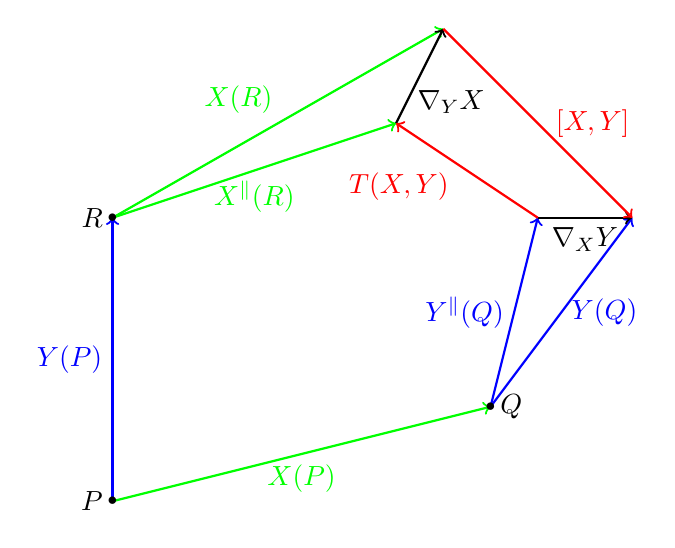
\begin{tikzpicture}[scale = 1.2]
                        \draw[->,thick,green] (0,0) -- (4,1) node[midway,below]{$X(P)$};
                        \draw[->,thick,green] (0,3) -- (3,4) node[midway,below]{$X^{\parallel}(R)$};
                        \draw[->,thick,green] (0,3) -- (3.5,5) node[midway,left=0.5cm,above]{$X(R)$};
                        \draw[->,thick,blue] (0,0) -- (0,3) node[midway,left]{$Y(P)$};
                        \draw[->,thick,blue] (4,1) -- (4.5,3) node[midway,left]{$Y^{\parallel}(Q)$};
                        \draw[->,thick,blue] (4,1) -- (5.5,3) node[midway,right]{$Y(Q)$};
                        \draw[->,thick] (4.5,3) -- (5.5,3) node[midway,below]{$\nabla_X Y$};
                        \draw[->,thick] (3,4) -- (3.5,5) node[midway,right=0.4cm,below=0.05cm]{$\nabla_Y X$};
                        \draw[->,thick,red] (3.5,5) -- (5.5,3) node[midway,right=0.1cm]{$[X,Y]$};
                        \draw[->,thick,red] (4.5,3) -- (3,4) node[midway,below=0.2cm  ,left=0.1cm]{$T(X,Y)$};
                        \draw (0,0) node[scale = 0.7]{$\bullet$};
                        \draw (4,1) node[scale = 0.7]{$\bullet$};
                        \draw (0,3) node[scale = 0.7]{$\bullet$};
                        \draw (0,0) node[below,left]{$P$};
                        \draw (4,1) node[below,right]{$Q$};
                        \draw (0,3) node[below,left]{$R$};
                    \end{tikzpicture}
                    \caption{Parallélogramme d'équipollence dans un espace courbe}
                \end{figure}
                
                En relativité générale, nous avons
                \begin{equation}
                    T^\mu_{\nu\rho} = \Gamma^\mu_{\nu\rho} - \Gamma^\mu_{\rho\nu}
                \end{equation}
                Et comme $\Gamma^\rho_{\mu\nu} = \Gamma^\rho_{\nu\mu}$, $T^\mu_{\nu\rho} = 0$. C'est-à-dire que c'est une connexion de torsion nulle.
                
            \subsection{Théorème fondamental de la géométrie riemanienne}
            
                Depuis le début du cours, nous avons écrit $\Gamma^\rho_{\mu\nu}$ pour les symboles de Christoffel, ceci a été fait en prédiction du résultat qui suit. Pour les symboles de Christoffel, la notation souvent utilisée est
                \begin{equation*}
                    \chris{\rho}{\mu}{\nu}\equiv
                    \Gamma^\rho_{\mu\nu}
                \end{equation*}
                et les symboles $\Gamma$ sont réservés à une connexion bien particulière qui est appellée la connexion de Levi-Civita. Nous allons voir que le théorème fondamentale de la géométrie riemannienne affirme que ces deux objets sont les mêmes. Toutefois, il est important de garder à l'esprit que ces deux objets ont a priori des origines différentes. Les symboles de Christoffel sont des coefficients qui apparaissent dans l'équation du mouvement d'une particule test. Ils sont définis comme
                \begin{equation}
                    \chris{\rho}{\mu}{\nu}~\hat{=}~
                    \frac{1}{2}g^{\mu\theta}\left( \p_\nu g_{\rho\theta}+\p_\rho g_{\nu\theta}-\p_\theta g_{\rho\nu} \right).
                \end{equation}
                Une connexion est une quantité qui porte la notion d'équipollence dans les espaces courbes. D'après les principes de la relativité générale, on peut imposer certaines conditions à la connexion que nous utilisons (préserve de la métrique $g$ et torsion nulle). La connexion de Levi-Civita est l'unique connexion qui satisfait ces conditions.\\
            
                \begin{thm}[fondamental de la géométrie riemannienne]\begin{leftbar}
                    Sur une variété riemannienne $(\M,g)$, il existe une unique connexion de torsion nulle préservant la métrique. On l'appelle la \textit{connexion de Levi-Civita} telle que
                    \begin{equation}
                        \chris{\rho}{\mu}{\nu}=\Gamma^\rho_{\mu\nu}
                    \end{equation}
                \end{leftbar}\end{thm}
                
                \begin{proof}${}$\\
                    Soit une variété $\M$ munie d'une métrique $g$ et considérons une connexion $\nabla$ sur le fibré tangent $T\M$.
                    Cette démonstration se fait en plusieurs étapes.
                    \begin{enumerate}[label = \textit{\roman*)}]
                            \item Montrons que la condition de connexion préservant la            métrique est équivalente à la condition
                                \begin{equation}
                                    \nabla_\mu g_{\nu\rho} = 0.
                                \end{equation}
                                Soient $3$ champs vectoriels sur $\M$ notés $X,Y$ et $V$. Si la connexion $\nabla$ préserve la métrique $g$, 
                                \begin{equation}
                                    \nabla_Vg(X,Y) = 0
                                \end{equation}
                                si $\nabla_V X = 0$ et $\nabla_V Y = 0$. Or de part la règle de Leibniz que nous avons déjà montrée,
                                \begin{align}
                                    0 &= \nabla_Vg(X,Y) \\
                                    &= V^\kappa \nabla_\kappa g(X,Y)\\
                                    &= V^\kappa(\nabla_\kappa g)(X,Y) + V^\kappa g( \nabla_\kappa X,Y) + V^\kappa g(X, \nabla_\kappa Y)\\
                                    &= V^\kappa(\nabla_\kappa g)(X,Y) + \underbrace{g(V^\kappa \nabla_\kappa X,Y)}_{0} +  \underbrace{g(X, V^\kappa\nabla_\kappa Y)}_{0}\\
                                    &= V^\kappa X^\mu Y^\nu \nabla_\kappa g_{\mu\nu}
                                \end{align}
                                Et particulier, si $V^\kappa = \delta^\kappa_\alpha,X^\mu = \delta^\mu_\beta$ et $Y^\nu = \delta^\nu_\sigma$, on obtient bien
                                \begin{equation}
                                    \nabla_\alpha g_{\beta\sigma} = 0.
                                \end{equation}
                                
                            \item Montrons que les coefficients $\Gamma^\rho_{\mu\nu}$ d'une connexion $\nabla$ compatible avec la métrique (i.e. qui préserve la métrique) sont donnés par 
                            \begin{equation}
                                \Gamma^\rho_{\mu\nu} = \chris{\rho}{\mu}{\nu}+
                                K\indices{_\mu^\rho_\nu}
                            \end{equation}
                            où
                            \begin{equation}
                                K\indices{_\mu^\rho_\nu} = \frac{1}{2}\left( T\indices{^\rho_\mu_\nu}+T\indices{_\mu^\rho_\nu} + T\indices{_\nu^\rho_\mu} \right)
                            \end{equation}
                            est appelé le \textit{tenseur de contorsion}. Au préalable, notons que 
                            \begin{align}
                                -\nabla_{\lambda}g_{\mu\nu} &= -\p_\lambda g_{\mu\nu}+\Gamma^\kappa_{\lambda\mu}g_{\kappa\nu}+\Gamma^\kappa_{\lambda\nu}g_{\mu\kappa}\\
                                \nabla_{\mu}g_{\lambda\nu} &= \p_\mu g_{\lambda\nu}-\Gamma^\kappa_{\mu\lambda}g_{\kappa\nu}-\Gamma^\kappa_{\mu\nu}g_{\lambda\kappa}\\
                                \nabla_{\nu}g_{\lambda\mu} &= \p_\nu g_{\lambda\mu}-\Gamma^\kappa_{\nu\lambda}g_{\kappa\mu}-\Gamma^\kappa_{\nu\mu}g_{\lambda\kappa}
                            \end{align}
                            Nous avons que si $\nabla$ préserve la métrique alors $\nabla_{\alpha}g_{\mu\nu} = 0$. En supposant que la métrique est bien conservée, nous avons donc
                            \begin{align}
                                 0 &=  -\nabla_{\lambda}g_{\mu\nu}+ \nabla_{\mu}g_{\lambda\nu}+ \nabla_{\nu}g_{\lambda\mu}\\
                                 &= \left(\Gamma^\kappa_{\lambda\mu}g_{\kappa\nu} -\Gamma^\kappa_{\mu\lambda}g_{\kappa\nu}\right) +\left(\Gamma^\kappa_{\lambda\nu}g_{\mu\kappa} -\Gamma^\kappa_{\nu\lambda}g_{\kappa\mu}\right)\\
                                 &\hspace{0.4cm}+\left(-\Gamma^\kappa_{\mu\nu}g_{\lambda\kappa}-\Gamma^\kappa_{\nu\mu}g_{\lambda\kappa}\right) + \left( -\p_\lambda g_{\mu\nu}+\p_\mu g_{\lambda\nu} + \p_\nu g_{\lambda\mu}\right)\\
                                 &= T^\kappa_{~\lambda\mu}g_{\kappa\mu}+T^\kappa_{~\lambda\nu}g_{\nu\kappa}-2\Gamma^\kappa_{~(\mu\nu)}g_{\lambda\kappa} + \left( -\p_\lambda g_{\mu\nu}+\p_\mu g_{\lambda\nu} + \p_\nu g_{\lambda\mu}\right)
                            \end{align}
                            Multiplions de chaque coté par $g^{\sigma\lambda}$ et notons que
                            \begin{equation} g^{\sigma\lambda}\Gamma^\kappa_{~(\mu\nu)}g_{\lambda\kappa} = \delta^\sigma_\kappa
                            \end{equation}
                            Ce qui permet d'obtenir l'expression suivante pour $\Gamma^\kappa_{~(\mu\nu)}$:
                            \begin{align}
                                \Gamma^\kappa_{~(\mu\nu)} &= \frac{1}{2}g^{\sigma\lambda}\left( -\p_\lambda g_{\mu\nu}+\p_\mu g_{\lambda\nu} + \p_\nu g_{\lambda\mu}\right)+\frac{1}{2}T^\kappa_{~\lambda\mu}g^{\sigma\lambda}g_{\kappa\mu}+\frac{1}{2}T^\kappa_{~\lambda\nu}g^{\sigma\lambda}g_{\nu\kappa}\\
                                &= \chris{\kappa}{\mu}{\nu}+\frac{1}{2}\left( T\indices{_\nu^\kappa_\mu}+T\indices{_\mu^\kappa_\nu} \right)\\
                                &= \chris{\kappa}{\mu}{\nu} + T\indices{_{(\nu}^\kappa_{\mu)}}
                            \end{align}
                            Enfin,
                            \begin{align}
                                 \Gamma^\sigma_{~\mu\nu} &=  \Gamma^\sigma_{~(\mu\nu)}+ \Gamma^\sigma_{~[\mu\nu]}\\
                                 &= \chris{\sigma}{\mu}{\nu} + T\indices{_{(\nu}^\sigma_{\mu)}} + \frac{1}{2}T^\sigma_{~\mu\nu}\\
                                 &=  \chris{\sigma}{\mu}{\nu}+\underbrace{\frac{1}{2}\left( T\indices{_\nu^\kappa_\mu}+T\indices{_\mu^\kappa_\nu} +T^\sigma_{\mu_\nu}\right)}_{K\indices{_\mu^\sigma_\nu}}
                            \end{align}
                        \item La dernière étape est de montrer l'unicité et l'existence grâce aux deux premières étapes. Soit une connexion $\nabla'$ sur $(\M,g)$ telle que $\nabla'g = 0$. Par l'étape précédente,
                        \begin{equation}
                        \widetilde{\Gamma}^\lambda_{\mu\nu}=\chris{\lambda}{\mu}{\nu}+K\indices{_\mu^\lambda_\nu}
                        \end{equation}
                        Définissons la connexion
                        \begin{equation}
                            \Gamma^\lambda_{\mu\nu} = \widetilde{\Gamma}^\lambda_{\mu\nu} + A^\lambda_{\mu\nu}.
                        \end{equation}
                        C'est bien une connexion à condition que $A^\lambda_{\mu\nu}$ soient les composantes d'un tenseur de type $(1,2)$. Supposons que le changement de coordonnées de $x$ à $x'$ se fait par l'intermédiaire que la matrice jacobienne $J$. Dans ce cas,
                        \begin{equation}
                            \Gamma' = J^{-1}JJ\Gamma + \text{anomalies}
                        \end{equation}
                        Nous utilisons bien une notation, il ne faut pas considérer le produit des matrices $J$ directement. De plus,
                        \begin{equation}
                            \widetilde{\Gamma}' = J^{-1}JJ\Gamma + \text{anomalies}
                        \end{equation}
                        où les "anomalies" sont les mêmes. Ceci implique que $\widetilde{\Gamma}-\Gamma$ est bien un tenseur car
                        \begin{equation}
                            (\widetilde{\Gamma}'-\Gamma') = J^{-1}JJ(\widetilde{\Gamma}-\Gamma).
                        \end{equation}
                        Il suffit de poser $A^\lambda_{\mu\nu}=-K\indices{_\mu^\lambda_\nu}$. Nous avons construit une connexion
                        \begin{equation}
                            \chris{\lambda}{\mu}{\nu}=\Gamma^\lambda{\mu\nu}
                        \end{equation}
                        qui est unique car $\chris{\rho}{\mu}{\nu}$ est défini univoquement à partir de la métrique.
                    \end{enumerate}
                \end{proof}
                
			Notons bien que de manière générale les symboles de connexion ne doivent pas s'écrire à partir de la métrique.         
                
                \begin{rmk}
                    On parle de géométrie riemannienne mais il s'agit en fait de géométrie pseudo-riemannienne car la variété de l'esapce-temps est munie d'une pseudo-métrique.
                \end{rmk}
                
                On conclu que le champ de gravitation est décrit par la métrique de l'espace-temps, c'est-à-dire par la géométrie de l'espace-temps.
            
        \section{Fibré vectoriel, section et connexion}
        
            \subsection{Section et fibre}
        
                Soit une variété différentiable $\M$. On veut généraliser la notion quantité physique (champ scalaire, champ vectoriel, champ tensoriel, champ spinoriel, etc). Prenons par exemple un champ scalaire. Il est claire que l'ensemble des valeur possible de champs doit former un espace vectoriel. Une quantité scalaire correspond donc en fait à une application sur l'espace-temps à valeur de $\mathbb{R}$. Ou de manière générale, une quantité physique est associée à une application dans un certain espace vectoriel.\\
                
                On voudrait associer à chaque point $P$ de $\M$, un espace vectoriel. Pour commencer, on se limite au cas particulier de l'esapce tangent.
                
                \begin{definition}
                    Le fibré tangent $T\M$ d'une variété différentiable $\M$ est l'ensemble
                    \begin{equation}
                        T\M = \bigcup_{P\in\M}T_P\M = \bigcup_{P\in\M}\left\{ (P,X)|P\in\M, X\in T_P\M \right\}
                    \end{equation}
                    muni de la projection
                    \begin{equation}
                    \pi:\left(
                    \begin{array}{ccc}
                        T\M & \longrightarrow & \M \\
                        (P,X) & \longmapsto & P
                    \end{array}
                    \right).
                    \end{equation}
                \end{definition}
                
                Une propriété remarquable du fibré tangent est qu'il lui-même être vu comme un variété.
                
                \begin{prop}\begin{leftbar}
                    Si $\M$ es une variété différentiable de dimension $n$ alors le fibré tangent $T\M$ admet une structure de variété différentiable de dimension $2n$ telle que
                    \begin{enumerate}[label = \textit{\roman*)}]
                        \item la projection $\pi:T\M\to\M$ est différentiable
                        \item chaque fibre $\pi^{-1}(P)$ est difféomorphe à $\mathbb{R}^n$ pour tout $P\in\M$
                    \end{enumerate}
                \end{leftbar}\end{prop}
                
                Le fibré tangent permet d'associer un espace vectoriel à chaque point de la variété, l'espace vectoriel est ici le cas particulier de l'espace tangent. L'espace tangent étant naturellement associé à un point de la variété cette notion est assez naturelle. On peut généraliser ce principe pour n'importe quel type d'espace vectoriel, plus seulement l'espace tangent. On appelle ca le fibré vectoriel.
                
                \begin{definition}
                    Un \textit{fibré vectoriel} réel $\F$ de dimension $k$ sur la variété différentiable $\M$ est de projection $\pi:\F\to\M$ est une variété différentiable telle que pour tout $P\in\M$ il existe un voisinage $U\subset\M$ autour de $P$ tel que $\pi^{-1}(U)$ est difféomorphe à $U\times \mathbb{R}^k$ avec les propriétés suivantes
                    \begin{enumerate}[label = \textit{\roman*)}]
                        \item le diagramme suivant commute
                        \begin{center}
                            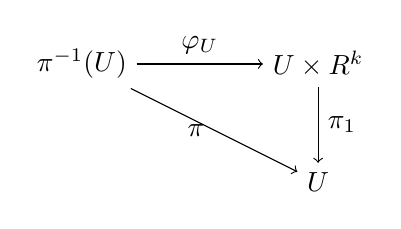
\begin{tikzpicture}
                                \node (A) at (0,0) {$\pi^{-1}(U)$};
                                \node (B) at (3,0) {$U\times\mathbb{R}^k$};
                                \node (C) at (3,-1.5) {$U$};
                                \draw[->] (A) -- (B) node[midway, above]{$\varphi_U$};
                                \draw[->] (B) -- (C) node[midway, right]{$\pi_1$};
                                \draw[->] (A) -- (C) node[midway, left]{$\pi$};
                            \end{tikzpicture}
                        \end{center}
                        où $\varphi_U$ est un difféomorphisme et $\pi_1$ est la projection sur le premier facteur.
                        \item toute composition $\varphi_V\circ\varphi_U^{-1} : (U\cap V)\times \mathbb{R}^k\to (U\cap V)\times \mathbb{R}^k$ où $U$ et $V$ sont disjoints, est linéaire en le second facteur.
                    \end{enumerate}
                \end{definition}
                
                La première propriété a pour but d'assurer que la projection $\pi:\F\to\M$ est différentiable. La seconde propriété implique que la structure d'espace vectoriel est conservée par les applications $\varphi_V\circ\varphi_U^{-1}$. On peut voir $\F$ comme une famille d'espaces vectoriels réels de dimension $k$ paramétrisée par $\M$.\\
                
                \begin{definition}
                    L'espace vectoriel qui est associé à un point $P\in\M$ est appelé la \textit{fibre} en ce point. L'ensemble des fibres forme donc le fibré vectoriel.
                \end{definition}
                
                \begin{definition}
                    Soit un fibré vectoriel $\F$ de projection $\pi:\F\to\M$. Une \textit{section} de ce fibré vectoriel est une application différentiable $s:M\to\F$ telle que $\pi\circ s = id$ sur $\M$.
                \end{definition}
                
                On peut définir plus rigoureusement toute une série de termes.
                \begin{definition}${}$
                    \begin{itemize}[label = \textbullet]
                        \item un \textit{champ scalaire} est une section pour $\F = \mathbb{R}$
                        \item un \textit{champ vectoriel} est une section du fibré tangent
                        \item un \textit{champ tensoriel} est une section pour $\F = T_P^{(p,q)}\M$.
                        \item un \textit{champ de $1$-formes} est une section pour $\F = \Omega^1(\M)$
                    \end{itemize}
                \end{definition}
                
                Notons que ce formalisme n'est pas valable que pour la relativité générale mais aussi dans d'autres théories.
                
                \begin{exmp}${}$
                    \begin{itemize}[label = \textbullet]
                        \item mécanique quantique : $\F_P = \mathbb{C}$ et les sections sont les fonctions d'onde
                        \item modèle standard des interactions fondamentales : les sections sont des champs quantiques de matière
                    \end{itemize}
                \end{exmp}
                
                \begin{definition}
                    Un \textit{fibré principal} est un fibré qui est aussi un groupe.
                \end{definition}
                
                Dans notre cas nous aurons souvent $\F_P = T_P^{(p,q)}\M$ mais les discussions qui suivent ne dépendent pas de ce choix.\\
                
                Notons que les fibres existent indépendemment de $\M$. Pour tout point $P\in\M$, on peut toujours se donner une base $\{e_a(P)\}$ de $\F_P$. De cette manière, $s(P)$ peut être développés sur cette base comme
                \begin{equation}
                    s(P) = s^a(P)e_a.
                \end{equation}
                Si on a une matrice de changement de base $M$ qui permet de passer de la base $\{e_a(P)\}$ à une nouvelle base $\{e'_a(P)\}$ comme $e_a = M^b_{~~a} e'_b$, alors
                \begin{equation}
                    s'^a = M^a_{~~b}s^b
                \end{equation}
                
                Ce genre de transformation peut changer la forme des loi de la physique mais la physique en tant que telle reste la même. On sous-entend par là que comme les lois de la physique dépendent des sections elle-mêmes mais pas de la manière dont on écrit ces sections. Pour pouvoir décrire une section, il faut spécifier une base mais ce choix ne joue aucun rôle fondamental. On a discuté l'exemple d'un changement de base dans $\F_P$, ce qui correspond en fait à un changement de référentiel, mais on peut en fait s'autoriser toute une série de transformations plus générale encore cela.
                
                \begin{definition}
                    Soit $\{e_a(P)\}$ une base de $\F_P$ et $s = s^a(P)e_a$ une section, on appelle \textit{transformation de jauge} les transformations de type
                    \begin{equation}
                    s'^a = M^a_{~~b}s^b
                    \end{equation}
                    où $M\in G\subset GL(dim(\F_P),\mathbb{R})$. $G$ est appelé le \textit{groupe de structure du fibré} (ou \textit{groupe de jauge}).
                \end{definition}
                
                Les transformations de jauge décrivent les fameuse symétries de jauge qui, comme nous l'avons mentionné précédemment, ne sont en fait pas des symétries à proprement parlé.
                
                \begin{exmp}
                    Prenons un exemple en mécanique quantique. On a $\F_P = \mathbb{C}$ et $G = U(1)$. Soit une fonction d'onde $\psi|_P$ en $P$, la fonction d'onde
                    \begin{equation}
                        \psi'|_P = e^{i\alpha}\psi|_P
                    \end{equation}
                    est alors équivalent pour tout $\alpha\in\mathbb{R}$.
                \end{exmp}
                
                Pour reformuler, en chaque point de l'espace-temps, on a un espace vectoriel qui contient les quantités physiques. Sur cet espace vectoriel, on s'autorise des transformations de jauge. Par exemple, le fait d'écrire un vecteur dans une base ou dans une autre ne change rien: le vecteur a une existence intrinsèque, indépendante du choix de la base. Les transformations de jauge implémentent cette redondance.
            
            \subsection{Dérivation de section}
            
                Maintenant que ces notions sont établies, il est nécessaire de définir une notion de dérivée pour les sections. Soit $s$ une section, alors si $P,Q\in\M$, on pourrait être tenter de définir
                \begin{equation}
                    \nabla_\mu s~ dx^\mu = s(Q)-s(P)
                \end{equation}
                 mais $s(P)\in\F_P$ et $s(Q)\in\F_Q$ et soustraire des vecteurs qui ne sont pas au même point n'a pas de sens. En géométrie euclidienne ce problème n'existe pas car l'équipollence des vecteurs permet de pouvoir ramener n'importe quels vecteurs au même point. Comme l'espace de la géométrie euclidienne est plat, les vecteurs ne changent pas quand on les translate. Dans notre cas, il faut tenir compte de la courbure de l'espace pour pouvoir transformer les vecteurs correctement quand on les ramènes au même point, c'est ce rôle que joue les symboles de connexion. Considérons une sphère et deux vecteurs $v_1$ et $v_2$ et deux points différent cette sphère. Pour pourvoir soustraire ces vecteurs, il faut ramener $v_2$ au même point que $v_1$ (ou l'inverse). Si l'on fait juste une translation de $v_2$ on perd les propriétés du vecteurs. Par exemple, si $v_2$ est tangent à la sphère, le vecteur résultant ne le sera plus. Il faut adapté la notion de translation sur la sphère en tenant compte de la courbure. S'il on connaît comment s'exprime un vecteur "bien translaté" en fonction du vecteur d'origine dans une base donnée c'est bon. Les coefficients de la combinaison linéaire jouerais le rôle de connexion (symboles de connexion). Il est clair que ces symboles sont intrinsèque à la surface considérée, ici la sphère. L'idée est la même pour l'espace-temps. En d'autres termes, cet exercice de transport parallèle dans l'espace-temps doit être fait pas un certain isomorphisme. Il faut donc se donner un isomorphisme entre fibres $\F_P$ et $\F_Q$ "proches" (lorsque $P$ et $Q$ sont proches). Cet isomorphisme donnera la notion de transport parallèle. Faisons une tentative.
                 
                 \begin{definition}
                    Soit $\S_{P\to Q}$ l'\textit{opérateur de transport parallèle infinitésimal} un isomorphisme entre $\F_P$ et $\F_Q$.
                 \end{definition}
                 
                 D'après le raisonnement expliqué précédemment, on a alors
                 \begin{equation}\label{eq:derivsec}
                     \nabla_\mu s^a~dx^\mu = s^a(Q)-\left(\S_{P\to Q}(P)\right)^a
                 \end{equation}
                 et, par définition de dérivée covariante, on obtient
                 \begin{align}
                     \left(\S_{P\to Q}(P)\right)^a &= s^a(Q) + \nabla_\mu s^a~dx^\mu\\
                     &= s^a(Q) - \Gamma^a_{\mu b}~ s^b(P) ~dx^\mu
                 \end{align}
                 Si l'on utilise la notation $\Gamma_\mu$ pour le tenseur d'ordre deux de composantes $\Gamma^a_{\mu b}$, 
                 \begin{equation}
                     \S_{P\to Q}(P) = \mathbb{1} - \Gamma_\mu~dx^\mu
                 \end{equation}
                 Pour finir, s'il on prend $P = x$ et $Q = x+dx$, l'équation \ref{eq:derivsec} devient
                 \begin{align}
                      \nabla_\mu s^a~dx^\mu &= s^a(x+dx)-\left(\S_{P\to Q}(x)\right)^a\\
                      &= s^a(x+dx)-s^a(x)+\Gamma^a_{\mu b}s^b~dx^\mu
                 \end{align}
                 et donc lorsque $dx\to0$,
                 \begin{equation}
                     \nabla_\mu s^a = \p_\mu s^a+\Gamma^a_{\mu b}s^b.
                 \end{equation}
                 On voit bien que les $\Gamma^a_{\mu b}$ portent la notion d'équivalence de vecteur pour un espace courbe de métrique $g$. \\
                 
                 Après cette approche intuitive, voyons maintenant une approche plus axiomatique de la même notion.
                 
                 \begin{definition}
                    On note $\Sigma^p$ l'espace des $p$-formes à valeur dans les sections.
                 \end{definition}
                 
                 Notons que, d'après cette définition, $\Sigma^0$ est l'espace des sections elles-mêmes. Nous avons donc
                 \begin{equation}
                    \Sigma^p = \Omega^p(\M)\otimes\Sigma^0.
                \end{equation}
                
                \begin{exmp}
                    Soit $h\in \Sigma^p$, alors
                    \begin{equation}
                        h = \frac{1}{p!}\omega^a_{\mu_1\dots\mu_p}~dx^{\mu_1}\wedge\dots\wedge dx^{\mu_p}\otimes e_a.
                    \end{equation}
                    
                    Si $p=1$, $h\in\Sigma^1$ et si $x\in T_P\M$ alors $h(x)\in\Sigma^0$ car 
                    \begin{equation}
                        h = h^a_\mu~dx^\mu\otimes e_a
                    \end{equation}
                    et donc
                    \begin{equation}
                        h(x) = h^a_\mu x^\mu e_a.
                    \end{equation}
                \end{exmp}
                
                \begin{definition}
                    Une \textit{connexion} est une application
                    \begin{equation}
                    \nabla:\left(
                    \begin{array}{ccc}
                        \Sigma^0 & \longrightarrow & \Sigma^1 \\
                        f & \longmapsto & \nabla f
                    \end{array}
                    \right)
                    \end{equation}
                    telle que 
                    \begin{equation}
                        \nabla(fs) = df\otimes s+f\nabla s
                    \end{equation}
                    pour toute fonction $f:\M\to\mathbb{R}$ et pour tout $s\in\Sigma^0$.
                \end{definition}
                
                Notons que $\nabla$ est à valeur dans $\Sigma^1$ var la dérivation est fonctionnelle. Si $S\in T_P\M$,
                \begin{align}
                    \nabla_X s &= (\nabla s)(X)\\
                    &= X^\mu(\nabla s)(\p_\mu)\\
                    &= X^\mu\nabla_\mu s
                \end{align}
             
                Soit $\{e_a^{(P)}\}$ une base de $\F_P$ alors
                \begin{align}
                    \nabla s &= \nabla(s^a e_a)\\
                    &= ds^a\otimes e_a+s^a\nabla e_a
                \end{align}
            donc $\nabla s$ est fixée, quelque soit $s$, si l'on connaît $\nabla e_a$. 
            \begin{definition}
                Les \textit{$1$-forme de la connexion} sont les  $1$-forme $\Gamma^b_a\in\Omega^1(\M)$ à valeur dans l'espace des sections qui permettent la décomposition
                \begin{equation}
                    \nabla e_a = \Gamma^b_a \otimes e_b.
                \end{equation}
                On note $\Gamma$ la matrice des $1$-forme de la connexion.
             \end{definition}
             
            D'après ce que l'on a vu ci-dessus,
            \begin{equation}
                 \Gamma^a_b = \Gamma^a_{\mu b}~dx^\mu
            \end{equation}
            on voit bien que les indices $a,b$ et $\mu$ jouent des rôles très différents. Finalement, nous retrouvons la même formule que dans notre approche intuitive du problème.
            \begin{align}
                 \nabla s(X) &= \nabla_X s\\
                 &= ds^a(X)e_a+\Gamma^a_b(X)e_b\\
                 &= X^\mu(\p_\mu s^a+\Gamma^a_{\mu b}s^b)e_a
            \end{align}
             
            \begin{prop}\begin{leftbar}
                    La dérivée covariante d'une section $s = s^a e_a$ est donnée par
                    \begin{equation}
                        \nabla_\mu s^a = \p_\mu s^a+\Gamma^a_{\mu b}s^b
                    \end{equation}
            \end{leftbar}\end{prop}
             
            Que se passe-t-il sous un changement de base ? Ou de manière plus générale, que se passe-t-il sous une transformation de jauge ? Pour faire le cas générale, on va considérer un changement de base uniquement pour les fibres et pas dans l'esapce tangent. On verra plus après le cas particulier où les fibres sont des espaces tangents qu'est le notre.
            
            \begin{prop}\begin{leftbar}
                Sous un changement de coordonnées du type
                \begin{align}
                    e_a' &= N_a^{~b}~e_b \\
                    s'^a &= M^a_{~b} ~s^b
                \end{align}
                 avec $M\in G$ et $N = (M^{-1})^T$. Nous avons
                 \begin{equation}
                     \Gamma' = M\Gamma M^{-1} + MdM^{-1}
                 \end{equation}
            \end{leftbar}\end{prop}
        
            \begin{proof}
                On a 
                \begin{equation}
                    (\nabla s)^a = ds^a + \Gamma^a_b s_b.
                \end{equation}
                D'une part, 
                \begin{align}
                    (\nabla s)'^a &= ds'^a +  \Gamma'^a_{~b} s'_b \\
                    &= d(M^a_{~b} ds^b) + \Gamma'^a_{~b} M^b_{~c}s^c \\
                    &= M^a{~b}ds^b + dM^a_{~c}s^b + \Gamma'^a_{~b} M^b_{~c}s^c
                \end{align}
                et d'autre part,
                \begin{align}
                    (\nabla s)'^a &= M^a_{~b}(\nabla s)^b \\
                    &=  M^a_{~b}\left( ds^b+\Gamma^b_{~c}s^c \right)
                \end{align}
                ce qui entraîne que
                \begin{align}
                     M^a_{~b}\Gamma^b_{~c}s^c &=  dM^a_{~c}s^b + \Gamma'^a_b M^b_{~c}s^c\\
                     \Leftrightarrow \qquad (M\Gamma)^a_{~c}s^c &= dM^a_{~c}s^b + (\Gamma'M)^a_{~c}s^c\\ 
                     \Leftrightarrow \qquad M\Gamma &= \Gamma'M - dM
                \end{align}
                ou encore
                \begin{align}
                    \Gamma' &= M\Gamma M^{-1}-(dM)M^{-1}\\
                    &= M\Gamma M^{-1} + MdM^{-1}
                \end{align}
                Le dernière égalité venant du fait que $MM^{-1} = \mathbb{1}$ et donc 
                \begin{equation}
                    dM\cdot M^{-1} + M\cdot dM^{-1} = 0.
                \end{equation}
            \end{proof}
        
            Remarquons que, composante par composante, la loi de transformation des $\Gamma$ donne 
            \begin{equation}
                \Gamma'^{a}_{~b} = M^a_{~c}\Gamma^c_{~d}(M^{-1})^d_{~b}+M^a_{~c}(dM^{-1})^c_{~b}
            \end{equation}
            ce qui montre bien que $\Gamma$ n'est pas une $1$-forme à valeur dans $F\otimes F^* = End(F)$.
            \begin{equation}
                \Gamma\notin \Omega^1(\M)\otimes F \otimes F^*
            \end{equation}
            Toujours d'après ce que l'on vient de voir, si $\Gamma = \Gamma_\mu~dx^\mu$,
            \begin{equation}
                \Gamma'_{\mu} = M\Gamma M^{-1} + M\p_\mu M^{-1}.
            \end{equation}
            Notons bien que nous avons effectué un changement de base sur la fibre mais que nous avons utilisé la même base de $\Omega^1(\M)$ pour développer $\Gamma'$ et $\Gamma$.\\
            
            Dans le cas particulier où $F_P : T_P\M$ et où le changement de base sur la fibre correspond à un changement de coordonnées, il est naturelle d'exprimer les $1$-forme $\Gamma$ dans la base $\{dx^\mu\}$ et les $1$-formes $\Gamma'$ dans la base $\{dx'^\mu\}$. Dans ce cas, $M^a_{~b}$ devient $\pdv{x'^\mu}{x^\nu}$ et donc 
            \begin{equation}
                \gamma'^\mu_{~\nu} = \pdv{x'^\mu}{x^\rho}\pdv{x^\sigma}{x^\nu}\Gamma^\rho_{~\sigma} + \pdv{x'^\mu}{x^\theta}~d\left( \pdv{x^\theta}{x'^\nu} \right)
            \end{equation}
            On exprime $\Gamma$ et $\Gamma'$ comme suit.
            \begin{equation}
                \Gamma'^\mu_{~\nu} =  \Gamma'^\mu_{\kappa\nu}~dx'^\kappa \qquad ; \qquad  \Gamma^\rho_{~\sigma} =  \Gamma^\rho_{\xi\sigma}~dx^\xi
            \end{equation}
            On trouve donc 
            \begin{align}
                \Gamma'^\mu_{\kappa\nu}~dx'^\kappa &= \pdv{x'^\mu}{x^\rho}\pdv{x^\sigma}{x^\nu} \Gamma^\rho_{\xi\sigma}~dx^\xi + \pdv{x'^\mu}{x^\theta}\pdv{x^\theta}{x'^\nu}{x'^\kappa}~dx'^\kappa\\
                &= \pdv{x'^\mu}{x^\rho}\pdv{x^\sigma}{x^\nu} \Gamma^\rho_{\xi\sigma}\pdv{x^\xi}{x'^\kappa}~dx^\kappa + \pdv{x'^\mu}{x^\theta}\pdv{x^\theta}{x'^\nu}{x'^\kappa}~dx'^\kappa
            \end{align}
            En identifiant les coefficients devant les $dx'^\kappa$, on retrouve la loi de transformation de $\Gamma$.
            
            \begin{exmp}
                Si $G = U(1)$ et $F = \mathbb{C}$, alors $M = e^{i\alpha}$ et $\Gamma$ est une matrice $1\times1$ et donc
                \begin{align}
                    \Gamma' &= M\gamma M^{-1} + MdM^{-1} \\
                    &= \Gamma + e^{i\alpha}d(e^{i\alpha}) \\
                    &= \Gamma-i\alpha d\alpha
                \end{align}
                Dans une base des coordonnées,
                \begin{equation}
                    \Gamma'_\mu = \Gamma_\mu-i\alpha\p_\mu\alpha
                \end{equation}
                Dans le cas du potentiel vecteur électromagnétique, on trouve la transformation de jauge
                \begin{equation}
                    A'_\mu = A_\mu - \p_\mu\alpha.
                \end{equation}
                Et, 
                \begin{align}
                    \nabla_\mu\psi &= \p_\mu\psi + \Gamma_\mu \\
                    &= (\p_\mu+iA_\mu)\psi
                \end{align}
                C'est la dérive covariante d'un spinneur chargé. On verra que dans ce cas, la courbure est le champ électromagnétique. Le potentiel vecteur est à l'électromagnétisme ce que $\Gamma$ est à la relativité générale.
            \end{exmp}
            
            \begin{exmp}
                Dans le modèle standard des interactions fondamentales, $G$ est un groupe non-abélien :
                \begin{equation}
                    G = SU(3)\times SU(2)\times U(1)
                \end{equation}
                et $\Gamma = iA$ (c'est un élément de l'algèbre de Lie de $G$). Dans ce cas, on trouve
                \begin{equation}
                    A' = MAM^{-1}-iMdM^{-1}.
                \end{equation}
                C'est la transformation de jauge pour une théorie de jauge non-abélienne.
            \end{exmp}
        
        \section{Lignes droites et géodésiques}
        
            \begin{definition}
                Soit $(I,\gamma)$ une courbe $C^\infty$ dans $\M$, $I$ est  un intervalle ouvert de $\mathbb{R}$ et $\gamma:I\to\M$ une application $C^\infty$. Pour tout $\lambda\in I$, on définit un vecteur tangent à $\M$ au point $\gamma(\lambda)$, appelé \textit{vecteur tangent à la courbe} $\gamma$ en $\lambda$, on le note $\dot{\gamma}(\lambda)$.
                \begin{equation}
                    \dot{\gamma}:\left(
                    \begin{array}{ccc}
                        C^\infty(\M,\mathbb{R}) & \longrightarrow & \mathbb{R} \\
                        f & \longmapsto & \dot{\gamma}(\lambda)(f)
                    \end{array}
                    \right)
                    \end{equation}
                    où
                    \begin{equation}
                         \dot{\gamma}(\lambda)(f) ~\hat{=}~ \frac{d}{dt}f(\gamma(t))|_{t=\lambda}.
                    \end{equation}
            \end{definition}
            
            On voit bien que c'est un vecteur de l'espace tangent car $f\circ\gamma$ est une fonction $C^\infty$ et la dérivée $\frac{d}{dt}$ satisfait à la règle de Leibniz.
            
            \begin{rmk}
                Lorsque l'on a introduit la notion d'espace tangent, on a montré que les dérivée partielle en fonction des dérivées locales formaient une base de ce dernier. Cela veut dire qu'il est possible de développer l'expression d'un vecteur tangent à une courbe sur cette base. Cela se fait en faisant apparaître l'application de coordonnée dans l'expression puis en utilisant la chain rule. On peut montrer que tout vecteur tangent $X_P\in T_P\M$ en $P$ peut être considéré comme un vecteur tangent à une courbe passant par $P$. Cette caractérisation est non unique.
            \end{rmk}
            
            Nous noterons $x^\mu(\lambda)\equiv (x\circ \gamma)(\lambda)$ une courbe dans $\M$ de paramètre $\lambda$. Le vecteur tangent à cette courbe en $P$ est
                \begin{equation}
                    U^\mu = \frac{dx^\mu}{d\lambda}(P)
                \end{equation}
            ce n'est donc pas un champ de vecteur comme on l'a vu avant car ces vecteurs sont définis uniquement le long de la courbe. On vérifie facilement que c'est bien un vecteur.\\
            
            Comme $U^\mu$ n'est défini que le long de la courbe, la dérivée covariante $\nabla_X U^\mu\equiv X^\nu\nabla_\nu U^\mu$ n'est pas bien définie. On peut cependant définir correctement $\nabla_U U^\mu\equiv U^\nu\nabla_\nu V^\mu$. Nous avons alors
            \begin{align}
                \nabla_U U^\mu &= U^\nu\nabla_\nu U^\mu \\
                &= \frac{dx^\nu}{d\lambda}\p_\nu U^\mu + \Gamma^\mu_{\nu\rho}U^\nu U^\rho \\
                &= \frac{d^2x^\mu}{d\lambda^2} + \Gamma^\mu_{\nu\rho} \frac{dx^\nu}{d\lambda}\frac{dx^\rho}{d\lambda}
            \end{align}
            Ce résultat peut être généralisé à n'importe que tenseur défini le long d'une courbe $\mathscr{C}$.
            \begin{prop}\begin{leftbar}
                Soit une courbe $\mathscr{C}$ sur $\M$ de paramètre $\lambda$. Si $U$ est un vecteur tangent à $\mathscr{C}$, alors la dérivée d'un tenseur $t$ de type $(p,q)$ est
                \begin{equation}
                    \nabla_U t^{\mu_1\dots\mu_p}_{\nu_1\dots\nu_q} = \frac{dt^{\mu_1\dots\mu_p}_{\nu_1\dots\nu_q}}{d\lambda} + U^\mu(\Gamma_\mu t + \dots)
                \end{equation}
            \end{leftbar}\end{prop}
            
            \begin{proof}
                Il suffit de développer l'expression de la dérivée covariante de la même manière que précédemment.
            \end{proof}
            
            Les tenseurs $\nabla t$ sont définit le long de $\mathscr{C}$.\\
            
            Comment définir une ligne droite ? En géométrie euclidienne, la droite peut être définie comme étant le plus court chemin entre deux points. Cependant, la notion "plus court" dépend de la métrique dont dispose l'espace que l'on étudie. Le fait que le chemin le plus court entre deux points est une droite est une conséquence de la forme de la métrique euclidienne. Sur une sphère, les chemins les plus court sont des les grands cercles. Fondamentalement, on peut définir une droite comme étant une courbe dont le vecteur tangent ne change pas de direction. C'est-à-dire une courbe telle que
            \begin{equation}
                \nabla_U U = f(\lambda) U
            \end{equation}
            Notons que ceci a bien du sens car $\nabla_\mu U\in T^{(1,1)}\M$ et donc $\nabla_U U = U^\mu\nabla_\mu U\in T^{(1,0)}\M$. La notion de ligne droite dépend de la connexion de transport parallèle.\\
            
            Le membre de droite peut toujours être éliminé par un choix approprié de paramètre $\lambda$. Effectivement, supposons que $\lambda = \lambda(\lambda')$,
            \begin{align}
                \nabla_U U^\mu &= \frac{dU^\mu}{d\lambda} + \Gamma^\nu_{\mu\rho} U^\mu U^\rho \\
                &= \frac{d^2x^\mu}{d\lambda^2} + \Gamma^\nu_{\mu\rho} \frac{dx^\nu}{d\lambda}\frac{dx^\mu}{d\lambda} \\
                &= \left( \frac{d\lambda'}{d\lambda} \right)^2\frac{d^2x^\mu}{d\lambda'^2}+\frac{d^2\lambda'}{d\lambda^2}\frac{dx^\mu}{d\lambda'}+\left( \frac{d\lambda'}{d\lambda} \right)^2\Gamma^\mu_{\nu\rho} \frac{dx^\nu}{d\lambda'}\frac{dx^\mu}{d\lambda'}
            \end{align}
            d'autre part, 
            \begin{align}
                \nabla_U U^\mu &= f(\lambda) \frac{dx^\mu}{d\lambda} \\
                &= \frac{d\lambda'}{d\lambda}f(\lambda)\frac{dx^\mu}{d\lambda'}
            \end{align}
            En égalant ces deux termes, on trouve
            \begin{equation}
                \left( \frac{d\lambda'}{d\lambda} \right)^2\frac{d^2x^\mu}{d\lambda'^2}+\frac{d^2\lambda'}{d\lambda^2}\frac{dx^\mu}{d\lambda'}+\left( \frac{d\lambda'}{d\lambda} \right)^2\Gamma^\mu_{\nu\rho} \frac{dx^\nu}{d\lambda'}\frac{dx^\mu}{d\lambda'} = \frac{d\lambda'}{d\lambda}f(\lambda)\frac{dx^\mu}{d\lambda'}
            \end{equation}
            donc
            \begin{equation}
                \frac{d^2x^\mu}{d\lambda'^2} + \Gamma^\mu_{\nu\rho} \frac{dx^\nu}{d\lambda'}\frac{dx^\mu}{d\lambda'} = 0
            \end{equation}
            si et seulement si
            \begin{align}
                \frac{d^2\lambda'}{d\lambda^2} &= \frac{d\lambda'}{d\lambda}f(\lambda)
            \end{align}
            et cette équation différentielle est toujours solvable. Il existe toujours une solution $\lambda'(\lambda)$.
            
            \begin{definition}
                Le paramètre permettant de réduire l'équation d'une droite à 
                \begin{equation}
                    \nabla_U U = 0
                \end{equation}
                est appelé \textit{paramètre affine}.
            \end{definition}
            
            \begin{prop}\begin{leftbar}
                Soient $\lambda_1$ et $\lambda_2$ deux paramètres affines d'une courbe $\mathscr{C}$. Il existe $\alpha,\beta\in\mathbb{R}$ tels que
                \begin{equation}
                    \lambda_1 = \alpha\lambda_2+\beta.
                \end{equation}
            \end{leftbar}\end{prop}
            
            \begin{proof}
                Nous avons vu que si $\lambda'$ et $\lambda$ sont des paramètres affines alors
                \begin{equation}
                    \frac{d^2\lambda'}{d\lambda^2} = 0
                \end{equation}
                ce qui implique bien que
                \begin{equation}
                    \lambda' = \alpha \lambda + \beta
                \end{equation}
                pour $\alpha,\beta\in\mathbb{R}$.
            \end{proof}
            
            Pour certaines courbes, le paramètre affine correspond à une quantité physique bien connue : le temps propre.
            
            \begin{definition}
                Une \textit{géodésique} est une courbe qui extrémalise la distance entre deux point.
            \end{definition}
            
            \begin{exmp}
                En géométrie euclidienne, la distance entre deux points $P$ et $Q$ est donnée par 
                \begin{equation}
                    L = \int_P^Q ds = \int_P^Q \sqrt{dx^2+dy^2}
                \end{equation}
                on peut alors montrer que les courbes satisfaisant $\delta L = 0$ sont les lignes droites.
            \end{exmp}
            
            \begin{exmp}
                Sur la sphère unité $S^2$, la distance est donnée par
                \begin{equation}
                    L = \int_P^Qds = \int_P^Q\sqrt{dr^1+d\theta^2+\sin^2\theta d\phi^2}
                \end{equation}
                en coordonnées sphériques. Les courbes qui extrémalisent cette distance sont les grands cercles (cercle issus de l'intersection d'un plan passant par le centre avec la sphère). Dans le cas de la Terre par exemple, il n'est en effet pas possible de marcher tout droit sans se déplacer sur un grand cercle. L'expression "marcher tout droit" signifiant marcher sans changer sa direction dans ce cas-ci (vecteurs tangents co-linéaires). On voit que les géodésiques sont l'équivalent (ou la généralisation) des lignes droites dans les espaces euclidiens.
            \end{exmp}
            
            \begin{definition}
                En signature Minkowskienne, on considère 3 types de courbe :
                \begin{itemize}[label = \textbullet]
                    \item de \textit{genre temps} : si $g(U,U)<0$
                    \item de \textit{genre lumière} : si $g(U,U)=0$
                    \item de \textit{genre espace} : si $g(U,U)>0$
                \end{itemize}
            \end{definition}
            
            \begin{exmp}
                En relativité restreinte, la distance est donnée par
                \begin{equation}
                    S = -m\int_P^Qd\tau = -m\int_P^Q\sqrt{\eta_{\alpha\beta}dx^\alpha dx^\beta} = -m\int_P^Q\sqrt{1-v^2}dt
                \end{equation}
                où le signe "-" et le paramètre $m$ (masse) sont conventionnels. Les courbe qui minimisent la distance sont celles qui minimisent l'action $S$, c'est-à-dire les courbe pour lesquelles $v=0$.
            \end{exmp}
            
            \begin{thm}\begin{leftbar}
                Si $\Gamma$ est la connexion de Levi-Civita alors les lignes droites extrémalisent  la fonctionnelle temps propre entre deux points
                \begin{equation}
                    S = -m\int_P^Qd\tau
                \end{equation}
                pour les courbes de genre temps.
            \end{leftbar}\end{thm}
            
            \begin{proof}${}$\\
                Rappelons que, par définition du temps propre,
                \begin{align}
                    S &= -m\int_P^Q d\tau\\
                    &= -m\int_{\lambda_1}^{\lambda_2}\sqrt{-g_{\mu\nu}\dot{x}^\mu\dot{x}^\nu}d\lambda
                \end{align}
                où $\dot{x}^\mu = \frac{x^\mu}{d\lambda}$. Nous avons le lagrangien
                \begin{equation}
                    \mathcal{L} = \sqrt{-g_{\mu\nu}\dot{x}^\mu\dot{x}^\nu}.
                \end{equation}
                Il suit que
                \begin{align}
                    \pdv{\mathcal{L}}{x^\mu} &= -\frac{2}{\sqrt{2F}}\p_\mu g_{\nu\rho}\dot{x}^\mu\dot{x}^\nu \\
                    \pdv{\mathcal{L}}{\dot{x}^\mu} &= -\frac{2}{2\sqrt{F}}g_{\mu\nu}\dot{x}^\nu\\
                    \frac{d}{d\lambda}\pdv{\mathcal{L}}{\dot{x}^\mu} &= -\frac{g_{\mu\nu}\ddot{x}^\nu}{\sqrt{F}}-\frac{\p_\mu g_{\mu\nu} \dot{x}^\mu\dot{x}^\nu}{\sqrt{F}}-\frac{1}{2F^{\frac{3}{2}}}\frac{dF}{d\lambda}
                \end{align}
                Les équation d'Euler-Lagrange nous donnent alors
                \begin{equation}
                    \ddot{x}^\xi + \underbrace{\frac{1}{2}g^{\mu\xi}\left( \p_\rho g_{\mu\nu}+\p_\nu g_{\mu\rho} - \p_\mu g_{\nu\rho} \right)}_{\Gamma^\xi_{\nu\rho}}\dot{x}^\nu\dot{x}^\rho = f(\lambda)
                \end{equation}
                ou encore
                \begin{equation}
                    \nabla_U U^\mu = f(\lambda)U^\mu
                \end{equation}
            \end{proof}
            
            Notons que si l'on prend $\lambda = \tau$, alors $g(U,U) = -1 = -F$ et donc
            \begin{equation}
                \frac{dF}{d\lambda} = 0.
            \end{equation}
            On peut en conclure que le temps propre est un paramètre affine. En géométrie euclidienne, l'abscisse curviligne est un paramètre affine.
            
            \begin{prop}\begin{leftbar}
                Si $U$ est le vecteur tangent le long d'un courbe, alors la quantité
                \begin{equation}
                    g(U,U) = g_{\mu\nu}U^\mu U^\nu
                \end{equation}
                où $U^\mu = \frac{dx^\mu}{d\lambda}$, est constante le long de cette courbe.
            \end{leftbar}\end{prop}
            
            \begin{proof}${}$\\
                Il suffit de remarquer que
                \begin{align}
                    \frac{d}{d\lambda}\left((g(U,U)\right) &= \frac{dx^\mu}{d\lambda}\pdv{}{x^\mu} g(U,U) = \frac{dx^\mu}{d\lambda}\nabla_\mu g(U,U)\\ 
                    &= U^\mu \nabla_\mu g(U,U) = \nabla_U\left(g(U,U)\right) \\
                    &= \left(\nabla_Ug\right)(U,U) + g(\nabla_U U,U) + g(U,\nabla_U U) 
                \end{align}
                Les deux dernier termes s'annulent car $\lambda$ est un paramètre affine et le terme $\left(\nabla_Ug\right)(U,U)$ s'annule car la dérivée covariante réserve la métrique. On conclu que $g(U,U)$ ne dépend pas du paramètre $\lambda$.
            \end{proof}
            
            \begin{definition}
                Il existe trois familles de géodésiques qualitativement distinctes :
                \begin{itemize}[label = \textbullet]
                    \item $g(U,U)<0$ : \textit{géodésique de genre temps}, on peut alors normaliser la paramètre affine pour que $g(U,U) = -1$, le paramètre affine renormalisé est identifié avec le temps propre. Le principe d'équivalence implique que les lignes d'univers des particules soumises uniquement au champ de gravitation sont de genre temps.
                    \item $g(U,U)=0$ : \textit{géodésique de genre lumière}, le principe d'équivalence implique que ce sont les lignes d'univers des particules de masse nulle.
                    \item $g(U,U)>0$ : \textit{géodésique de genre espace}, on peut alors normaliser la paramètre affine pour que $g(U,U) = 1$, le paramètre affine renormalisé est l'abscisse curviligne le long de la géodésique.
                \end{itemize}
            \end{definition}
            
            \begin{prop}\begin{leftbar}
                Les géodésiques de genre temps extrémalisent l'action
                \begin{equation}
                    S = -m\int d\tau = -m\int \sqrt{g_{\mu\nu}\frac{dx^\mu}{d\lambda}\frac{dx^\nu}{d\lambda}}.
                \end{equation}
            \end{leftbar}\end{prop}
            
            Notons que cette action est invariante par changement de paramètre affine.\\
            
            La proposition précédente fait penser à une version de principe de moindre action. Voyons comment formuler un principe de moindre action alternatif à proprement parlé.\\
            
            Soit courbe de paramètre affine $\lambda$. Considérons l'action
            \begin{equation}
                \sigma = \int g_{\mu\nu}\dot{x}^\mu\dot{x}^\nu~d\lambda
            \end{equation}
            où $\dot{x}^\mu\equiv\frac{dx^\mu}{d\lambda}$. Cette action n'est pas invariante par changement de paramètre affine. Le lagrangien qui correspond à cette action est 
            \begin{equation}
                \mathscr{L} = g_{\mu\nu}\dot{x}^\mu\dot{x}^\nu
            \end{equation}
            
            \begin{prop}\begin{leftbar}
                Les équations d'Euler-Lagrange pour le lagrangien
                \begin{equation}
                \mathscr{L} = g_{\mu\nu}\dot{x}^\mu\dot{x}^\nu
                \end{equation}
                sont équivalentes à l'équation des géodésiques.
            \end{leftbar}\end{prop}
            
            \begin{proof}${}$\\
                Les équations d'Euler-Lagrange sont données par
                \begin{align}
                    \frac{d}{d\lambda}\pdv{\mathscr{L}}{\dot{x}^\mu} &= \pdv{\mathscr{L}}{x^\mu}\\
                    \Leftrightarrow\qquad 2\frac{d}{d\lambda}(g_{\mu\nu}\dot{x}^\nu) &= \p_\mu g_{\nu\rho}\dot{x}^\nu\dot{x}^\rho\\
                    \Leftrightarrow\qquad \p_\rho g_{\mu\nu}\dot{x}^\rho\dot{x}^\nu + g_{\mu\nu}\ddot{x}^\nu &= \frac{1}{2}\left( \p_\mu g_{\nu\rho}\dot{x}^\nu\dot{x}^\rho \right)
                \end{align}
                En multipliant la dernière équation par $g^{\mu\sigma}$, nous obtenons
                \begin{equation}
                    \ddot{x}^\sigma + \underbrace{\frac{1}{2} g^{\mu\sigma}\left( \p_\rho g_{\mu\nu}+\p_\nu g_{\mu\rho} - \p_\mu g_{\nu\rho} \right)}_{\Gamma^\sigma_{\nu\rho}}\dot{x}^\nu\dot{x}^\rho = 0\label{eq:calculgamma}
                \end{equation}
            \end{proof}
            
            Ce raisonnement nous donne une méthode facile pour le calcul des symboles $\Gamma$:
            \begin{enumerate}
                \item écrire le langrangien $\mathscr{L}$
                \item écrire les équation d'Euler-Lagrange
                \item lire les symboles $\Gamma$ sur ces équations
            \end{enumerate}
            
            \begin{exmp}
                Appliquons cette méthode dans le cas du plan euclidien décrit à l'aide des coordonnées polaires $(\rho,\theta)$. L'élément de distance est donné par 
                \begin{equation}
                    ds^2 = d\rho^2 + \rho^2d\theta^2.
                \end{equation}
                \begin{enumerate}
                    \item Le langragien est
                    \begin{equation}
                        \mathscr{L} = \dot{\rho}^2+\rho^2\dot{\theta}^2
                    \end{equation}
                    \item Écrivons les équation d'Euler-Lagrange pour chaque coordonnée.
                    \begin{align}
                        \frac{d}{d\lambda}\pdv{\mathscr{L}}{\dot{\rho}} &= \pdv{\mathscr{L}}{\rho}\\
                        \Leftrightarrow\qquad \frac{d}{d\lambda}\left( 2\dot{\rho} \right) &= 2\rho\dot{\theta}^2 \\
                        \Leftrightarrow\qquad \ddot{\rho} - \rho\dot{\theta}^2 &= 0
                    \end{align}
                    \begin{align}
                        \frac{d}{d\lambda}\pdv{\mathscr{L}}{\dot{\theta}} &= \pdv{\mathscr{L}}{\theta}\\
                        \Leftrightarrow\qquad \frac{d}{d\lambda}\left(2\rho^2\dot{\theta} \right) &= 0 \\
                        \Leftrightarrow\qquad \ddot{\theta}+\frac{2}{\rho}\dot{\rho}\dot{\theta} &= 0
                    \end{align}
                    Les équation obtenue sont 
                    \begin{subequations}
                    \begin{empheq}[left=\empheqlbrace]{align}
                        \Leftrightarrow\qquad \ddot{\rho} - \rho\dot{\theta}^2 &= 0 \\
                        \ddot{\theta}+\frac{2}{\rho}\dot{\rho}\dot{\theta} &= 0
                    \end{empheq}
                    \end{subequations}
                    Ce sont les équations des droites.
                    \item En comparant avec la formule \ref{eq:calculgamma}, on obtient
                    \begin{align}
                        \Gamma^\rho_{\theta\theta} &= -\rho\\
                        \Gamma^\theta_{\rho\theta} &= \Gamma^\theta_{\theta\rho} = \frac{1}{\rho}
                    \end{align}
                    Tout les autres symboles sont nuls.
                \end{enumerate}
            \end{exmp}
            
        \section{Courbure}
            
            Étant donné une métrique $g$ (i.e. un champ de gravitation), comme faire pour savoir s'il on affaire à la métrique de Minkowsky $\eta = \eta_{\mu\nu}dx^\mu dx^\nu$ dans un système de coordonnées compliquées ou alors à une métrique intrinsèquement différente associée à un champ de gravitation non-trivial. Dans le premier cas, il doit être possible de trouver un changement de variable astucieux pour retrouver la métrique de Minkowsky mais ce changement de variable n'est pas toujours facile à trouver, ce qui rend la distinction entre les deux cas peu évidente si l'on observe juste l'expression de la métrique. On cherche donc un autre moyen de différencier ces deux cas.
            
            \begin{exmp}
                Considérons le plan euclidien décrit à l'aide des coordonnées polaires $(\rho,\theta)$. L'élément de distance dans ces coordonnées est donné par 
                \begin{equation}
                    ds^2 = d\rho^2 + \rho^2d\theta^2.
                \end{equation}
                Le changement de variable
                \begin{subequations}
                    \begin{empheq}[left=\empheqlbrace]{align}
                        x &= \rho\cos\theta\\
                        y &= \rho\sin\theta
                    \end{empheq}
                \end{subequations}
                permet de retrouver l'expression
                \begin{equation}
                    ds^2 = dx^2+dy^2.
                \end{equation}
                De manière générale, ce genre de changement de varible est a priori très difficile à trouver.
            \end{exmp}
            
            Pour reformuler mathématiquement, on cherche à savoir s'il existe un système de coordonnées $x(z)$ tel que
            \begin{equation}
                g_{\mu\nu}(x) = \pdv{z^\alpha}{x^\mu}\pdv{z^\beta}{x^\nu}\eta_{\alpha\beta}.
            \end{equation}
            D'après le principe d'équivalence, on sait qu'il est toujours possible, pour tout $P\in\M$ de trouver un système de coordonnée locales tel que
            \begin{equation}
                \pdv{x^\mu}{z^\alpha_P}\pdv{x^\nu}{z^\beta_P}g_{\mu\nu}(P) = \eta_{\alpha\beta} + \order{z^2}
            \end{equation}
            Comme nous l'avons vu, en générale il n'est pas possible d'annuler les termes en $z^2$ (termes en $\p_\alpha\p_\beta g_{\gamma\delta}(P)$) car le nombre de contraintes (nombre d'invariants de courbure)
            \begin{equation}
                \mathscr{N}_D = \frac{1}{12}D(D-1)(D-2)(D+3)
            \end{equation}
            est trop grand.
            
            \subsection{Cas générale}
            
                Généralisons cette discussion à une connexion quelconque sur un fibré vectoriel, nous particulariserons après à la connexion de Levi-Civita.\\
                
                Sur un fibré vectoriel, on se donne une connexion $\nabla$, avec des $1$-formes $\Gamma$. Rappelons que, sous un changement de base
                \begin{align}
                    e'_a &= M_a^{~b}e_b \\
                    s'^a &= M^a_{~b}s^b
                \end{align}
                les $\Gamma$ se transforment comme
                \begin{equation}
                    \Gamma' = M\Gamma M^{-1} + MdM^{-1}.
                \end{equation}
                
                A quelle condition peut-on trouver une base $\{e_a\}$ telle que $\Gamma = 0$ dans cette base?
                
                \begin{exmp}
                    En électromagnétisme, cette question revient à se demander à quelle condition il existe une jauge dans laquelle le potentiel vecteur est nul. Supposons que $A^\mu = 0$. Cela implique automatiquement que $\vv{E} = 0 = \vv{B}$ ou encore $F = dA = 0$. Ainsi, il existe une $0$-forme (fonction) $\alpha$ telle que $A = d\alpha$, ou encore $A_\mu = \p_\mu\alpha$. Dans le cas générale, on cherche donc une généralisation du champ électromagnétique. Ce que l'on appelle la courbure.
                \end{exmp}
                
                \begin{definition}
                    On définit la \textit{courbure} commme la matrice de $2$-formes
                    \begin{equation}
                        \mathscr{R}~\hat{=}~d\Gamma + \Gamma\wedge\Gamma.
                    \end{equation}
                \end{definition}
                Notons bien que le terme $\Gamma\wedge\Gamma$ n'est pas nul car ce n'est pas le produit extérieur de deux $1$-formes, c'est une notation matricielle pour
                \begin{equation}
                    \mathscr{R}^a_{~b} = d\Gamma^a_{~b} + \Gamma^a_{~c}\wedge\Gamma^c_{~b}
                \end{equation}
                Dans la suite, nous verrons que cet expression cche une intuition géométrique.\\
                
                En électromagnétisme, le fibré vectoriel est de dimension $1$ et donc les changements de base sont des multiplications un scalaire. Le groupe de structure est donc abélien et $A\wedge A = 0$. Dans notre cas, le groupe de structure n'est pas abélien, c'est pourquoi le terme $\Gamma\wedge\Gamma$ est non-nul. Le fait que le groupe de structure est non-abélien a des conséquences très importante, cela implique que nous seront amener à travailler avec des équation non-linéaires.
                
                \begin{thm}\begin{leftbar}
                    La courbure $\mathscr{R}$ est une $2$-forme à  valeur dans $End(F)= F\otimes F^*$. Autrement dit, les $\mathscr{R}^a_{~b}$ se transforment sous un changement de base comme la matrice d'une application linéaire.
                    \begin{equation}
                        \mathscr{R}' = M\mathscr{R}M^{-1}
                    \end{equation}
                \end{leftbar}\end{thm}
                
                \begin{proof}
                    Soient $\{e_a\}$ et $\{e_a'\}$ deux bases du fibré. On note
                    \begin{align}
                        \mathscr{R} &= d\Gamma + \Gamma\wedge\Gamma \\
                        \mathscr{R}' &= d\Gamma' + \Gamma'\wedge\Gamma'
                    \end{align}
                    avec 
                    \begin{equation}
                        \Gamma' = M\Gamma M^{-1} + MdM^{-1}.
                    \end{equation}
                    On trouve la relation voulue en substituant $\Gamma'$ dans $\mathscr{R}'$.
                    \begin{align}
                        \mathscr{R}' &= d\left( M\Gamma M^{-1} + MdM^{-1} \right) + \left( M\Gamma M^{-1} + MdM^{-1} \right)\wedge\left( M\Gamma M^{-1} + MdM^{-1} \right) \\
                        &= dM\wedge\Gamma M^{-1}+Md\Gamma M^{-1}-M\Gamma\wedge dM^{-1}+M\Gamma\wedge\Gamma M^{-1} + M\Gamma\wedge dM^{-1} \\
                        &\hspace{0.4cm}+ MdM^{-1}\wedge M\Gamma M^{-1}+dM\wedge dM^{-1}+MdM^{-1}\wedge MdM^{-1}
                    \end{align}
                    Or,
                    \begin{align}
                        dM^{-1} &= -M^{-1}dMM^{-1}\\
                        dM\wedge dM^{-1} &= -dMM^{-1}\wedge dMM^{-1}\\
                        MdM^{-1}\wedge M\Gamma M^{-1} &= -MM^{-1}dMM^{-1}\wedge M\Gamma M^{-1}\\
                        &\hspace{0.4cm}+MM^{-1}dMM^{-1}\wedge MM^{-1}dMM^{-1}
                    \end{align}
                    donc,
                    \begin{align}
                        \mathscr{R}' &= dM\wedge\Gamma M^{-1}+Md\Gamma M^{-1}-M\Gamma\wedge dM^{-1}+M\Gamma\wedge\Gamma M^{-1} + M\Gamma\wedge dM^{-1} \\
                        &\hspace{0.4cm}-MM^{-1}dM M^{-1}\wedge M\Gamma M^{-1}+MM^{-1}dMM^{-1}\wedge MM^{-1}dMM^{-1}\\
                        &\hspace{0.4cm}-dMM^{-1}\wedge dM~ M^{-1}+MdM^{-1}\wedge MdM^{-1}\\
                        &= M\mathscr{R}M^{-1} + dM\wedge\Gamma M^{-1}-dM\wedge\Gamma M^{-1}\\
                        &\hspace{0.4cm}+ dMM^{-1}\wedge dMM^{-1}-dMM^{-1}\wedge dMM^{-1}\\
                        &= M\mathscr{R}M^{-1}
                    \end{align}
                \end{proof}
                
                D'après ce théorème, on peut voir les indices de $\mathscr{R}^a_{~b}$ comme des indices de tenseurs sur la fibre.\\
                
                En relativité générale, $\mathscr{R}^a_{~b}$ sont des $2$-formes. Si l'on note les composantes $\mathscr{R}^a_{~b~\mu\nu}$, 
                \begin{equation}
                    \mathscr{R}^a_{~b\mu\nu} = \p_\mu\Gamma^a_{\nu b}-\p_\nu\Gamma^a_{\mu b} + \Gamma^a_{\mu c}\Gamma^c_{\nu b}-\Gamma^a_{\nu c}\Gamma^c_{\mu b}.
                \end{equation}
                Pour avoir l'expression en terme de $g$, il faut substituer l'expression de $\Gamma$ en fonction de $g$ que nous avons vu précédemment. Cette expression devient alors très longue, ce qui ne va pas en s'améliorant lorsque l'on doit faire un changement de référentiel. Ça n'aurait donc pas été pratique de démontrer le théorème précédent par calcul direct. C'est pour cette raison que nous avons considéré un cadre plus générale.
                
                \begin{thm}\begin{leftbar}
                    Si $\M$ est simplement connexe (tout chemin fermé est homotope à un point), il existe une base $\{e_a\}$ du fibré tel que $\Gamma = 0$, et donc $\mathscr{R} = 0$.
                \end{leftbar}\end{thm}
                
                Remarquons que $\mathscr{R} = 0$ peut se vérifier dans n'importe quelle base puisque $\mathscr{R}\in End(F)$.
                
                \begin{exmp}
                    Dans le cas du plan euclidien avec les coordonnées polaires, nous avions trouvé les symboles de connexion suivants:
                    \begin{align}
                            \Gamma^\rho_{\theta\theta} &= -\rho\\
                            \Gamma^\theta_{\rho\theta} &= \Gamma^\theta_{\theta\rho} = \frac{1}{\rho}
                    \end{align}
                    La matrice de $1$-formes $\Gamma$ prend donc la forme
                    \begin{equation}
                        \Gamma =
                        \begin{bmatrix}
                            \Gamma^\rho_\rho & \Gamma^\rho_\theta \\
                            \Gamma^\theta_\rho & \Gamma^\theta_\theta
                        \end{bmatrix}
                         = 
                         \begin{bmatrix}
                            0 & -\rho d\theta \\
                            \frac{d\theta}{\rho} & \frac{d\rho}{\rho}
                        \end{bmatrix}
                    \end{equation}
                    On peut maintenant calculer la courbure.
                    \begin{align}
                        \mathscr{R} &= d\Gamma+\Gamma\wedge\Gamma \\
                        &= \begin{bmatrix}
                            0 & -d\rho\wedge d\theta \\
                            -\frac{1}{\rho^2}d\rho\wedge d\theta & 0
                        \end{bmatrix}+
                        \begin{bmatrix}
                            0 & -\rho d\theta \\
                            \frac{d\theta}{\rho} & \frac{d\rho}{\rho}
                        \end{bmatrix}\wedge
                        \begin{bmatrix}
                            0 & -\rho d\theta \\
                            \frac{d\theta}{\rho} & \frac{d\rho}{\rho}
                        \end{bmatrix}\\
                        &= \begin{bmatrix}
                            0 & -d\rho\wedge d\theta \\
                            -\frac{1}{\rho^2}d\rho\wedge d\theta & 0
                        \end{bmatrix}+
                        \begin{bmatrix}
                            0 & d\rho\wedge d\theta \\
                            \frac{1}{\rho^2}d\rho\wedge d\theta & 0
                        \end{bmatrix}\\
                        &= 
                        \begin{bmatrix}
                            0 & 0 \\
                            0 & 0
                        \end{bmatrix}
                    \end{align}
                    Donc le plan euclidien a une courbure nulle.
                \end{exmp}
                
                La démonstration de ce théorème ne serait pas faite dans ce cours. Nous donnons les étapes principale de la preuve.
                \begin{enumerate}[label = \textit{\roman*)}]
                    \item s'il existe une base dans laquelle $\Gamma = 0$, il est claire que $\mathscr{R} = 0$.
                    \item on suppose que $\mathscr{R} = 0$, comment construire une base dans laquelle $\Gamma = 0$?  Une telle base doit satisfaire $\nabla e_a = 0$. Prenons une base $\{e_a\}$ quelconque en un point $O\in\M$. On voudrait construire en $P\in\M$ une nouvelle base $\{e_a'\}$ obtenue par transport parallèle entre $O$ et $P$ de la base en $O$. 
                \end{enumerate}
                
                Dans le seconde étape, on voudrait construire une nouvelle base $\{e_a'\}$ obtenue par transport parallèle entre $O$ et $P$ de la base en $O$. Comment construire cette base ?\\
                Soient $V\in\F_O$ et $\mathscr{C}$ un chemin qui relie $O$ à $P$. Pour transporter parallèlement $V$ entre $O$ et $P$, nous avons vu Nous avons déjà vu que le transport infinitésimale de $V$ entre deux point $Q(\lambda)$ et $Q(\lambda+d\lambda)$ le long de $\mathscr{C}$ satisfait
                \begin{equation}
                    \left(\mathscr{C}_{Q(\lambda)\to Q(\lambda+d\lambda)}V|_{Q(\lambda)}\right)^\mu = V|_{Q(\lambda+d\lambda)}^\mu-\Gamma^a_{\mu b}V^b \frac{dx^\mu}{d\lambda} ~d\lambda
                \end{equation}
                ou encore 
                \begin{equation}\label{eq:transportv}
                    \frac{dV^a}{d\lambda} + \Gamma^a_{\mu b}\frac{dx^\mu}{d\lambda} = 0.
                \end{equation}
                En intégrant cette équation, on obtient les composantes d'un vecteur $V_{(\mathscr{C})(P)}$ qui est le transporté parallèle de $V(O)$ le long de $\mathscr{C}$. Ce vecteur dépend a priori du chemin $\mathscr{C}$, comme le montre l'exemple suivant.
                
                \begin{exmp}
                    En géométrie euclidienne, le transport parallèle ne dépend pas du chemin.
                    \begin{figure}[H]
                        \centering
                        \begin{tikzpicture}[scale = 1.2]
                            \draw[>=latex] (0, 0) node[scale = 1]{$\bullet$} to[out=70,in=220] (5, 3) node[scale = 1]{$\bullet$};
                            \draw[>=latex] (0, 0) node[scale = 1]{$\bullet$} to[out=20,in=280] (5, 3) node[scale = 1]{$\bullet$};
                            \draw (0, 0) node[left]{$P$};
                            \draw (5, 3) node[right]{$Q$};
                            \draw[->,thick] (0,0) -- (0.3,1);
                            \draw[->,thick] (1.3,1.42) -- (1.6,2.42);
                            \draw[->,thick] (3.3,2.12) -- (3.6,3.12);
                            \draw[->,thick] (1.5,0.42) -- (1.8,1.42);
                            \draw[->,thick] (3.6,1.01) -- (3.9,2.01);
                            \draw[->,thick] (5,3) -- (5.3,4);
                        \end{tikzpicture}
                        \caption{Transport parallèle d'un vecteur dans un espace plat}
                    \end{figure}
                \end{exmp}
                
                \begin{exmp}
                    En géométrie sphérique par contre, le transport parallèle dépend du chemin. Imaginons avoir un vecteur tangent au pôle nord de la sphère. Le transport parallèle de ce dernier selon un grand cercle jusqu'au pôle sud de la sphère dépend du grand cercle choisit.
                    \begin{figure}[H]
                        \centering
                        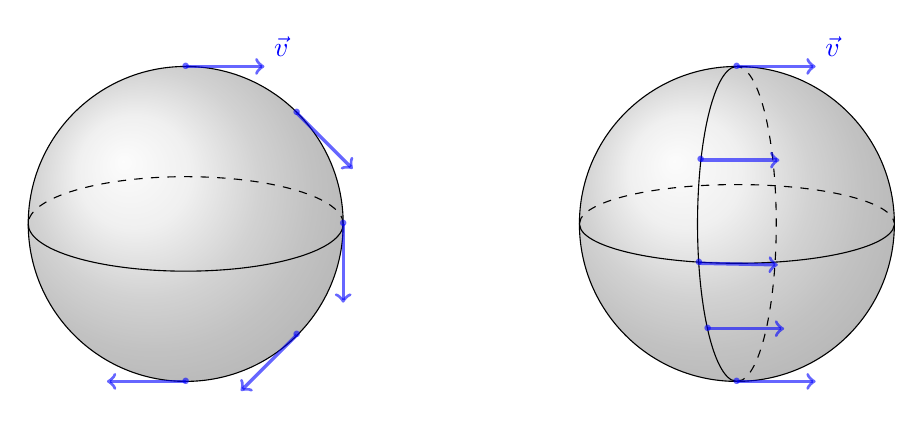
\begin{tikzpicture}[scale = 1]
                            \shade[ball color = gray!40, opacity = 0.4] (0,0) circle (2cm);
                            \draw (0,0) circle (2cm);
                            \draw (-2,0) arc (180:360:2 and 0.6);
                            \draw[dashed] (2,0) arc (0:180:2 and 0.6);
                            \draw[->, very thick, blue, opacity = 0.6] (0,2) node[scale = 0.6]{$\bullet$} -- (1, 2);
                            \draw[blue] (1, 2) node[above right]{$\vec{v}$};
                            \draw[->, very thick, blue, opacity = 0.6] (1.41,1.41) node[scale = 0.6]{$\bullet$} -- (2.12, 0.7);
                            \draw[->, very thick, blue, opacity = 0.6] (2,0) node[scale = 0.6]{$\bullet$} -- (2, -1);
                            \draw[->, very thick, blue, opacity = 0.6] (1.41,-1.41) node[scale = 0.6]{$\bullet$} -- (0.7, - 2.12);
                            \draw[->, very thick, blue, opacity = 0.6] (0,-2) node[scale = 0.6]{$\bullet$} -- (-1, -2);
                            
                            \shade[ball color = gray!40, opacity = 0.4] (7,0) circle (2cm);
                            \draw (7,0) circle (2cm);
                            \draw[dashed] plot [domain =-2:2, samples = 200] (\x+7, {(0.5*sqrt(1-((\x)/2)^2)});
                            \draw plot [domain =-2:2, samples = 200] (\x+7, {(-0.5*sqrt(1-((\x)/2)^2)});
                            \draw plot [domain =-2:2, samples = 200] ({(-0.5*sqrt(1-((\x)/2)^2)+7},\x);
                            \draw[dashed] plot [domain =-2:2, samples = 200] ( {(0.5*sqrt(1-((\x)/2)^2)+7},\x);
                            \draw[->, very thick, blue, opacity = 0.6] (7,2) node[scale = 0.6]{$\bullet$} -- (8, 2);
                            \draw[blue] (8, 2) node[above right]{$\vec{v}$};
                            \draw[->, very thick, blue, opacity = 0.6] (6.54,0.81) node[scale = 0.6]{$\bullet$} -- (7.54, 0.81);
                            \draw[->, very thick, blue, opacity = 0.6] (6.52,-0.5) node[scale = 0.6]{$\bullet$} -- (7.52, -0.52);
                            \draw[->, very thick, blue, opacity = 0.6] (6.63,-1.33) node[scale = 0.6]{$\bullet$} -- (7.6, -1.33);
                            \draw[->, very thick, blue, opacity = 0.6] (7,-2) node[scale = 0.6]{$\bullet$} -- (8, -2);
                        \end{tikzpicture}
                        \caption{Transport parallèle d'un vecteur tangent à la sphère suivant deux chemins différents}
                    \end{figure}
                \end{exmp}
                
                Comment faire pour que le transport parallèle ne dépende pas du chemin en question? Prenons des chemins infinitésimaux.
                %schéma eliott
                
                Le transport parallèle du vecteur $V$ en $P$ le long du chemin infinitésimale donne un vecteur $\widetilde{V}$ en $P$. Pour cela, on doit faire une intégration infinitésimale de l'équation \ref{eq:transportv}.
                
                \begin{prop}\begin{leftbar}
                    La solution de l'équation
                    \begin{equation}
                        \frac{dV^a}{d\lambda} + \Gamma^a_{\mu b}\frac{dx^\mu}{d\lambda} = 0
                    \end{equation}
                    est 
                    \begin{equation}
                        V(\lambda) = \left[P(0)e^{-\int_0^\lambda d\widetilde{\lambda}V(\widetilde{\lambda})}\right]V(0)
                    \end{equation}
                    où les \textit{produit ordonné} $P$ est défini comme
                    \begin{equation}
                        P\left(V(\lambda_1)V(\lambda_2)\right) ~\hat{=}~ V(\lambda_1) V(\lambda_2)\theta(\lambda_1-\lambda_2)+V(\lambda_2) V(\lambda_1)\theta(\lambda_2-\lambda_1).
                    \end{equation}
                \end{leftbar}\end{prop}
                
                \begin{proof}
                    Cette équation peut être réécrite comme
                    \begin{equation}
                        \frac{dV}{d\lambda} = -A(\lambda)V
                    \end{equation}
                    avec $A(\lambda) = \Gamma_\mu \frac{dx^\mu}{d\lambda}$. La forme intégrale de cette équation est 
                    \begin{equation}
                        V(\lambda) = V(0) - \int_0^\lambda d\lambda_1 A(\lambda_1)V(\lambda_1)
                    \end{equation}
                    C'est une équation équivalente. On peut trouver une solution formelle à cette équation en utilisant une méthode perturbative. En substituant cette équation dans elle-même, nous obtenons
                    \begin{equation}
                        V(\lambda) = V(0) - \int_0^\lambda d\lambda_1 A(\lambda_1)V(0)+\int_0^\lambda d\lambda_1\int_0^{\lambda_1}d\lambda_2A(\lambda_1)A(\lambda_2)V(\lambda_2).
                    \end{equation}
                    
                    On peut répéter ce processus une infinité de fois pour trouver
                    \begin{equation}
                        V(\lambda) = V(0) + \sum_{n=1}^\infty\frac{(-1)^n}{n!}\int_{0\leq\lambda_n\leq\lambda_{n-1}}d\lambda_1\dots d\lambda_n A(\lambda_1)\dots A(\lambda_n)V(\lambda_n).
                    \end{equation}
        
                    Les variables d'intégration $\lambda_1,\dots,\lambda_n$ satisfont $\lambda\geq\lambda_1\geq\dots\geq\lambda_n\geq0$ ce qui permet dé réécrire cette équation avec une seule intégral et des fonction $\theta$ de de Heaviside.
                    
                    \begin{align}
                        V(\lambda) &= V(0) + \sum_{n=1}^\infty\frac{(-1)^n}{n!}\int_{0\leq\lambda_n\leq\lambda_{n-1}}d\lambda_1\dots d\lambda_n V(\lambda_1)\dots V(\lambda_n)\theta(\lambda_1-\lambda_2)\dots\theta(\lambda_{n-1}-\lambda_n) \\
                        &= V(0) + \sum_{n=1}^\infty\frac{(-1)^n}{n!}\int_{0\leq\lambda_n\leq\lambda_{n-1}}d\lambda_1\dots d\lambda_n P\left(V(\lambda_1)\dots V(\lambda_n)\right)\\
                        &= \left[P(0)e^{-\int_0^\lambda d\widetilde{\lambda}V(\widetilde{\lambda})}\right]V(0)
                    \end{align}
                \end{proof}
                
                \begin{rmk}
                    La méthode perturbative utilise dans le démonstration précédente est très utilisée en QFT. Dans ce cas, on utilise le produit chronologique $T$ (pour "time ordered") au lieu de produit ordonnée $P$ (pour "path ordered") car les variables d'intégration sont les variables temporelles.
                \end{rmk}
                
                Dans notre cas, comme il s'agit de chemins infinitésimaux, on peut se limiter à un développement à l'ordre quadratique. On peut montré que développer au premier ordre n'est pas suffisant.
                \begin{equation}
                        V(\lambda_2) = V(0) - \int_1^\lambda d\lambda_2 A(\lambda')V(\lambda_1)+\frac{1}{2}\int_{\lambda_1}^{\lambda_2} d\lambda'\int_{\lambda_1}^{\lambda'}d\lambda''A(\lambda')A(\lambda')V(\lambda_1).
                    \end{equation}
                Notons $V(\lambda_1)\equiv V_1$ et $V(\lambda_2)\equiv V_2$. Dans ce cas, en utilisant la forme explicite de $A$, on trouve que 
                \begin{equation}
                    V_2^\mu = V_1^\mu - \oint \Gamma^\mu_{\nu\rho} dx^\nu V_1^\rho+\frac{1}{2}\int_{\lambda_1}^{\lambda_2} d\lambda'\int_{\lambda_1}^{\lambda'}d\lambda''A^\mu_{~\sigma}(\lambda')A^\sigma_{~\kappa}(\lambda'')V_1^\kappa.
                \end{equation}
                En notation matricielle, 
                \begin{equation}
                    V_2 = V_1 - \oint \Gamma V_1+\frac{1}{2}\int_{\lambda_1}^{\lambda_2} d\lambda'\int_{\lambda_1}^{\lambda'}d\lambda''\Gamma_\rho(\lambda_1)\Gamma_\xi(\lambda'')\frac{dx^\rho}{d\lambda'}\frac{dx^\xi}{d\lambda''} V_1.
                \end{equation}
                Par le théorème de Stokes,
                \begin{equation}
                     \oint \Gamma V_1 = \int_\Sigma d\gamma V_1
                \end{equation}
                avec $\Sigma$ telle que $\p\mathscr{C}$. Le terme $\Gamma_\rho(\lambda_1)\Gamma_\xi(\lambda'')$ peut s'exprimer comme $\eval{\Gamma_\rho\Gamma_\xi}_\mathscr{C}$ plus des corrections qui diminuent avec la taille du contour. On peut donc les négliger.
                \begin{equation}
                    V_2 = V_1-\int_\Sigma v_1 d\Gamma + \Gamma_\rho\Gamma_\xi \int_{\lambda_1}^{\lambda_2}d\lambda'\frac{dx^\rho}{d\lambda'}(\x^\xi(\lambda')-x^\xi(\lambda_1))V_1+\dots
                \end{equation}
                Or, si l'on intègre par partie,
                \begin{equation}
                    \int x^\xi dx^\rho = -\oint x^\rho dx^\xi = \int_\Sigma dx^\xi\wedge dx^\rho = \int_\Sigma d(x^\xi dx^\rho) = \text{aire de }\Sigma
                \end{equation}
                car le chemin est fermé. Finalement, on peut écrire $V_2$ comme
                \begin{align}
                    V_2 &= V_1-\int_\Sigma V_1 d\Gamma + \Gamma_\rho\Gamma_\xi\oint V_1x^\xi dx^\rho +\dots\\
                    &= \left( \mathbb{1}-\int_\Sigma d\Gamma + \Gamma_\rho\Gamma_\xi \int dx^\xi\wedge dx^\rho+\dots \right)V_1 \\
                    &= \left( \mathbb{1}-\int_\Sigma d\Gamma+\Gamma\wedge\Gamma \right)V_1 \\
                    &= \left( \mathbb{1}-\int_\Sigma \mathscr{R} \right)V_1
                \end{align}
                On a obtenu une formule complètement géométrique qui fait apparaître $\mathscr{R}$. On voit que le courbure est le générateur infinitésimale du transport parallèle le long d'un contour fermé.\\
                
                Le résultat s'écrit de manière très élégante :
                \begin{equation}
                    \widetilde{V}^a(P) = \int_\Sigma \mathscr{R}^a_{~b} V^b(P)
                \end{equation}
                où $\Sigma = \p\mathscr{C}$. C'est une version généralisée du théorème de Stokes.\\
                
                Par conséquent, si $\mathscr{R} = 0$, $V_2 = V_1$ le long d'un transport parallèle le long d'un contour fermé. Ceci implique que $V_2 = V_1$ le long d'un contour fermé de taille finie. En effet, on peut toujours décomposé un contour fermé de taille finie en une somme de contours fermé de taille infinitésimale.\\
                
                Ceci montre que si $\mathscr{R} = 0$ et $\{e_a(P)\}$ est une base de $\F_P$, alors on peut définir une base $\{e_a(Q)\}$ pour tout $Q\in\M$ en transportant parallèlement les vecteur de $\{e_a(P)\}$ en $Q$ le long d'un contour joignant $P$ à $Q$. Dans une telle base, $\nabla_{e_a} = 0$ et donc $\Gamma = 0$.\\
                
                Dans le cadre de la relativité générale, ceci implique que si $R_{\mu\nu\rho\sigma} = 0$, alors il existe un référentiel dans lequel $g = \eta$ partout : on a affaire à un espace plat.\\
            
                Nous allons maintenant nous intéresser à deux identité très importants : les identités de Bianchi.
                
                \begin{prop}[première identité de Bianchi]\begin{leftbar}
                    Soit $T$ le tenseur de torsion et $\{e_a\}$ une base de $T_P\M$. Dans ce cas,
                    \begin{equation}
                        dT = \mathscr{R} \wedge e - \Gamma\wedge T
                    \end{equation}
                \end{leftbar}\end{prop}
                
                \begin{proof}
                    Il suffit de partir de la définition $T = de+\Gamma\wedge e$.
                    \begin{align}
                        dT &= d\Gamma\wedge e - \Gamma \wedge de\\
                        &= (\mathscr{R}-\Gamma\wedge\Gamma)\wedge e-\Gamma\wedge(T-\Gamma\wedge e)\\
                        &= \mathscr{R} \wedge e - \Gamma\wedge T
                    \end{align}
                \end{proof}
                
                \begin{prop}[deuxième identité de Bianchi]\begin{leftbar}
                    Soit $T$ le tenseur de torsion et $\{e_a\}$ une base de $T_P\M$. Dans ce cas,
                    \begin{equation}
                        d\mathscr{R} = \mathscr{R} \wedge \Gamma - \Gamma\wedge \mathscr{R}
                    \end{equation}
                \end{leftbar}\end{prop}
                
                \begin{proof}
                    Il suffit de partir de la définition $\mathscr{R} = d\Gamma+\Gamma\wedge\Gamma$.
                    \begin{align}
                        d\mathscr{R} &= d\Gamma\wedge\Gamma-\Gamma\wedge d\Gamma\\
                        &= (\mathscr{R}-\Gamma\wedge\Gamma)\wedge\Gamma - \Gamma\wedge(\mathscr{R}-\Gamma\wedge\Gamma)\\
                        &= \mathscr{R} \wedge \Gamma - \Gamma\wedge \mathscr{R}
                    \end{align}
                \end{proof}
                
                Dans le cas où $T = 0$, la première identité de Bianchi donne
                \begin{align}
                    0 &= \mathscr{R}\wedge e\\
                    &= \mathscr{R}^a_{~d}\wedge e^d\\
                    &= \mathscr{R}^a_{~dbc}\wedge e^b\wedge e^c\wedge e^d \\
                    &= \mathscr{R}^a_{~[bcd]}\\
                    &= \mathscr{R}^a_{~bcd}+\mathscr{R}^a_{~dbc}+\mathscr{R}^a_{~cdb}\label{eq:idbianchi}
                \end{align}
                
            \subsection{Cas de la connexion de Levi-Civita}
                        
                Dans cette section nous allons particulariser les résultats généraux qui ont été étudiés au cas de la relativité générale. On prend la métrique $g$ et la connexion de Levi-Civita. \\
                
                Dans ce cas-ci, les indices de fibre $a$ et $b$ et les indices d'espace tangent $\mu$ et $\nu$ sont de même nature. Ceci implique que $\mathscr{R}^a_{~b\mu\nu}$ est un tenseur.
                \begin{equation*}
                    \mathscr{R}^\rho_{~\sigma\mu\nu}\to R^\rho_{~\sigma\mu\nu}
                \end{equation*}
                
                \begin{definition}
                    Le tenseur de composantes 
                    \begin{equation}
                        R^\rho_{~\sigma\mu\nu} = \p_\rho\Gamma^\mu_{\sigma \nu}-\p_\sigma\Gamma^\mu_{\rho\nu} + \Gamma^\mu_{\rho \theta}\Gamma^\theta_{\sigma\nu}-\Gamma^\mu_{\sigma \theta}\Gamma^\theta_{\rho\nu}
                    \end{equation}
                    est de type $(3,1)$ est appelé $\textit{tenseur de Riemann}$.
                \end{definition}
                
                \begin{prop}\begin{leftbar}
                    Le tenseur de Riemann a les propriétés suivantes:
                    \begin{enumerate}[label = \textit{\roman*)}]
                        \item anti-symétrie par rapport aux deux premiers indices :
                        \begin{equation}
                            R_{\mu\nu\sigma\rho} = -R_{\nu\mu\sigma\rho}
                        \end{equation}
                        \item symétrie par rapport aux couples d'indices successifs :
                        \begin{equation}
                            R_{\mu\nu\sigma\rho} = R_{\sigma\rho\mu\nu}
                        \end{equation}
                        \item anti-symétrie par rapport aux deux derniers indices :
                        \begin{equation}
                            R_{\mu\nu\sigma\rho} = -R_{\nu\mu\sigma\rho}
                        \end{equation}
                        \item \textit{première identité de Bianchi} :
                        \begin{equation}
                        R_{\mu\nu\sigma\rho}+R_{\mu\rho\nu\sigma}+R_{\mu\sigma\rho\nu} = 0
                        \end{equation}
                        Nous faisons une permutation cyclique des trois dernier indices.
                        \item \textit{deuxième identité de Bianchi} :
                        \begin{equation}
                            \nabla_\mu R_{\nu\rho\sigma\theta} + \nabla_\theta R_{\nu\rho\mu\sigma}+\nabla_\sigma R_{\nu\rho\theta\mu} = 0
                        \end{equation}
                        Nous faisons une permutation cyclique de l'indice de $\nabla$ et des deux dernier indices de $R$.
                    \end{enumerate}
                \end{leftbar}\end{prop}
                
                \begin{proof}${}$\\
                    \begin{enumerate}[label = \textit{\roman*)}]
                        \item Voir début du cours.
                        \item Voir début du cours. Notons que ce résultat n'est vrai que pour la connexion de Levi-Civita.
                        \item Direct d'après les deux premières propriétés.
                        \item Nous avons montré que la connexion de Levi-Civita est de torsion nulle. Ceci implique que la formule \ref{eq:idbianchi} est valable.
                        \item On sait que, pour $T\in\M$, il existe une base localement plate $(x^\alpha_P)$ dans laquelle $\Gamma = 0$ (montré dans la section précédente). Dans cette base, la deuxième identité de Bianchi prend la forme
                        \begin{equation}
                            dR = 0
                        \end{equation}
                        ou encore
                        \begin{align}
                            0 &= dR^\alpha_{~\beta} = \frac{1}{2} \p_\varepsilon R^\alpha_{~\beta\gamma\delta}~dx^\varepsilon\wedge dx^\gamma\wedge dx^\delta \\
                            \Leftrightarrow\qquad 0 &= \p_\varepsilon R^\alpha_{~\beta\gamma\delta} + \p_\gamma R^\alpha_{~\beta\delta\epsilon} + \p_\delta R^\alpha_{~\beta\gamma\varepsilon}
                        \end{align}
                        Il suffit juste d'utiliser le fait que $\nabla_\mu = \p_\mu$ dans des coordonnées locales plates et on trouve bien la relation voulue. Nous avons montré que le résultat étant vrai dans un système de coordonnée en particulier. Comme $R$ est un tenseur, cela reste vrai dans tout les autre système de coordonnées.
                    \end{enumerate}
                \end{proof}
                
                \begin{prop}\begin{leftbar}
                    Le nombre de composantes indépendantes du tenseur de Riemann est
                    \begin{equation}
                        \frac{1}{12}D^2(D^2-1).
                    \end{equation}
                    En particulier pour $n=4$, les tenseur de Riemann possède $20$ composantes indépendantes.
                \end{leftbar}\end{prop}
                
                \begin{proof}
                    Le nombre de composantes indépendantes d'un tenseur de rang $4$ qui ets symétrique sous l'échange des couples d'indices successifs est 
                    \begin{equation}
                        \frac{1}{2}D(D-1)\frac{1}{2}D(D-1)
                    \end{equation}
                    Si de plus ce tenseurs est anti-symétrique sous l'échange des premiers indices, alors ce nombre de devient
                    \begin{equation}
                        \frac{1}{2}\frac{1}{2}D(D-1)\left( \frac{1}{2}D(D-1)1+ \right).
                    \end{equation}
                    Pour tenir compte de l'identité de Bianchi, on observe que le tenseur
                    \begin{equation}
                        t_{\mu\nu\sigma\rho} = R_{\mu\nu\sigma\rho}+R_{\mu\rho\nu\sigma}+R_{\mu\sigma\rho\nu}
                    \end{equation}
                    est complètement anti-symétrique. Le nombre de composantes indépendantes final est donc 
                    \begin{equation}
                        \frac{1}{2}\frac{1}{2}D(D-1)\left( \frac{1}{2}D(D-1)1+ \right)  -\frac{D(D-1)(D-2)(D-3)}{4!}.
                    \end{equation}
                \end{proof}
                
                Pour rappel, le nombre d'invariantes de courbure est le nombre de quantités scalaires indépendantes que l'on peut construire avec $R$ et $g$.